\documentclass[a4paper, 11pt]{article}

%%% Работа с русским языком
\usepackage{cmap}					% поиск в PDF
\usepackage{mathtext} 				% русские буквы в формулах
\usepackage[T2A]{fontenc}			% кодировка		% кодировка исходного текста
\usepackage[english,russian]{babel}	% локализация и переносы

%%% Дополнительная работа с математикой
\usepackage{amsfonts,amssymb,amsthm,mathtools} % AMS
\usepackage{amsmath}
\usepackage{icomma} % "Умная" запятая: $0,2$ --- число, $0, 2$ --- перечисление

\usepackage{indentfirst} % Красная строка в начале абзацев

\usepackage{setspace} % Междустрочный интервал
\singlespacing

\usepackage[left=20mm, top=10mm, right=10mm, bottom=25mm, nohead, footskip=7mm]{geometry} % поля документа

%% Номера формул
%\mathtoolsset{showonlyrefs=true} % Показывать номера только у тех формул, на которые есть \eqref{} в тексте.

%% Шрифты
\usepackage{euscript}	 % Шрифт Евклид
\usepackage{mathrsfs} % Красивый матшрифт

%% Перенос знаков в формулах (по Львовскому)
\newcommand*{\hm}[1]{#1\nobreak\discretionary{}
    {\hbox{$\mathsurround=0pt #1$}}{}}

%%% Работа с картинками
\usepackage{graphicx}  % Для вставки рисунков
\graphicspath{{images/}{images2/}}  % папки с картинками
\setlength\fboxsep{3pt} % Отступ рамки \fbox{} от рисунка
\setlength\fboxrule{1pt} % Толщина линий рамки \fbox{}
\usepackage{wrapfig} % Обтекание рисунков и таблиц текстом

%%% Работа с таблицами
\usepackage{array,tabularx,tabulary,booktabs} % Дополнительная работа с таблицами
\usepackage{longtable}  % Длинные таблицы
\usepackage{multirow} % Слияние строк в таблице


\usepackage[utf8]{inputenc}
\usepackage[russian]{babel}
\usepackage{amsmath,amsfonts,amssymb,amsthm,mathtools} %AMS

\usepackage{hyperref}  % Гиперссылки
\usepackage[usernames,dvipsnames,svgnames,table,rgb]{xcolor}
\usepackage{enumitem} %Для нумерации списков
\usepackage{multicol} % Несколько колонок
\usepackage{multirow} % Несколько строк
%\usepackage{caption} % отступы между названием и объектом
%\captionsetup[images]{skip=2ex}

\usepackage{dsfont}

\DeclareMathOperator*{\argmax}{arg\,max}

\hypersetup{
    unicode=true,
    pdftitle={Практическое задание №2}, % Заголовок
    pdfauthor={Кузьмин Никита, ММП 317},
    pdfcreator={Кузьмин Никита, ММП 317},
    colorlinks=false, % false - ссылки в рамках; true - цветные ссылки
    linkcolor=red,   % внутренние ссылки
    citecolor=green, % на библиографию
    filecolor=magenta, % на файлы
    urlcolor=blue % на URL
}



%\usepackage{titlesec}

%\titleformat*{\section}{\LARGE\bfseries}
%\titleformat*{\subsection}{\Large\bfseries}
%\titleformat*{\subsubsection}{\large\bfseries}

\usepackage{sectsty}
\sectionfont{\LARGE}
\subsectionfont{\LARGE}
\subsubsectionfont{\Large}
\usepackage{float}


\usepackage{fancyhdr}% загрузим пакет
%\pagestyle{fancy}% применим колонтитул

\begin{document}
    \hfill Кузьмин Никита, ММП, 317.
    
    \begin{center} \Large Отчет по практическому заданию №2 "\textbf{Применение линейных моделей для определения токсичности комментария}". 
    
    Логистическая регрессия и градиентный спуск.
    \end{center}
    \tableofcontents
    \newpage
    \section{Введение}
    
    В данном документе представлен отчет о проделанных экспериментах по практическому заданию №2, анализ результатов. 
    Краткое описание задания: необходимо реализовать линейный классификатор с произвольной функцией потерь.
    
    \section{Теория}
    
    \section{Эксперименты}
    В этом блоке приведены все обязательные эксперименты, которые изложены в формулировке задания.
    Все эксперименты проводились на упрощенном датасете (рассматривается задача бинарной классификации) из соревнования \textbf{Toxic Comment Classification Challenge}, в котором нужно определить токсичность комментария. 
    
    Стандартный дизайн эксперимента: 
    \begin{itemize}
        \item Оценка качества и подбор параметров модели проводились на каждой эпохе с помощью отложенной тренировочной выборки (30\%). Все графики ниже построены по значениям accuracy, посчитанным на отложенной выборке.
        \item В тренировочную выборку был добавлен признак, состоящий из всех единиц, который позволяет учитывать смещение (\textbf{bias}). Было решено не использовать смещение в $L2$-регуляризации, чтобы даже при плохом выборе коэффициента регуляризации решающая гиперплоскость не вырождалась в 0.
        \item В стохастическом градиентном спуске проверяется критерий останова на каждой эпохе (не итерации).
    \end{itemize}

        \subsection{Исследование поведения градиентного спуска}
            Обновления весов модели при использовании градиетного спуска происходит по следующей формуле:
            \begin{equation}\label{exp1:weight_upd}
            w_t = w_{t-1} - \frac{\alpha}{t^\beta} \times \frac{1}{N} \times \sum_{i=1}^{N}\nabla_{w}\mathcal{L}(x_i, y_i|w_{t-1}),
            \end{equation}
            где $t$ - номер итерации, $\beta$ - \textbf{step\_beta}, $\nabla_{w}\mathcal{L}(x_i, y_i|w_{t-1})$ - градиент функции потерь.
            \subsubsection{Параметр размера шага \textbf{step\_alpha}}
                Параметр \textbf{step\_alpha $(\alpha)$} используется в градиентном спуске при обновлении весов в формуле \ref{exp1:weight_upd}.
                Рассмотрим следующие зависимости при разных значениях параметра \textbf{step\_alpha}:
                    \begin{enumerate}\label{exp:dependencies}
                        \item зависимость значения функции потерь от реального времени работы метода
                        \item зависимость точности (accuracy) от реального времени работы метода
                        \item зависимость значения функции потерь от итерации метода
                        \item зависимость точности (accuracy) от итерации метода
                     \end{enumerate}
                 Соответствующие графики приведены на: рис. \ref{exp1:gd_func_time}, \ref{exp1:gd_acc_time}, \ref{exp1:gd_func_iter}, \ref{exp1:gd_acc_iter}.
   
                 \begin{figure}[H] \label{exp1}
                     \begin{multicols}{2}
                         \begin{center}
                             \caption{Зависимость значения функции потерь от реального времени работы градиентного спуска} \label{exp1:gd_func_time}
                             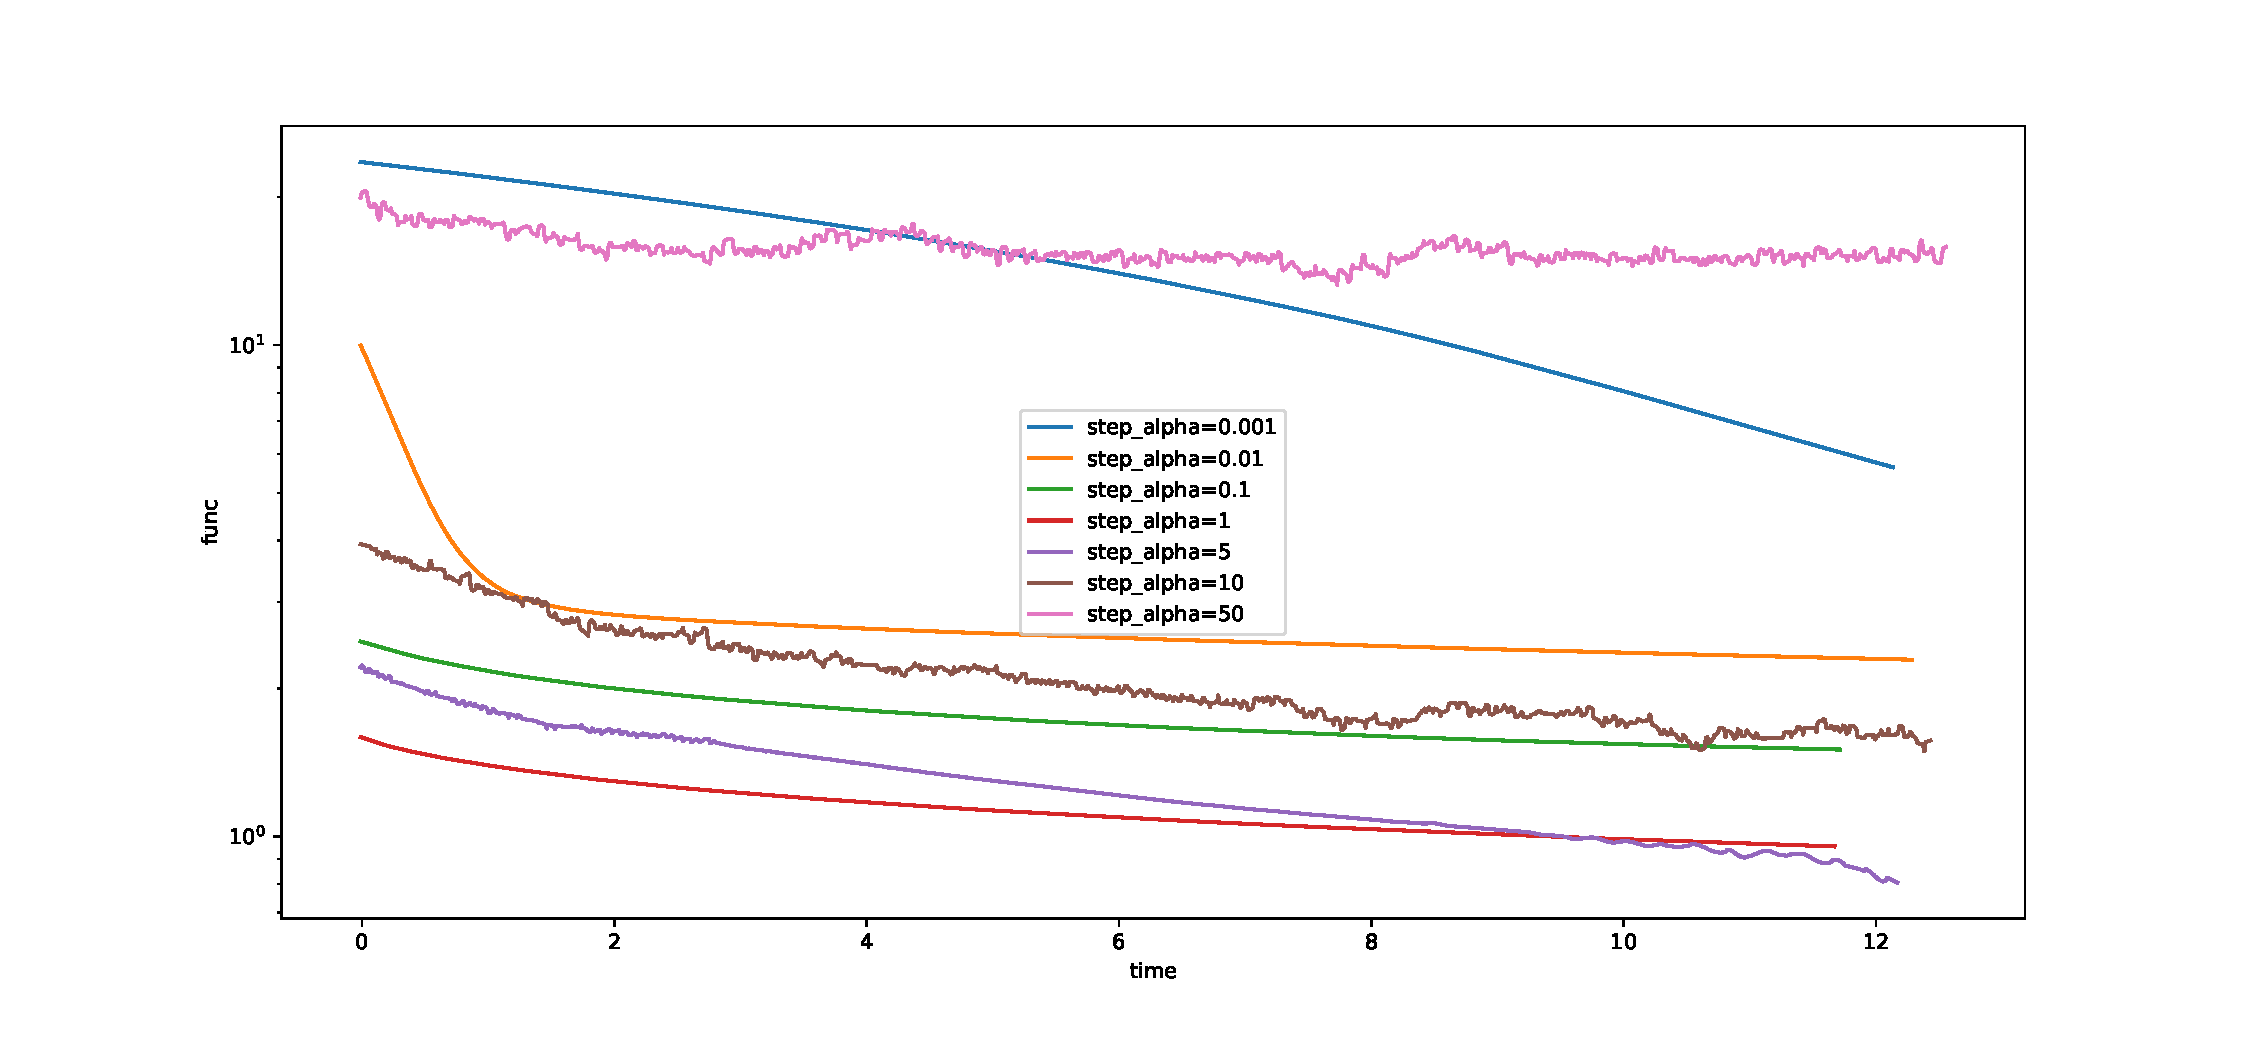
\includegraphics[width=0.5\textwidth, height=0.25\textheight]{../graphs/exp1_func_GD_alpha_time_beta=0,001.pdf}
                             
                             \caption{Зависимость значения точности (accuracy) от реального времени работы градиентного спуска} \label{exp1:gd_acc_time}
                             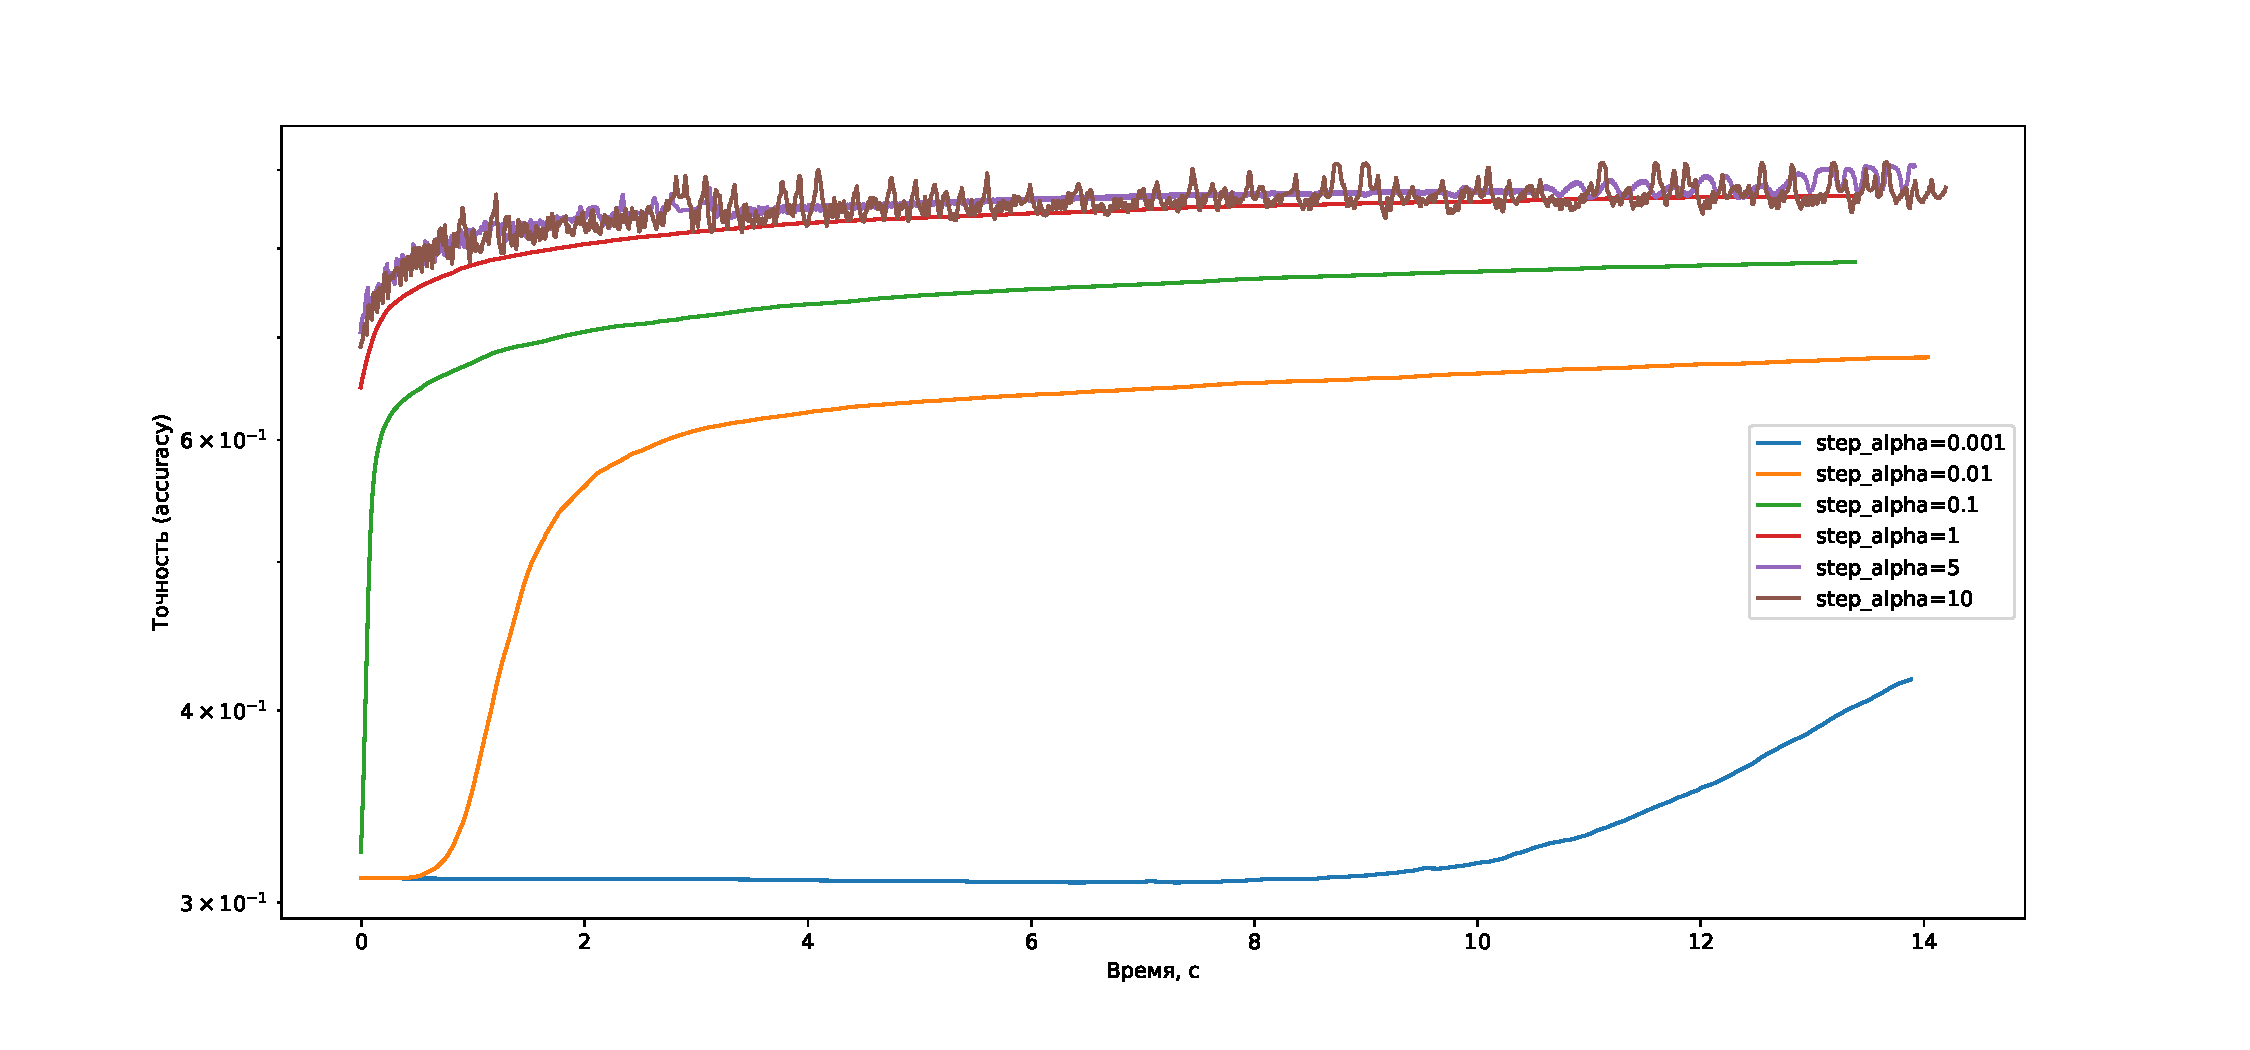
\includegraphics[width=0.5\textwidth, height=0.25\textheight]{../graphs/exp1_accuracy_GD_alpha_time_beta=0,001.pdf}
                             
                             \caption{Зависимость значения функции потерь от итерации метода градиентного спуска} \label{exp1:gd_func_iter}
                             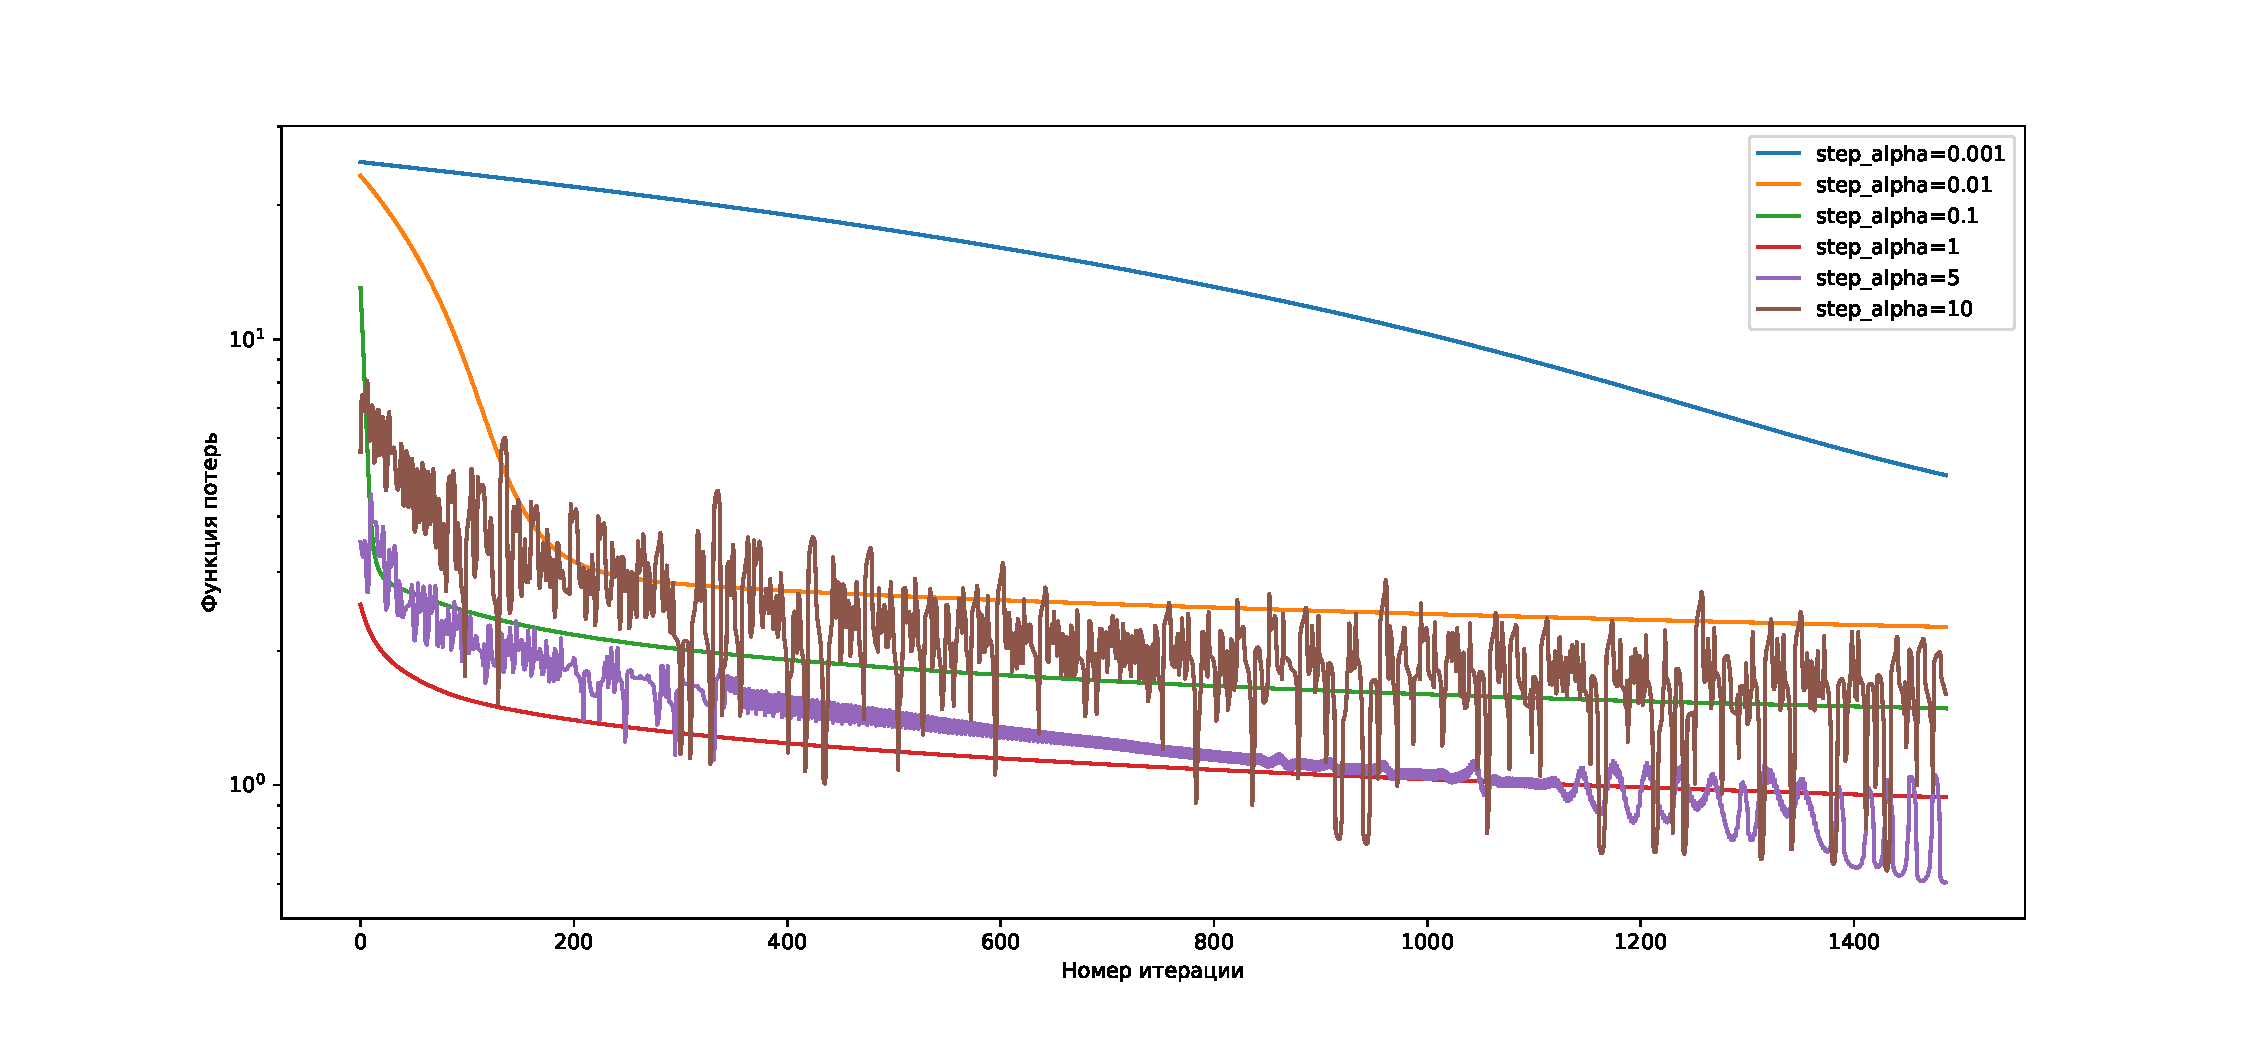
\includegraphics[width=0.5\textwidth, height=0.25\textheight]{../graphs/exp1_func_GD_alpha_iteration_beta=0,001.pdf}
                             
                             \caption{Зависимость значения точности (accuracy) от итерации метода градиентного спуска} \label{exp1:gd_acc_iter}
                             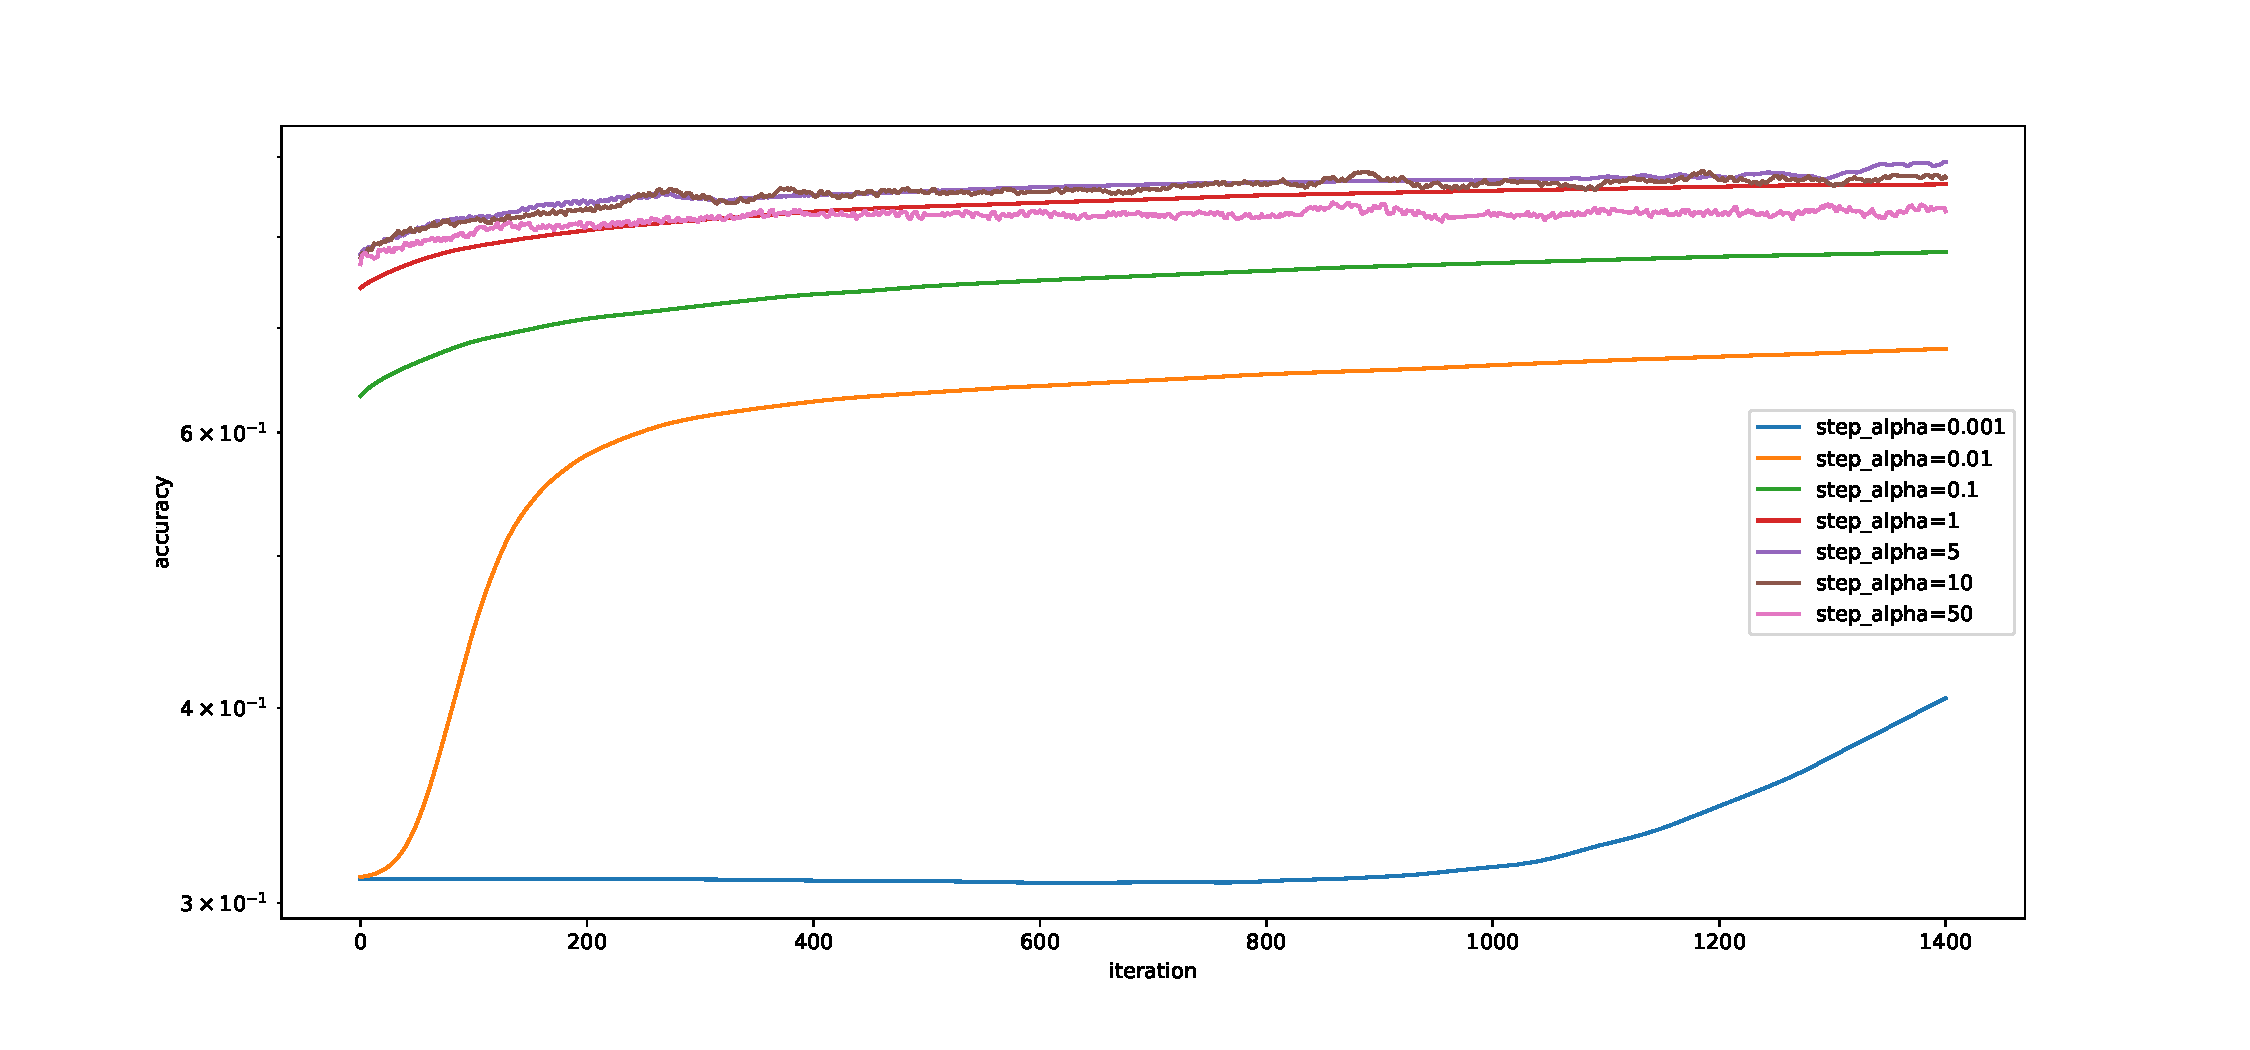
\includegraphics[width=0.5\textwidth, height=0.25\textheight]{../graphs/exp1_accuracy_GD_alpha_iteration_beta=0,001.pdf}
                         \end{center}
                     \end{multicols}
                 \end{figure}
             Из графиков видно, что при значениях $\alpha$, близких к нулю алгоритму нужно больше времени для сходимости. С другой стороны, если значения слишком большие, то алгоритм становится крайне не стабильным.
            \subsubsection{Параметр размера шага step\_beta}
                Параметр \textbf{step\_beta $(\beta)$} используется в градиентном спуске при обновлении весов в формуле \ref{exp1:weight_upd}.
                Аналогично предыдущему пункту рассмотрим зависимости из \ref{exp:dependencies} при разных значениях параметра \textbf{step\_beta} и проанализруем соответсвующие графики, представленные на рис. \ref{exp2:gd_func_time}, \ref{exp2:gd_acc_time}, \ref{exp2:gd_func_iter}, \ref{exp2:gd_acc_iter}.
                
                
                \begin{figure}[H] \label{exp1}
                    \begin{multicols}{2}
                        \begin{center}
                            \caption{Зависимость значения функции потерь от реального времени работы градиентного спуска} \label{exp2:gd_func_time}
                            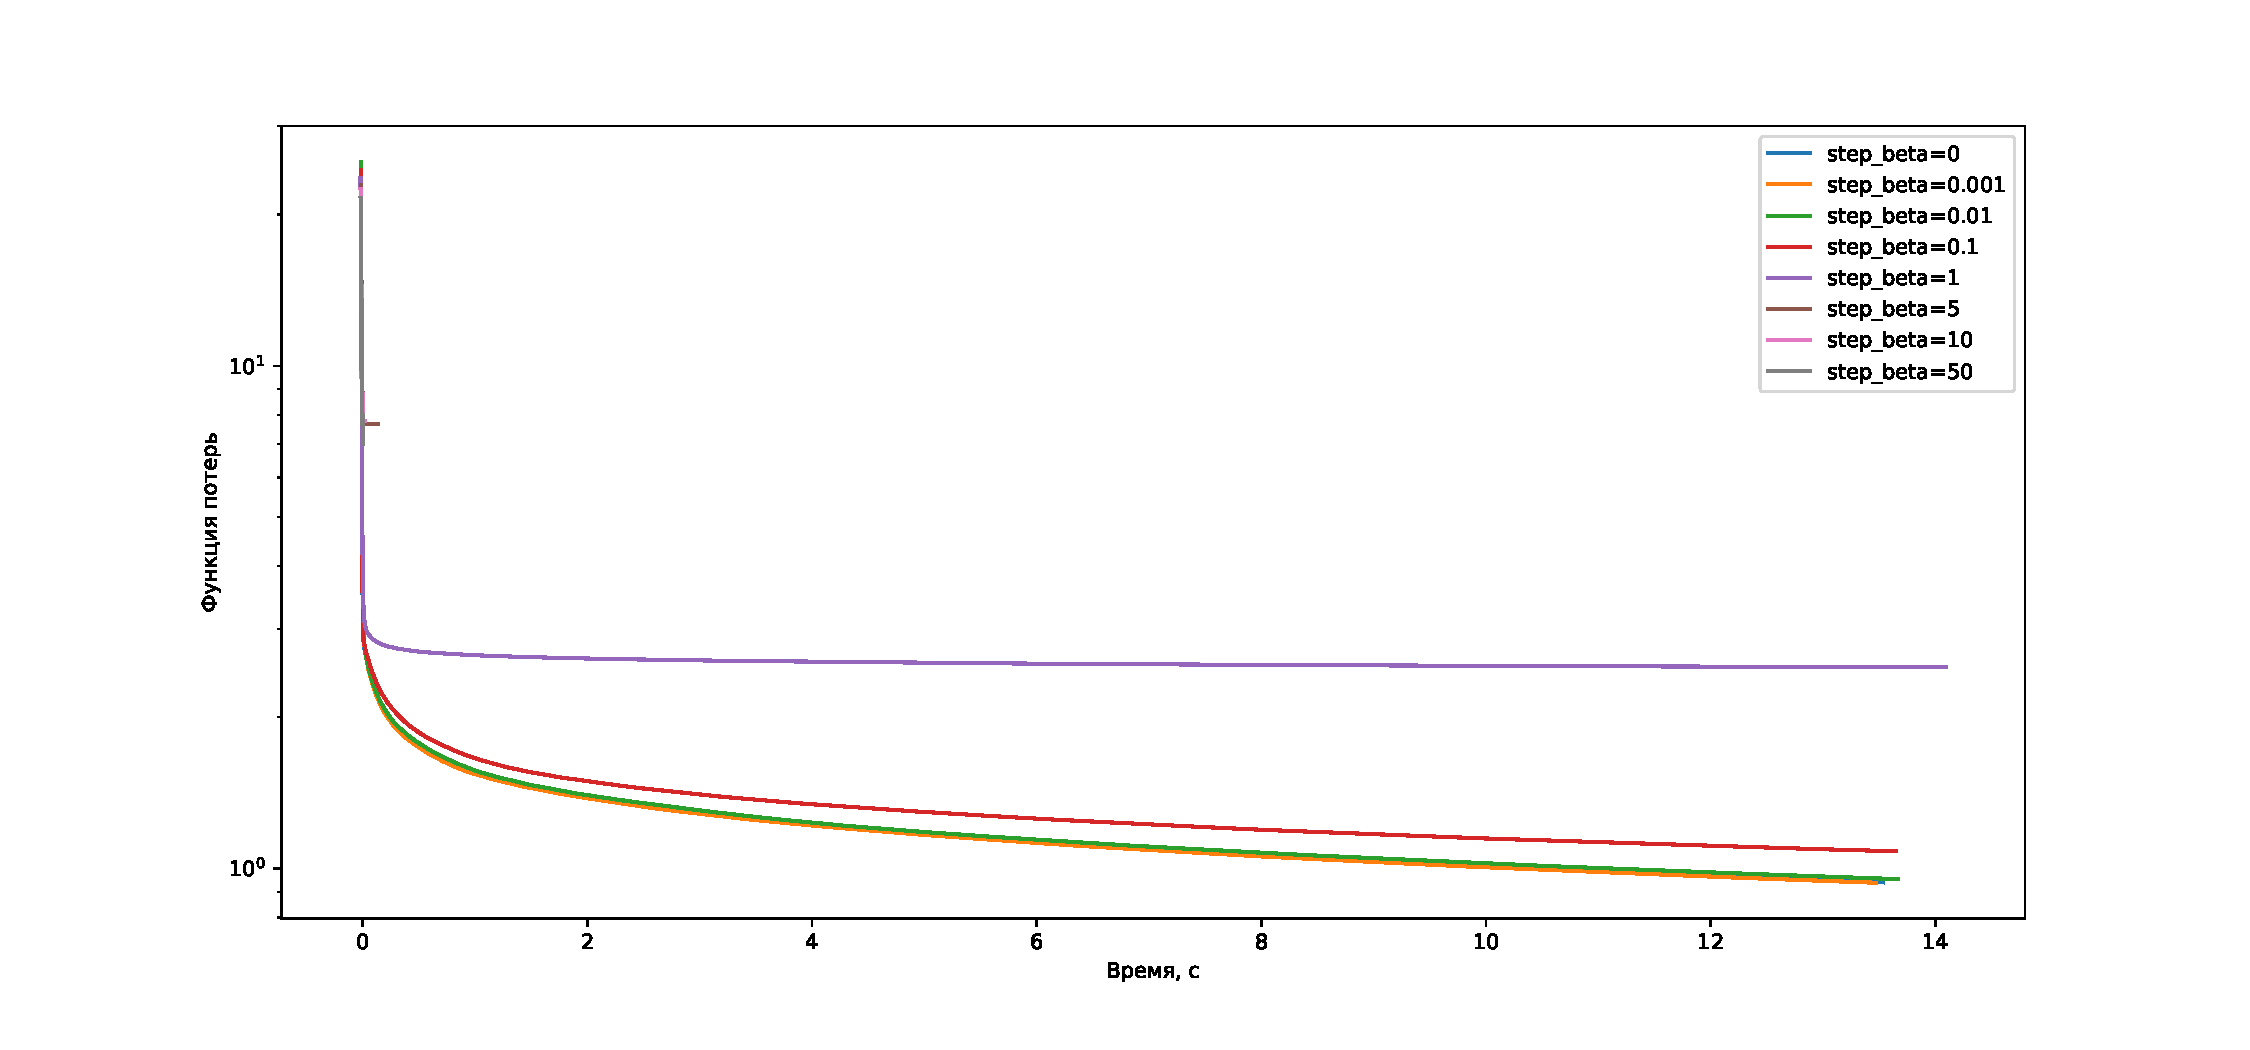
\includegraphics[width=0.5\textwidth, height=0.25\textheight]{../graphs/exp2_func_GD_beta_time_alpha=1.pdf}
                            
                            \caption{Зависимость значения точности (accuracy) от реального времени работы градиентного спуска} \label{exp2:gd_acc_time}
                            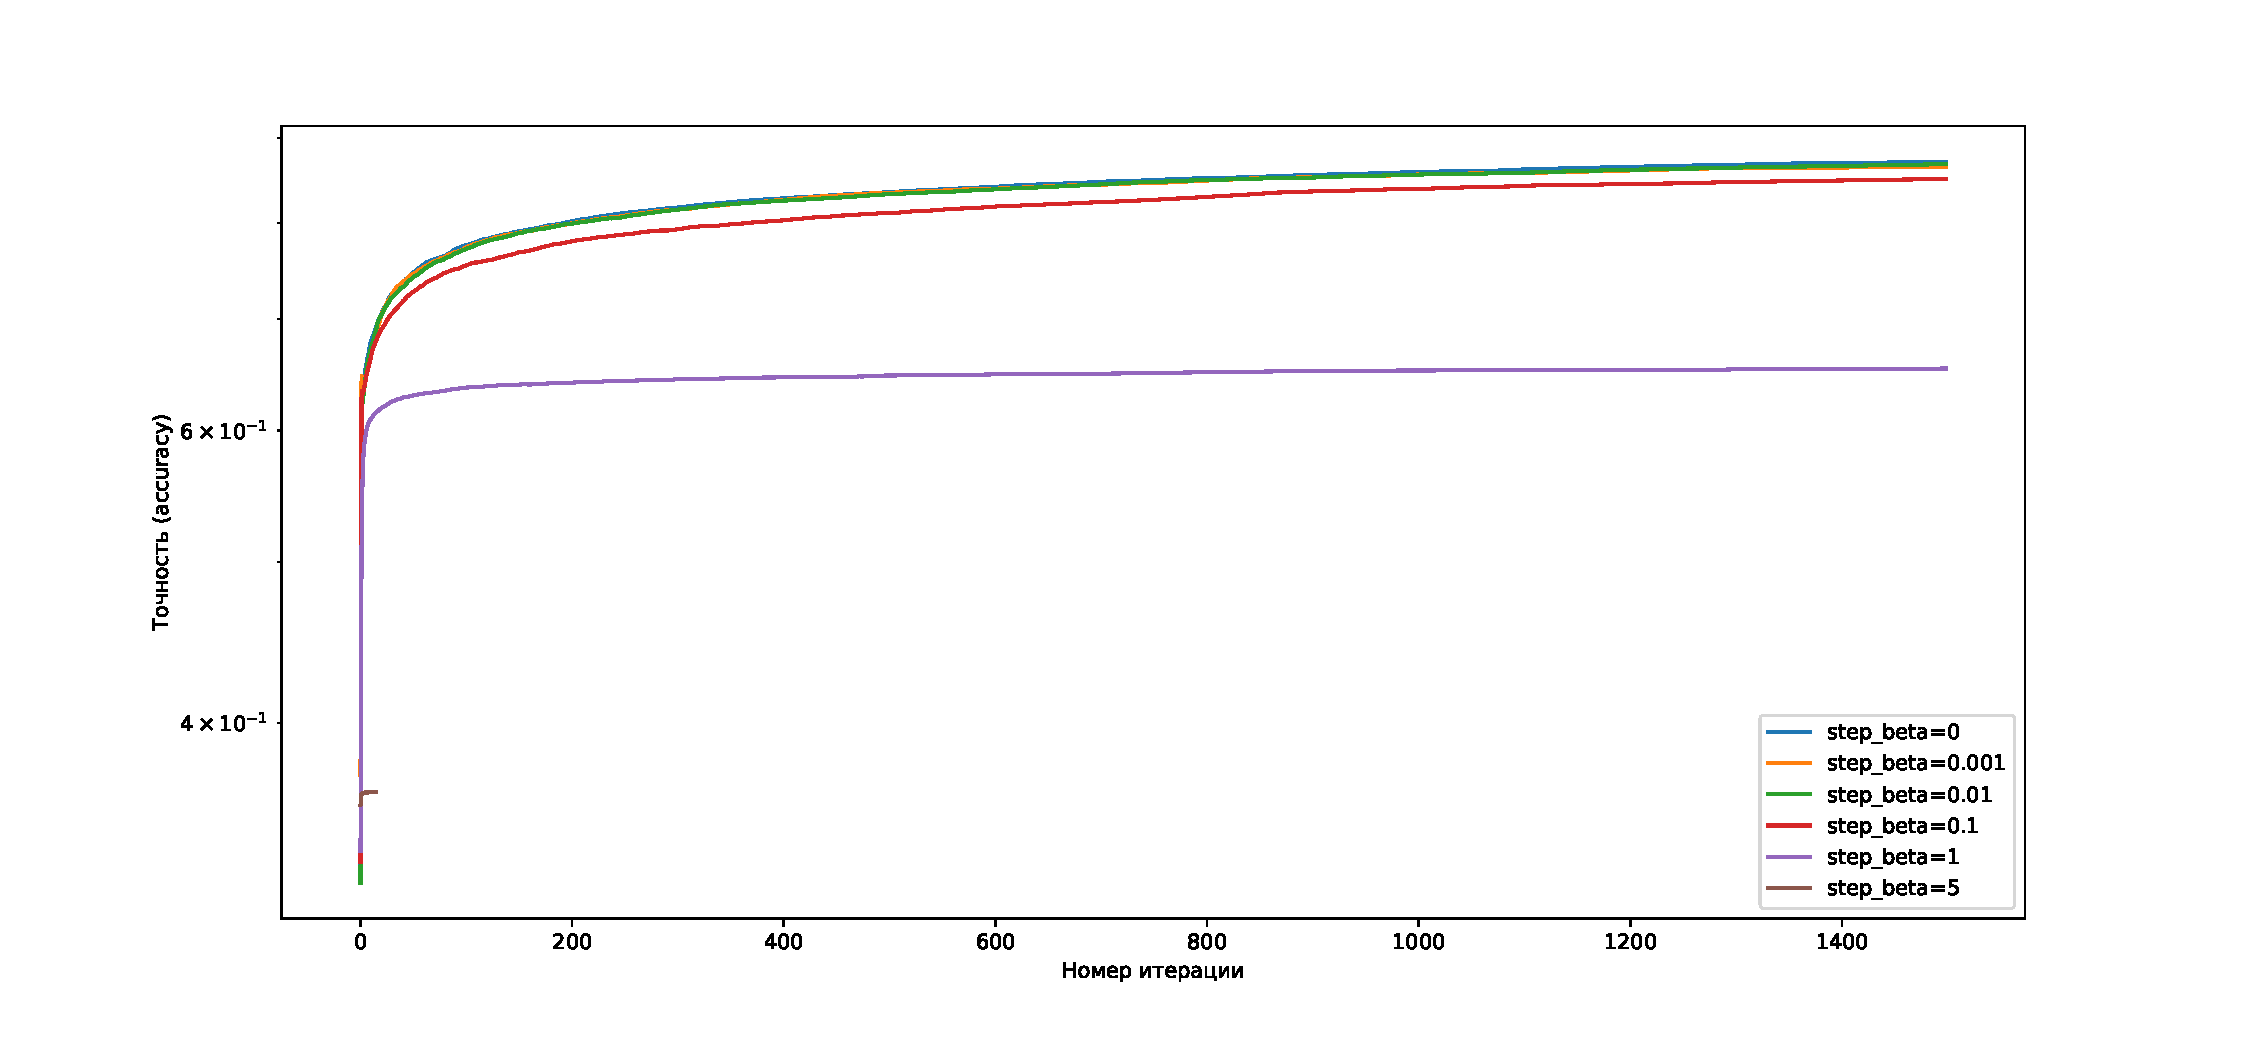
\includegraphics[width=0.5\textwidth, height=0.25\textheight]{../graphs/exp2_accuracy_GD_beta_iteration_alpha=1.pdf}
                            
                            \caption{Зависимость значения функции потерь от итерации метода градиентного спуска} \label{exp2:gd_func_iter}
                            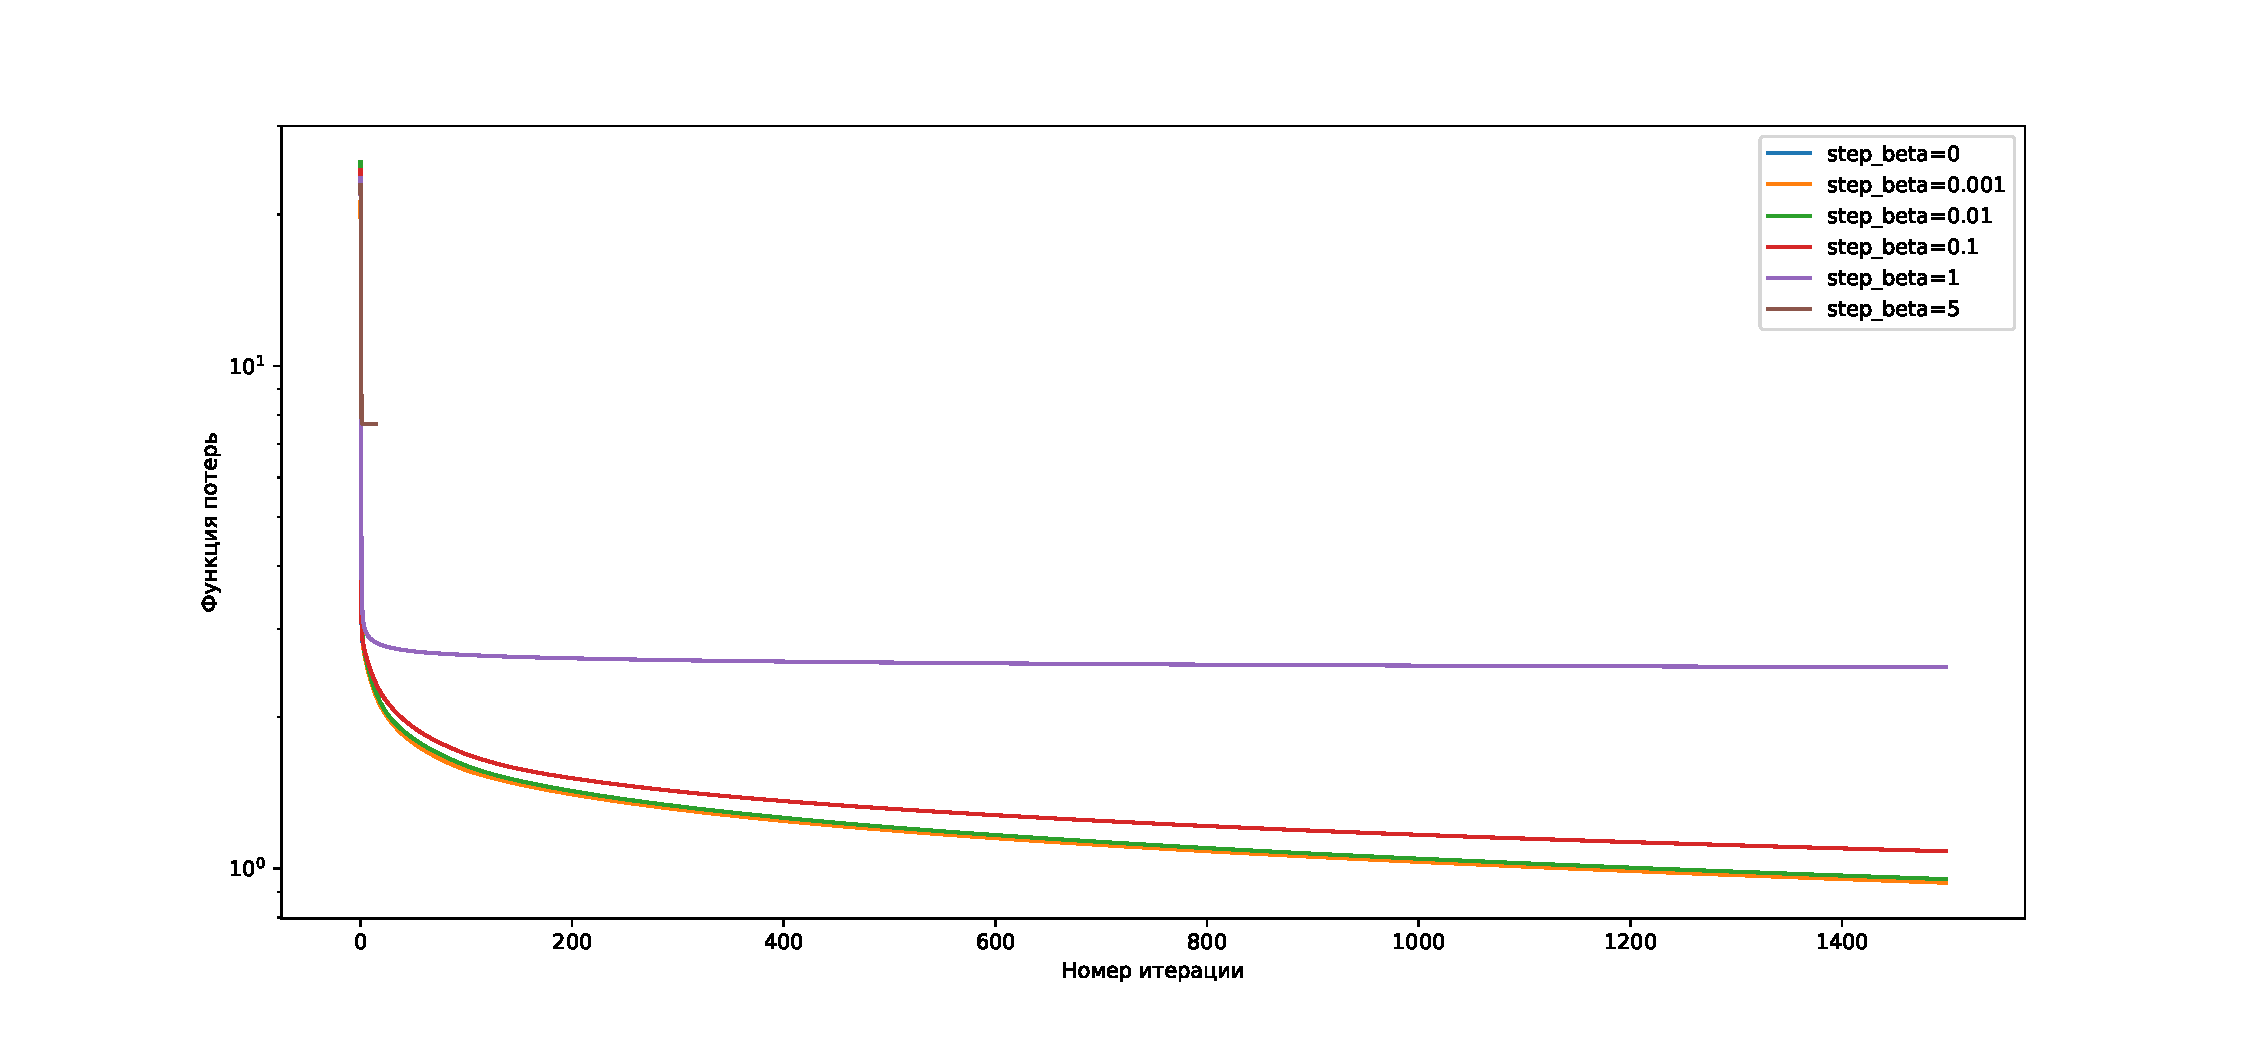
\includegraphics[width=0.5\textwidth, height=0.25\textheight]{../graphs/exp2_func_GD_beta_iteration_alpha=1.pdf}
                            
                            \caption{Зависимость значения точности (accuracy) от итерации метода градиентного спуска} \label{exp2:gd_acc_iter}
                            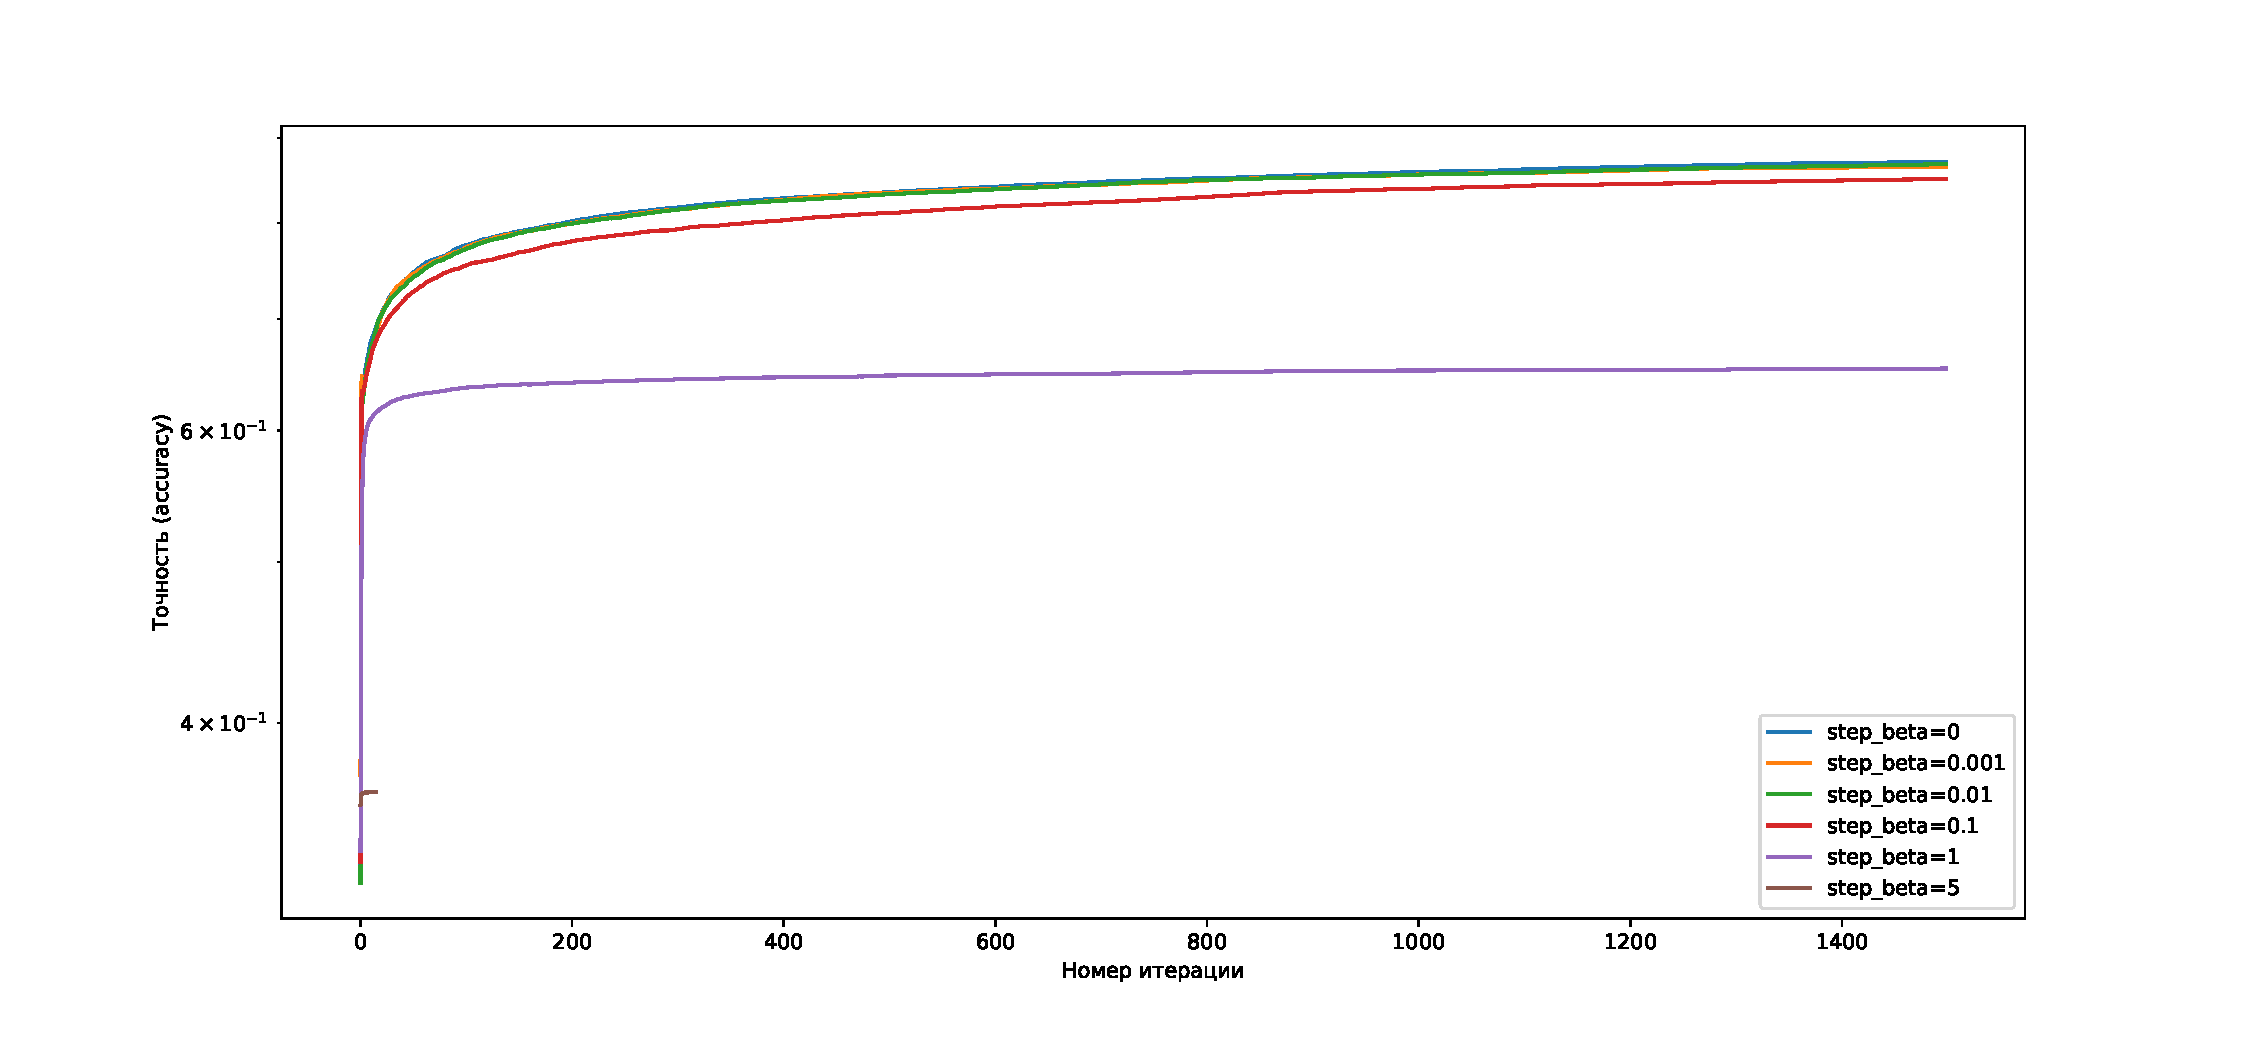
\includegraphics[width=0.5\textwidth, height=0.25\textheight]{../graphs/exp2_accuracy_GD_beta_iteration_alpha=1.pdf}
                        \end{center}
                    \end{multicols}
                \end{figure}
            Из графиков можно заметить, что значения \textbf{step\_beta}, близкие к 0, приводят к одинаковому качеству. С увеличением же параметра \textbf{step\_beta} значение точности уменьшается. При $\textbf{step\_beta = 5}$ изменение функции потерь так мало, что критерий остановки срабатывает до первых 200 итераций.
            
            \subsubsection{Начальное приближение $w_0$}
                Начальное приближение нужно для инициализации весов модели. В данной работе были рассмотрены следующие варианты задания $w_0$:
                \begin{itemize}
                    \item нулевой вектор
                    \item вектор с координатами из $U(0, 1)$
                    \item вектор с координатами из $U(100, 500)$
                    \item вектор с координатами из $U(1000, 5000)$
                    \item вектор с координатами из $U(10000, 50000)$
                    \item вектор с координатами из $N(0, 1)$
                    \item вектор с координатами из $N(0.5, 0.5)$
                \end{itemize}
                Графики зависимостей \ref{exp:dependencies} представлены на рис.  \ref{exp3:gd_func_time}, \ref{exp3:gd_acc_time}, \ref{exp3:gd_func_iter}, \ref{exp3:gd_acc_iter}.
                \begin{figure}[H] \label{exp1}
                    \begin{multicols}{2}
                        \begin{center}
                            \caption{Зависимость значения функции потерь от реального времени работы стохастического градиентного спуска} \label{exp3:gd_func_time}
                            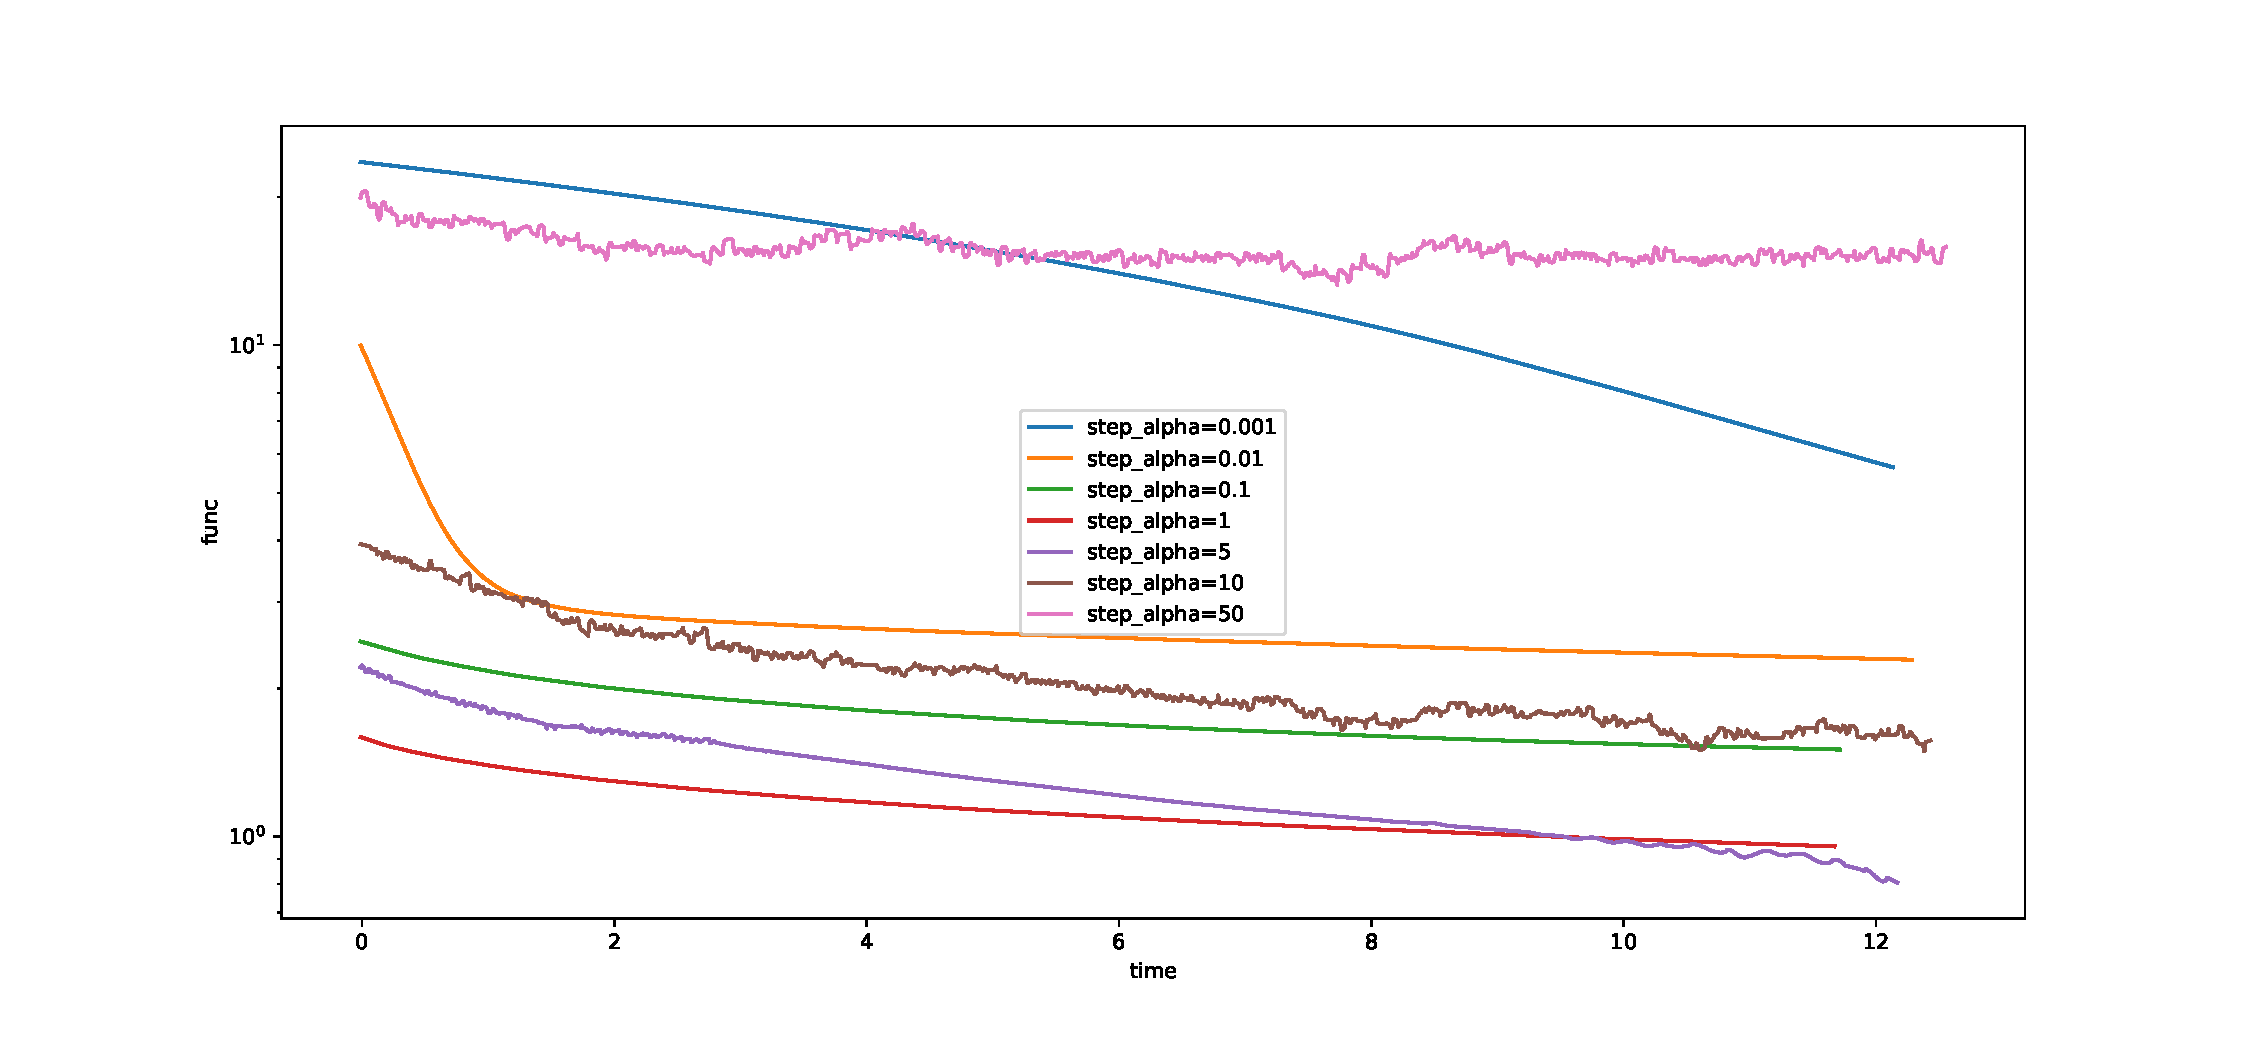
\includegraphics[width=0.5\textwidth, height=0.25\textheight]{../graphs/exp1_func_GD_alpha_time_beta=0,001.pdf}
                            
                            \caption{Зависимость значения точности (accuracy) от реального времени работы стохастического градиентного спуска} \label{exp3:gd_acc_time}
                            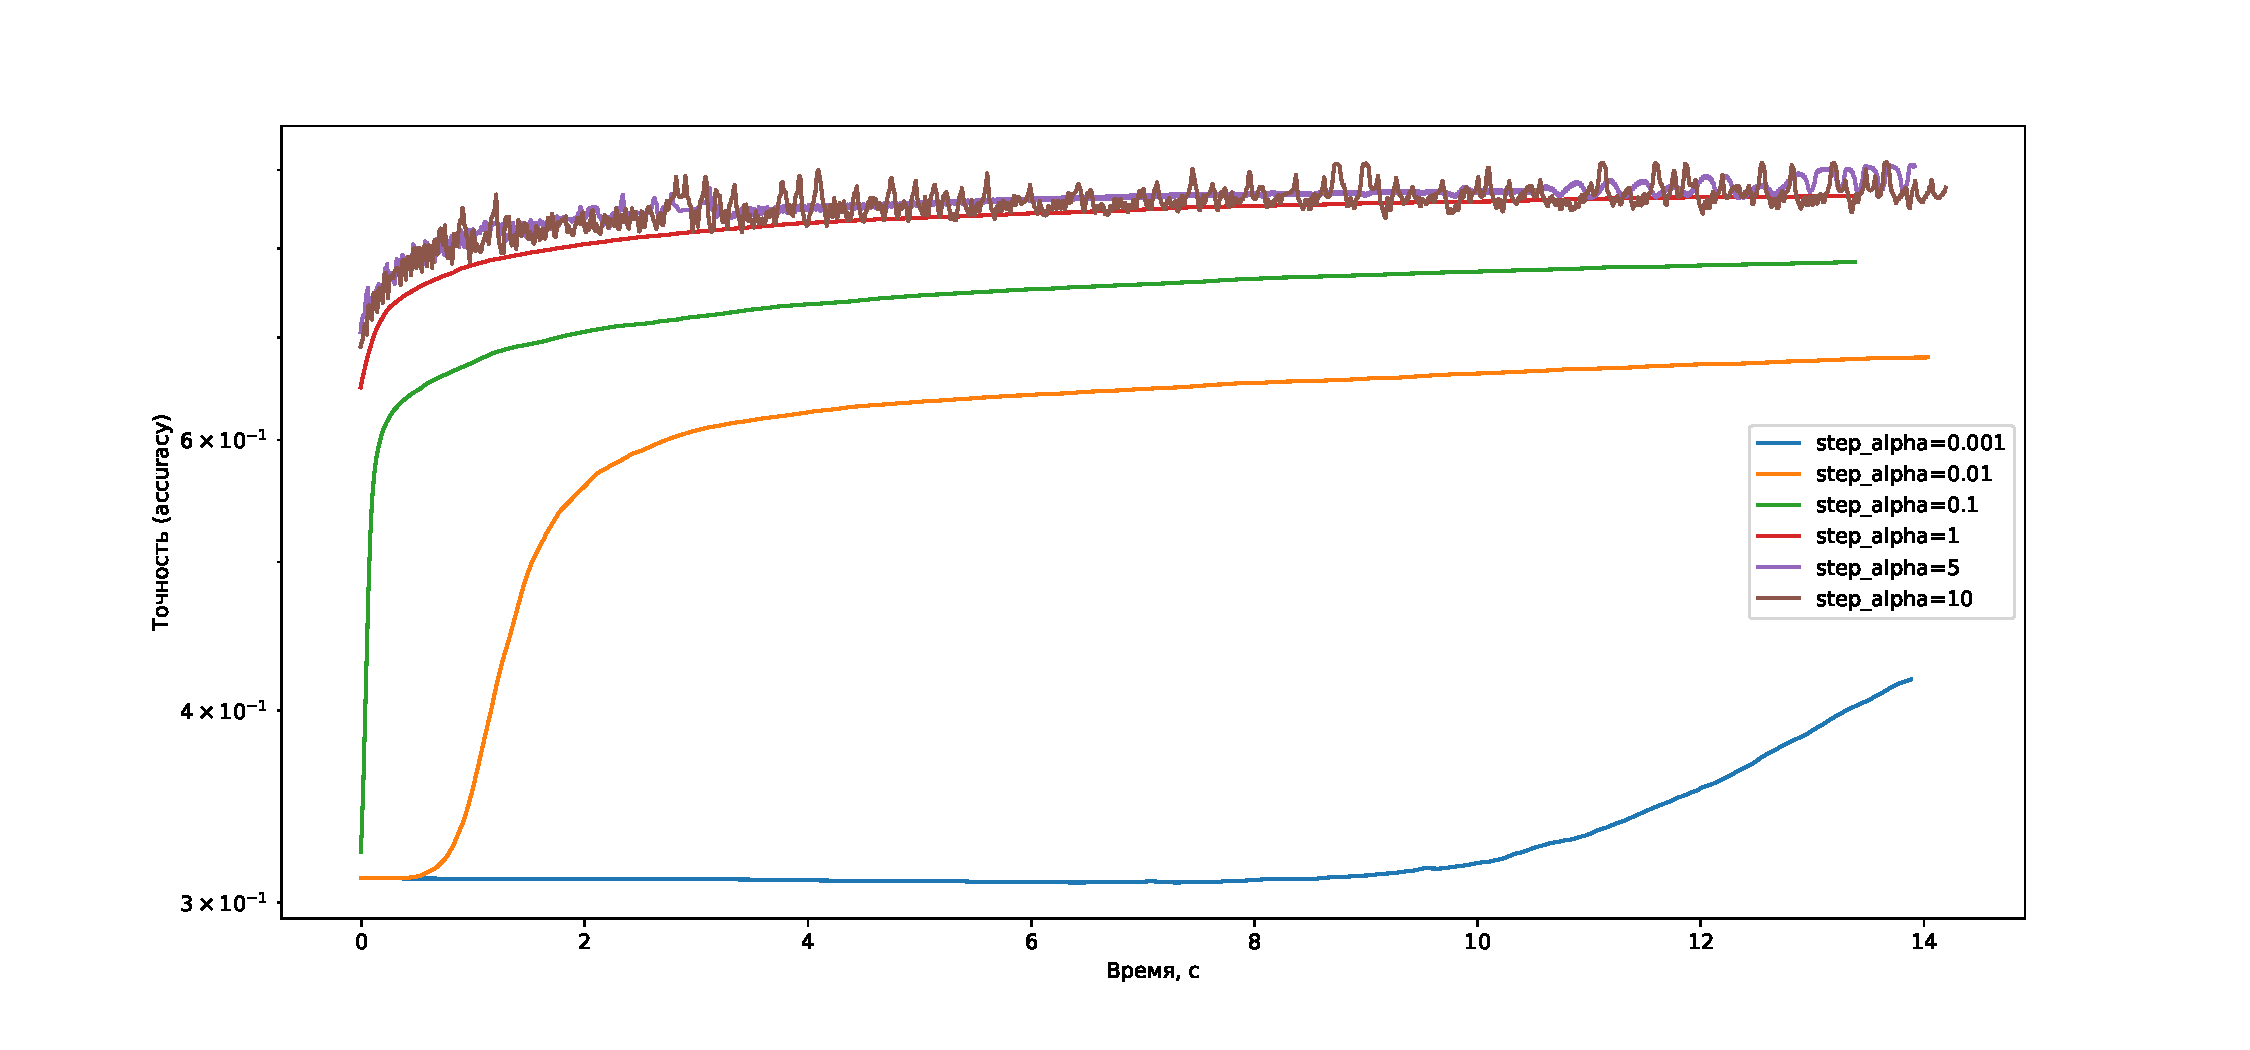
\includegraphics[width=0.5\textwidth, height=0.25\textheight]{../graphs/exp1_accuracy_GD_alpha_time_beta=0,001.pdf}
                            
                            \caption{Зависимость значения функции потерь от итерации метода стохастического градиентного спуска} \label{exp3:gd_func_iter}
                            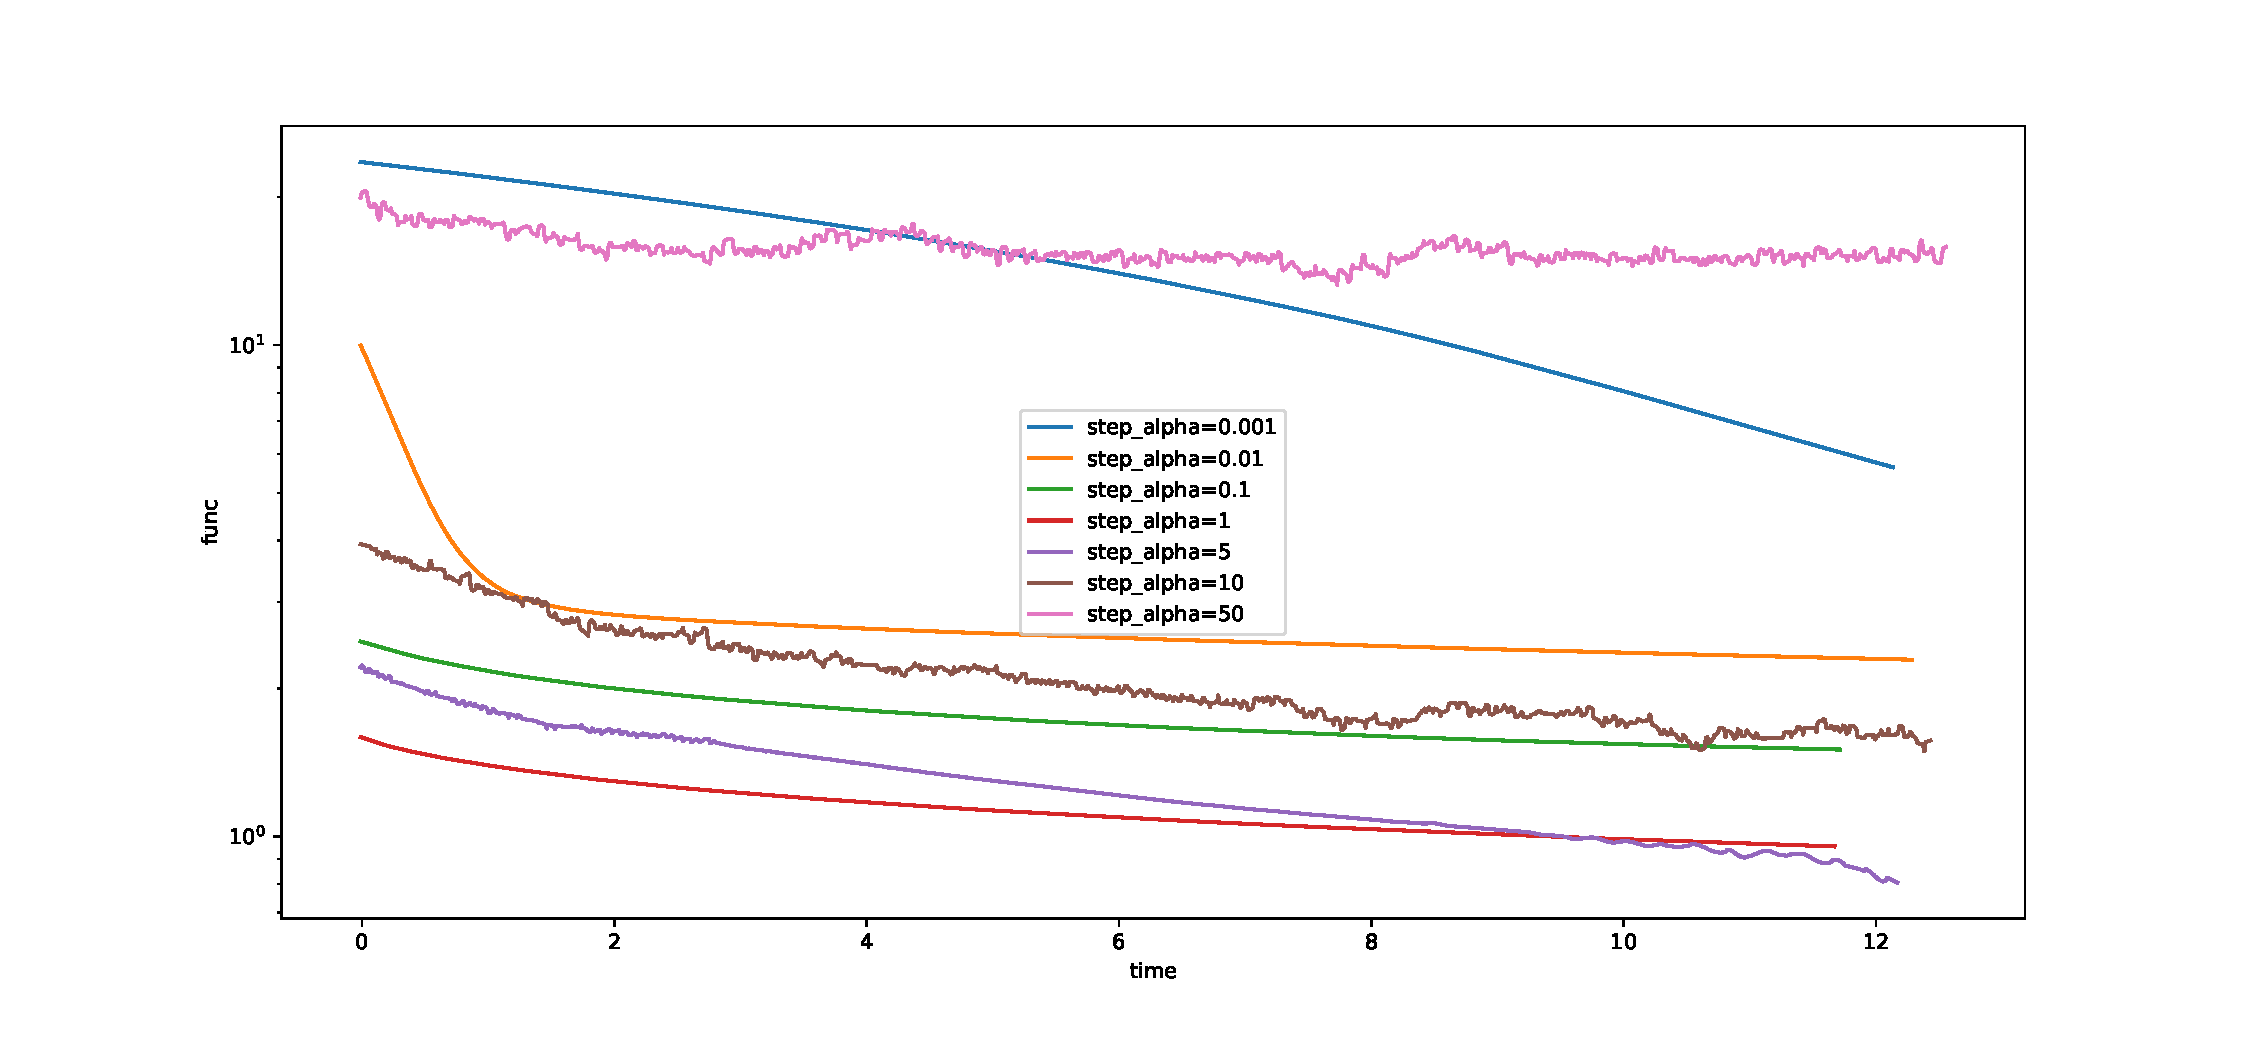
\includegraphics[width=0.5\textwidth, height=0.25\textheight]{../graphs/exp1_func_GD_alpha_time_beta=0,001.pdf}
                            
                            \caption{Зависимость значения точности (accuracy) от итерации метода стохастического градиентного спуска} \label{exp3:gd_acc_iter}
                            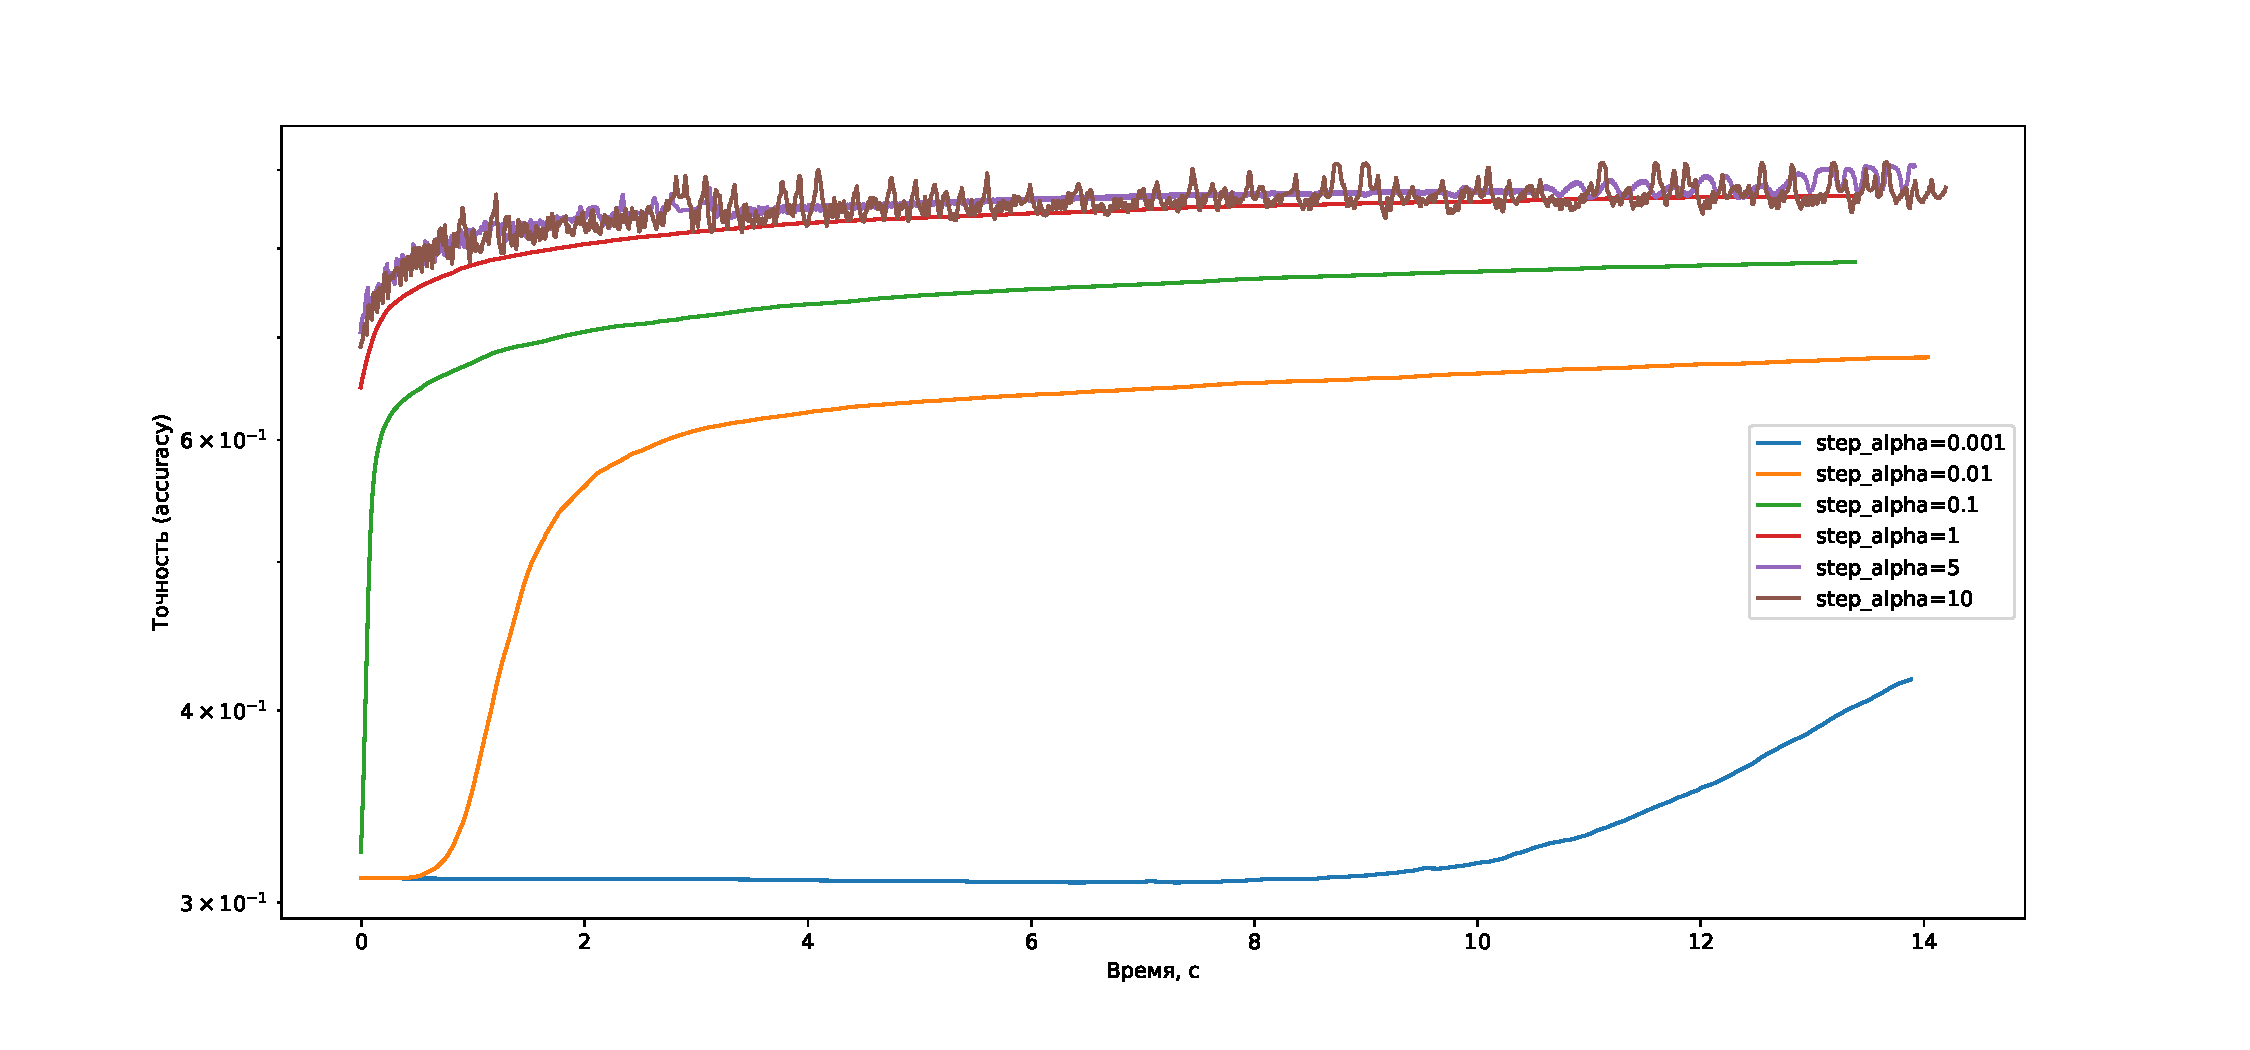
\includegraphics[width=0.5\textwidth, height=0.25\textheight]{../graphs/exp1_accuracy_GD_alpha_time_beta=0,001.pdf}
                        \end{center}
                    \end{multicols}
                \end{figure}
            
            
       \subsection{Исследование поведения стохастического градиентного спуска}
            Обновления весов модели при использовании стохастического градиетного спуска происходит по следующей формуле:
            \begin{equation}\label{exp1:weight_upd_sgd}
            w_t = w_{t-1} - \frac{\alpha}{t^\beta} \times \frac{1}{|I|} \times \sum_{i \in I}\nabla_{w}\mathcal{L}(x_i, y_i|w_{t-1}),
            \end{equation}
            где $t$ - номер итерации, $\beta$ - \textbf{step\_beta}, $I$ - некоторое подможнество индексов тренировочной выборки,  $\nabla_{w}\mathcal{L}(x_i, y_i|w_{t-1})$ - градиент функции потерь.
            \subsubsection{Параметр размера шага \textbf{step\_alpha}}
            Параметр \textbf{step\_alpha $(\alpha)$} используется в стохастическом градиентном спуске при обновлении весов в формуле \ref{exp1:weight_upd_sgd}.
            Рассмотрим следующие зависимости при разных значениях параметра \textbf{step\_alpha}:
            \begin{enumerate}\label{exp:dependencies_sgd}
                \item зависимость значения функции потерь от реального времени работы метода
                \item зависимость точности (accuracy) от реального времени работы метода
                \item зависимость значения функции потерь от эпохи метода
                \item зависимость точности (accuracy) от эпохи метода
            \end{enumerate}
            Соответствующие графики приведены на: рис. \ref{exp1:sgd_func_time}, \ref{exp1:sgd_acc_time}, \ref{exp1:sgd_func_iter}, \ref{exp1:sgd_acc_iter}.
            
            \begin{figure}[H] \label{exp1}
                \begin{multicols}{2}
                    \begin{center}
                        \caption{Зависимость значения функции потерь от реального времени работы градиентного спуска} \label{exp1:sgd_func_time}
                        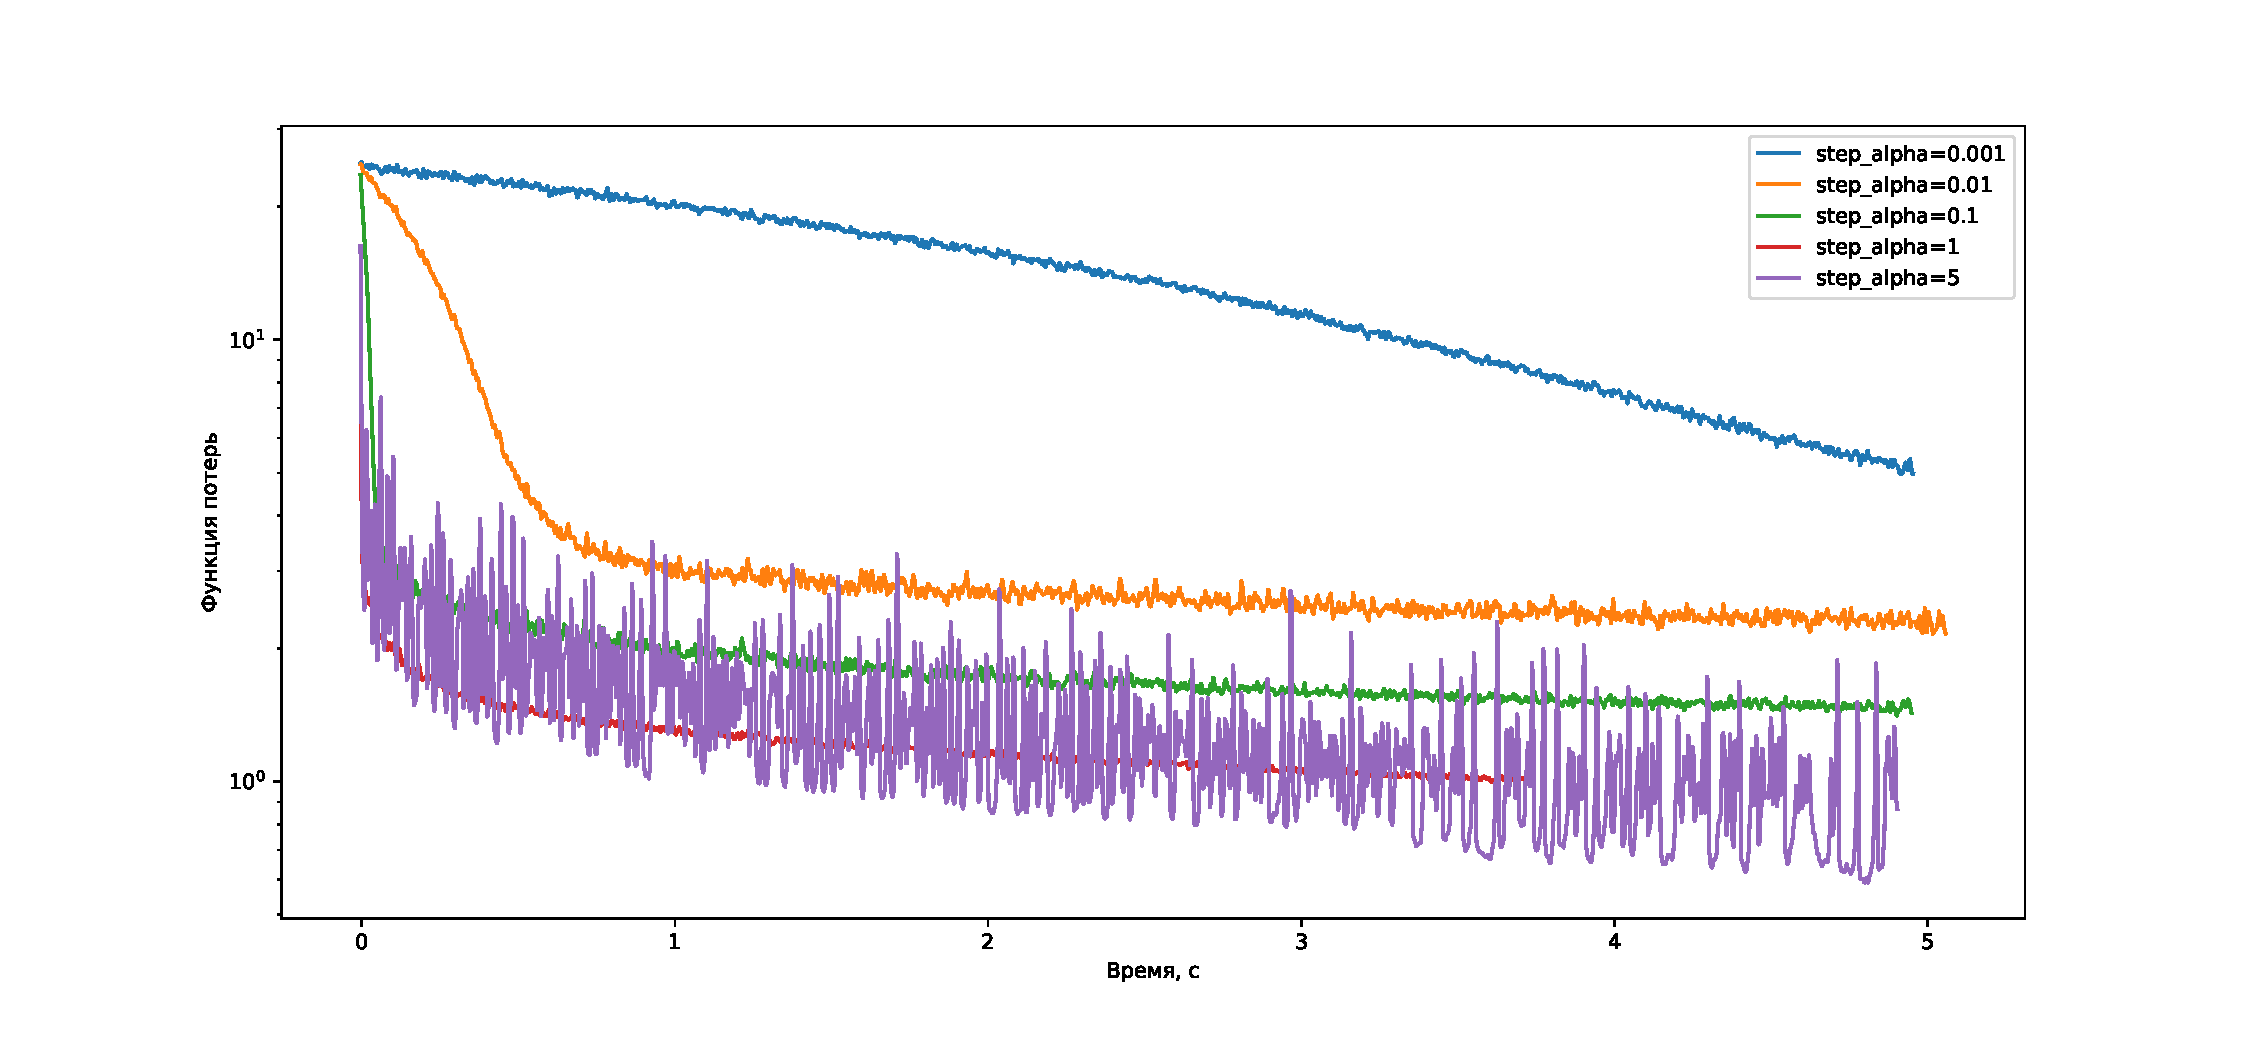
\includegraphics[width=0.5\textwidth, height=0.25\textheight]{../graphs/exp1_func_SGD_alpha_time_beta=0,001_bs=4096.pdf}
                        
                        \caption{Зависимость значения точности (accuracy) от реального времени работы градиентного спуска} \label{exp1:sgd_acc_time}
                        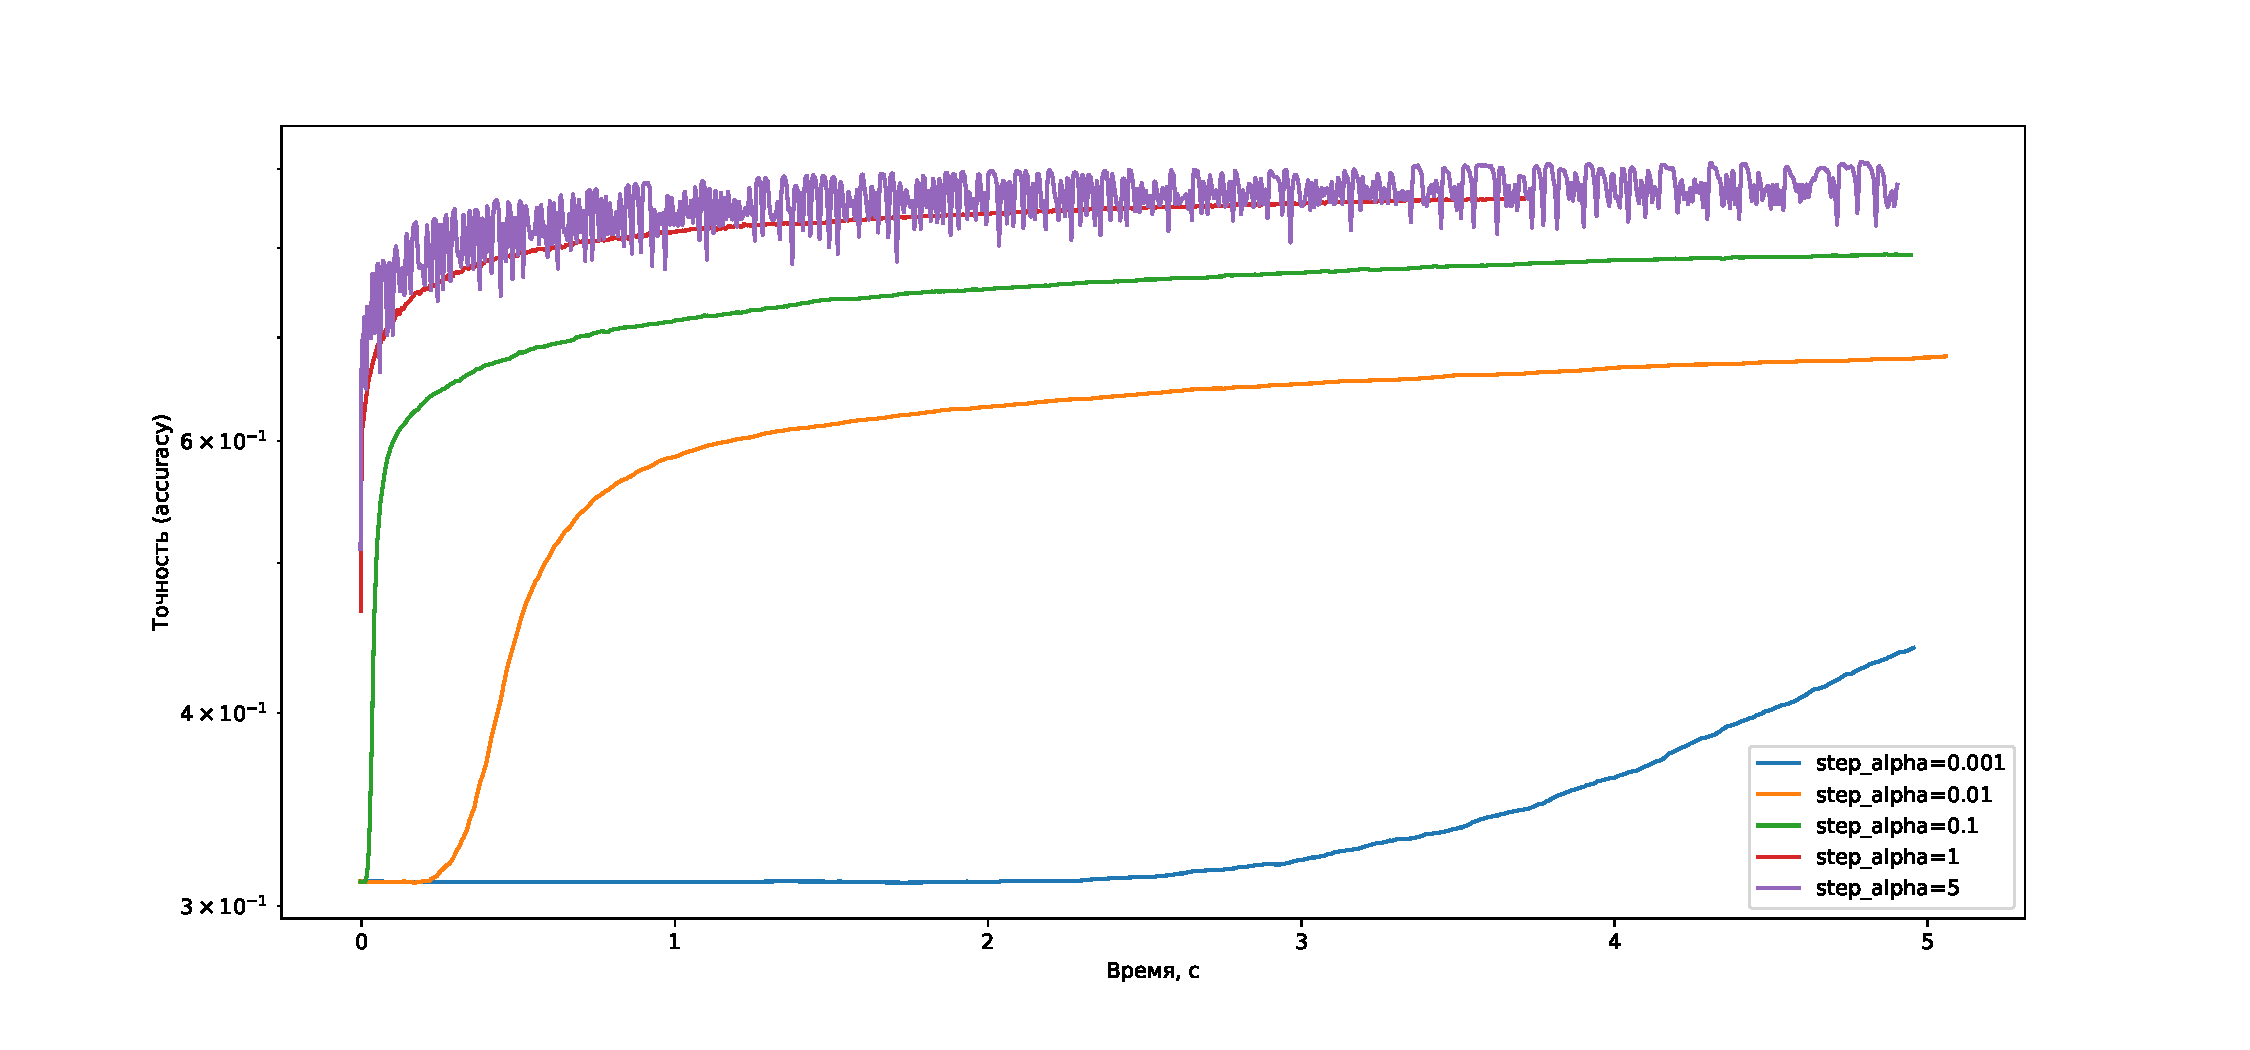
\includegraphics[width=0.5\textwidth, height=0.25\textheight]{../graphs/exp1_accuracy_SGD_alpha_time_beta=0,001_bs=4096.pdf}
                        
                        \caption{Зависимость значения функции потерь от эпохи метода градиентного спуска} \label{exp1:sgd_func_iter}
                        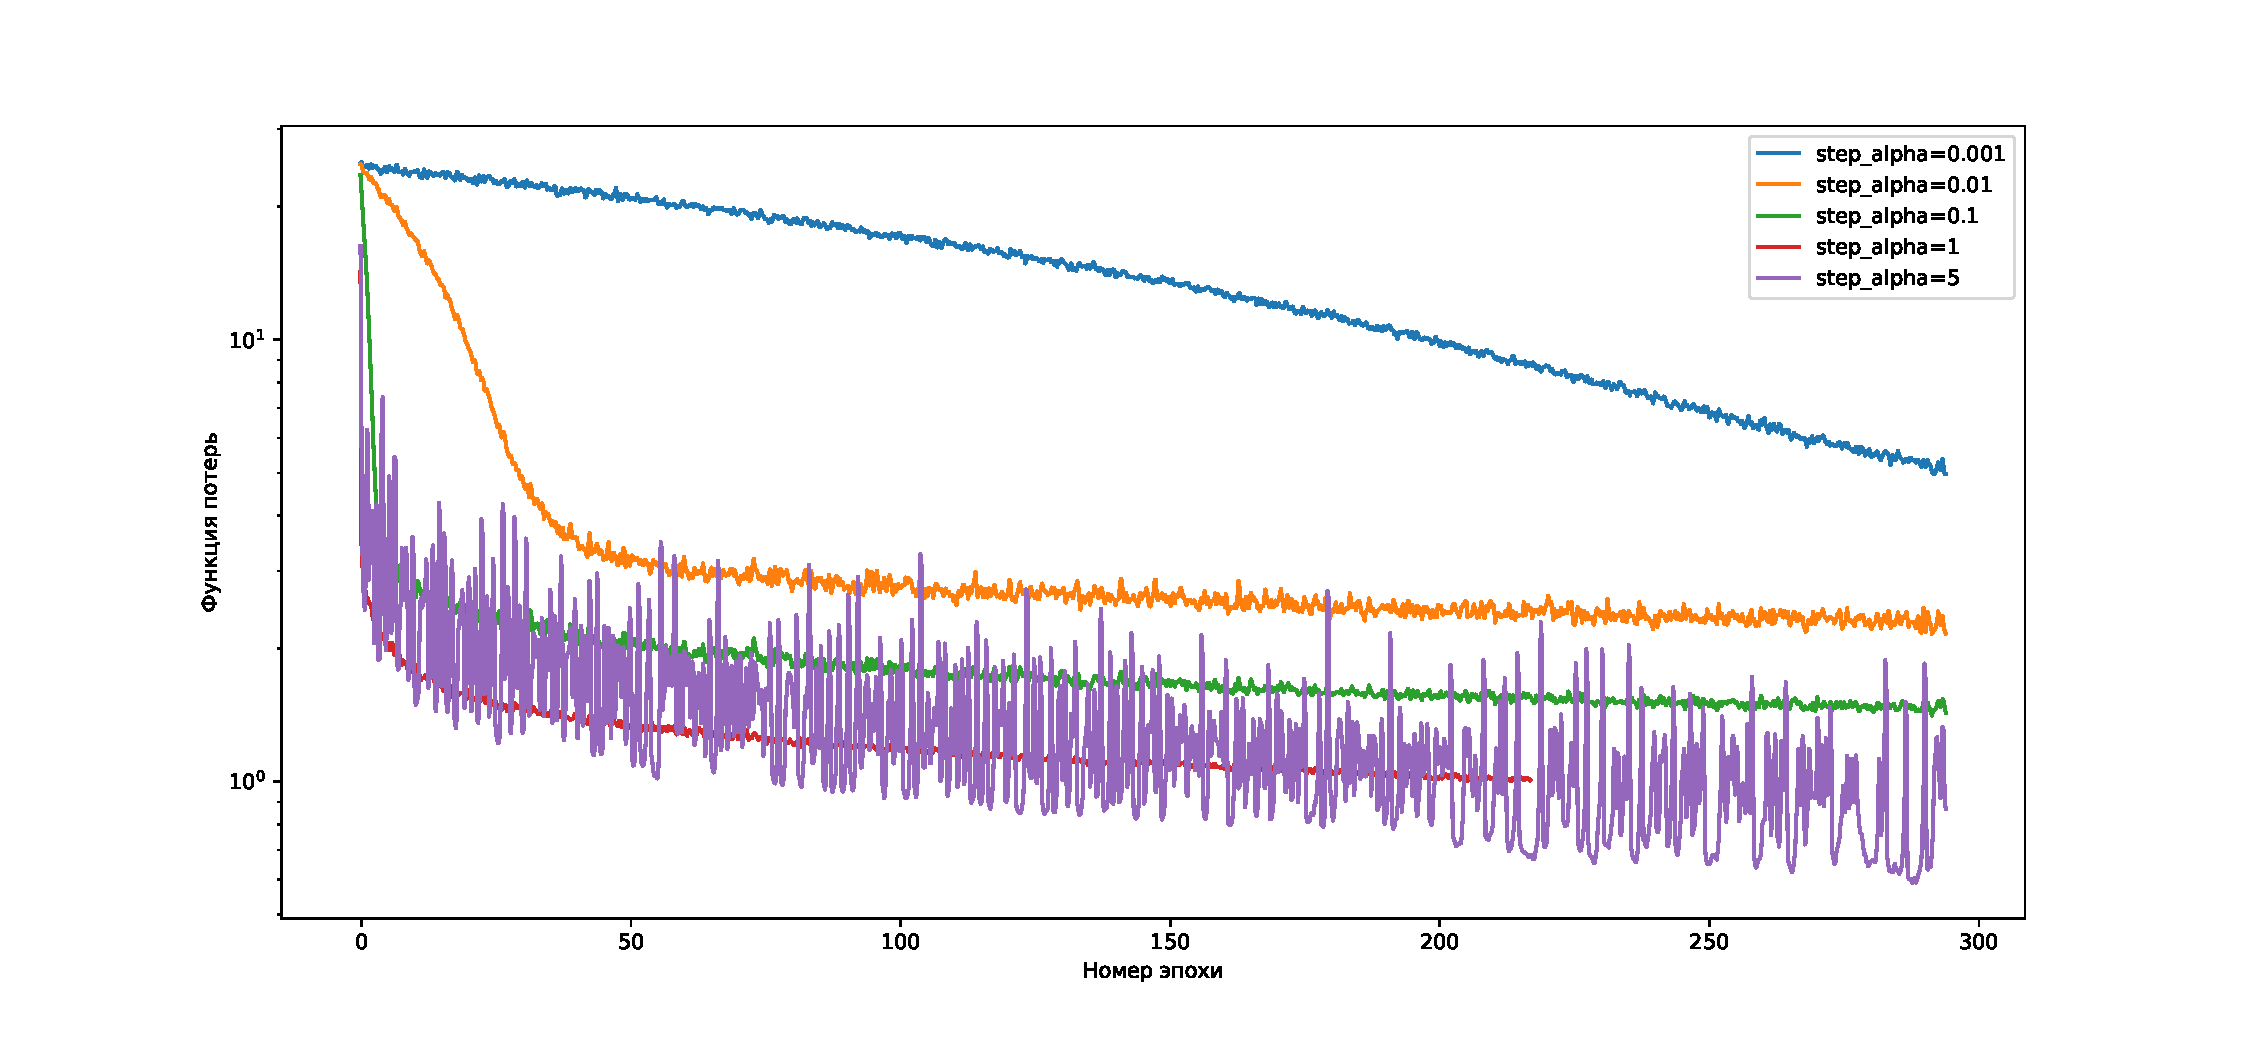
\includegraphics[width=0.5\textwidth, height=0.25\textheight]{../graphs/exp1_func_SGD_alpha_epoch_num_beta=0,001_bs=4096.pdf}
                        
                        \caption{Зависимость значения точности (accuracy) от эпохи метода градиентного спуска} \label{exp1:sgd_acc_iter}
                        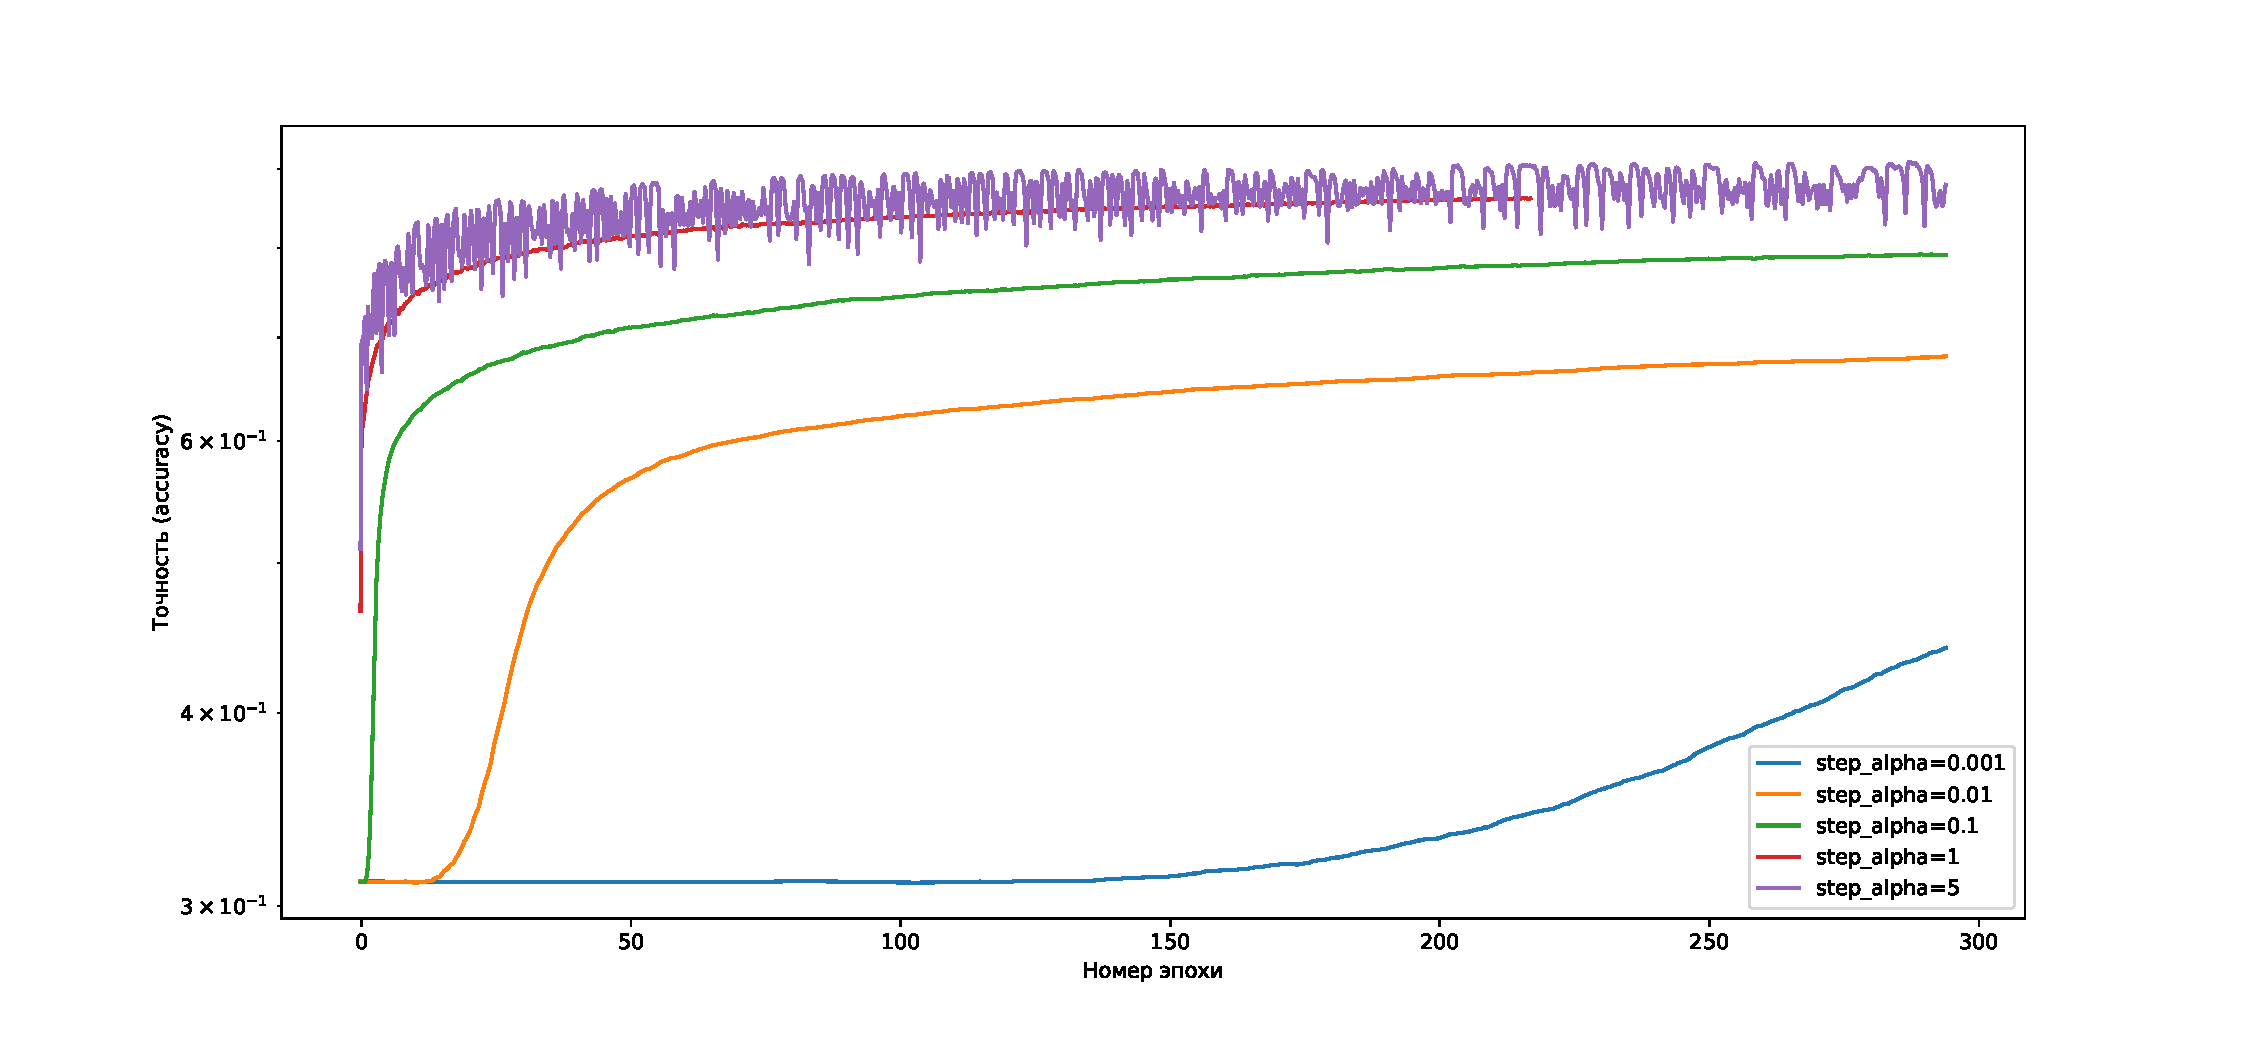
\includegraphics[width=0.5\textwidth, height=0.25\textheight]{../graphs/exp1_accuracy_SGD_alpha_epoch_num_beta=0,001_bs=4096.pdf}
                    \end{center}
                \end{multicols}
            \end{figure}
            На графиках просматривается аналогичная ситуация, что и с градиентным спуском: при значениях \textbf{step\_alpha}, близких к 0 возникает эффект недообучения, а при  больших - появляется нестабильность кривой обучения, но есть точки, в которых достигается наивысшая точность. В таком случае можно производить сохранение весов модели на итерации со значением наилучшей точности. Возможно, такой метод поможет справиться с нестабильностью.
            
            \subsubsection{Параметр размера шага step\_beta}
            Параметр \textbf{step\_beta $(\beta)$} используется в градиентном спуске при обновлении весов в формуле \ref{exp1:weight_upd}.
            Аналогично предыдущему пункту рассмотрим зависимости из \ref{exp:dependencies_sgd} при разных значениях параметра \textbf{step\_beta} и проанализруем соответсвующие графики, представленные на рис. \ref{exp2:sgd_func_time}, \ref{exp2:sgd_acc_time}, \ref{exp2:sgd_func_iter}, \ref{exp2:sgd_acc_iter}.
            
            
            \begin{figure}[H] \label{exp1}
                \begin{multicols}{2}
                    \begin{center}
                        \caption{Зависимость значения функции потерь от реального времени работы градиентного спуска} \label{exp2:sgd_func_time}
                        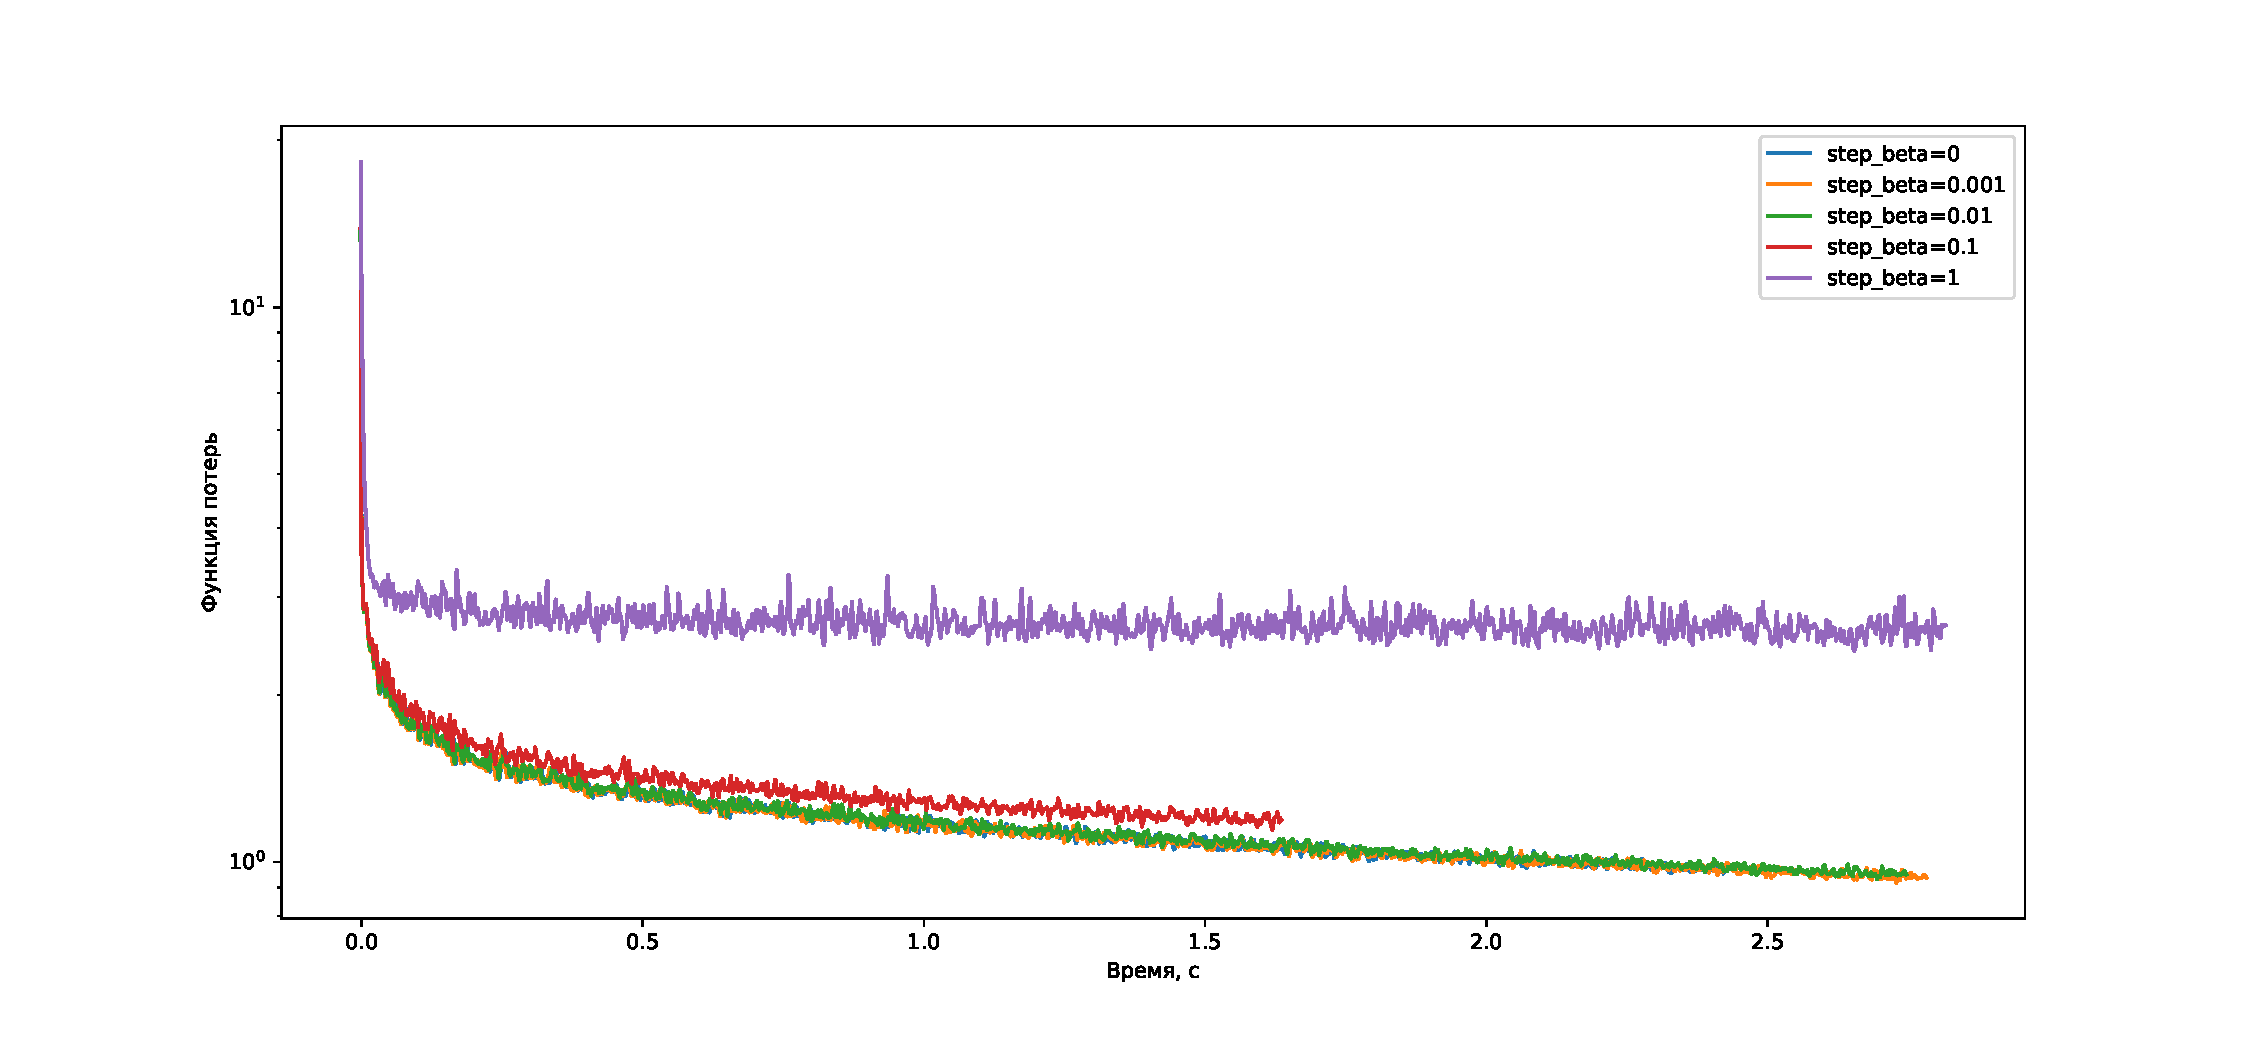
\includegraphics[width=0.5\textwidth, height=0.25\textheight]{../graphs/exp2_func_SGD_beta_time_alpha=1_bs=4096.pdf}
                        
                        \caption{Зависимость значения точности (accuracy) от реального времени работы градиентного спуска} \label{exp2:sgd_acc_time}
                        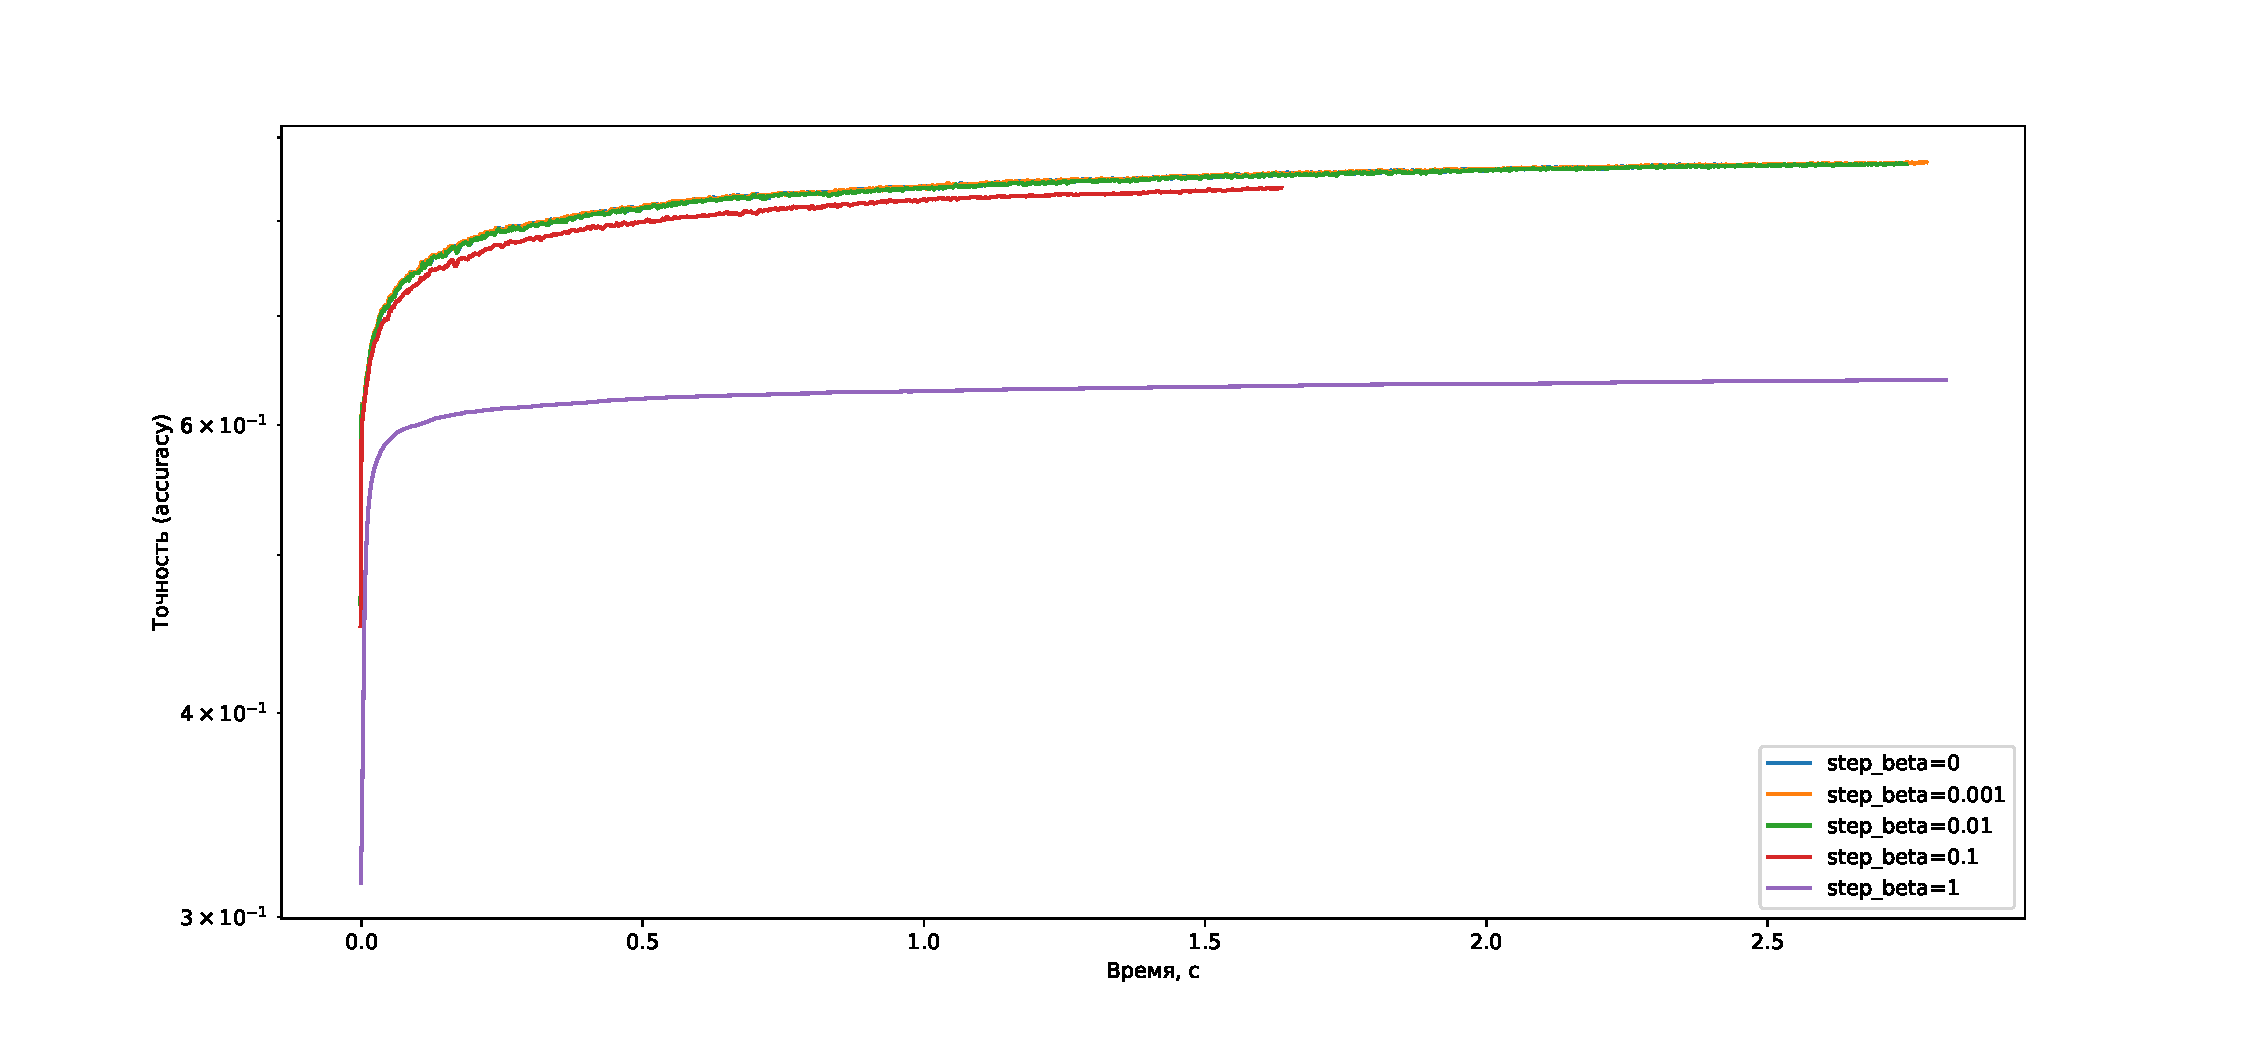
\includegraphics[width=0.5\textwidth, height=0.25\textheight]{../graphs/exp2_accuracy_SGD_beta_time_alpha=1_bs=4096.pdf}
                        
                        \caption{Зависимость значения функции потерь от эпохи метода градиентного спуска} \label{exp2:sgd_func_iter}
                        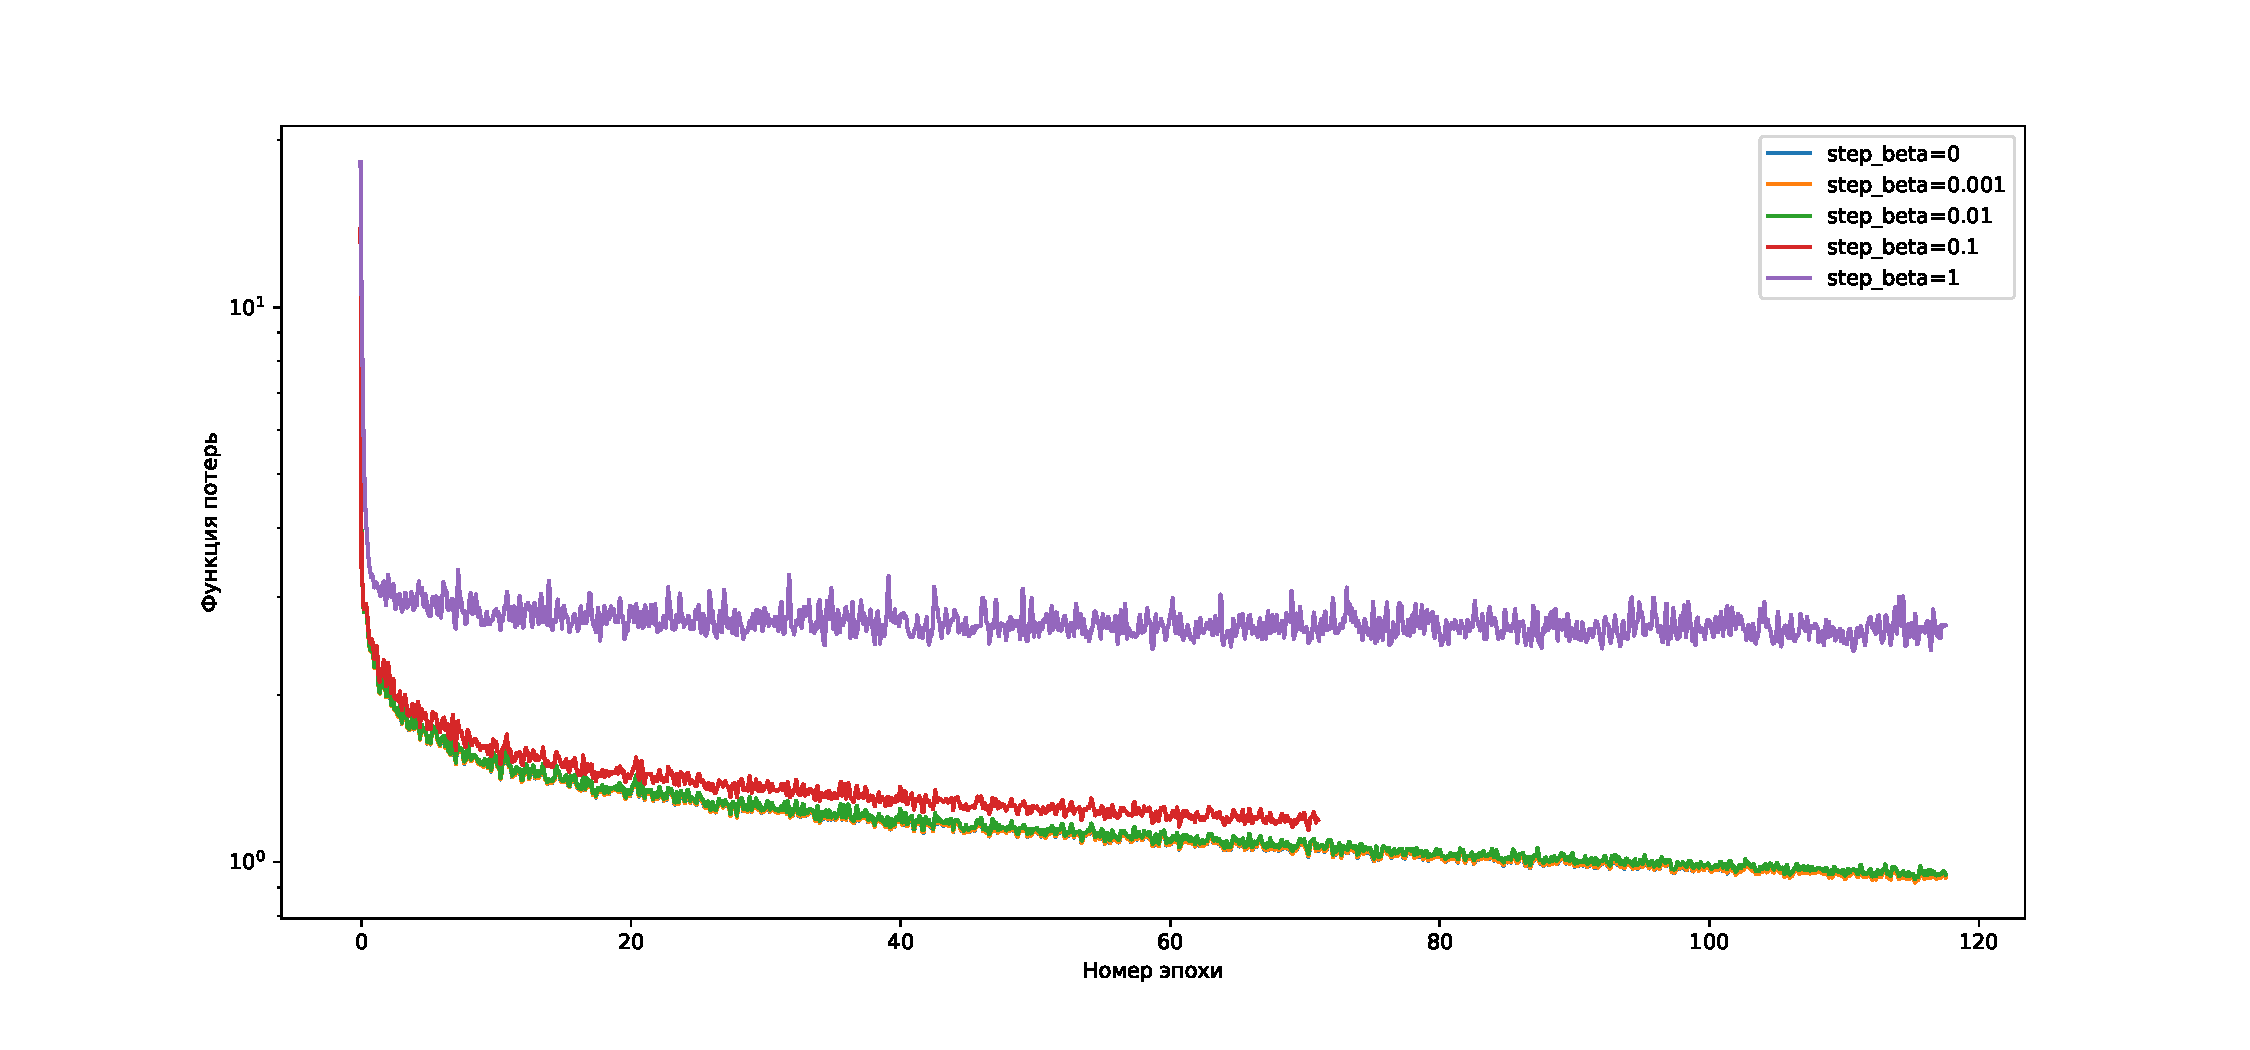
\includegraphics[width=0.5\textwidth, height=0.25\textheight]{../graphs/exp2_func_SGD_beta_epoch_num_alpha=1_bs=4096.pdf}
                        
                        \caption{Зависимость значения точности (accuracy) от эпохи метода градиентного спуска} \label{exp2:sgd_acc_iter}
                        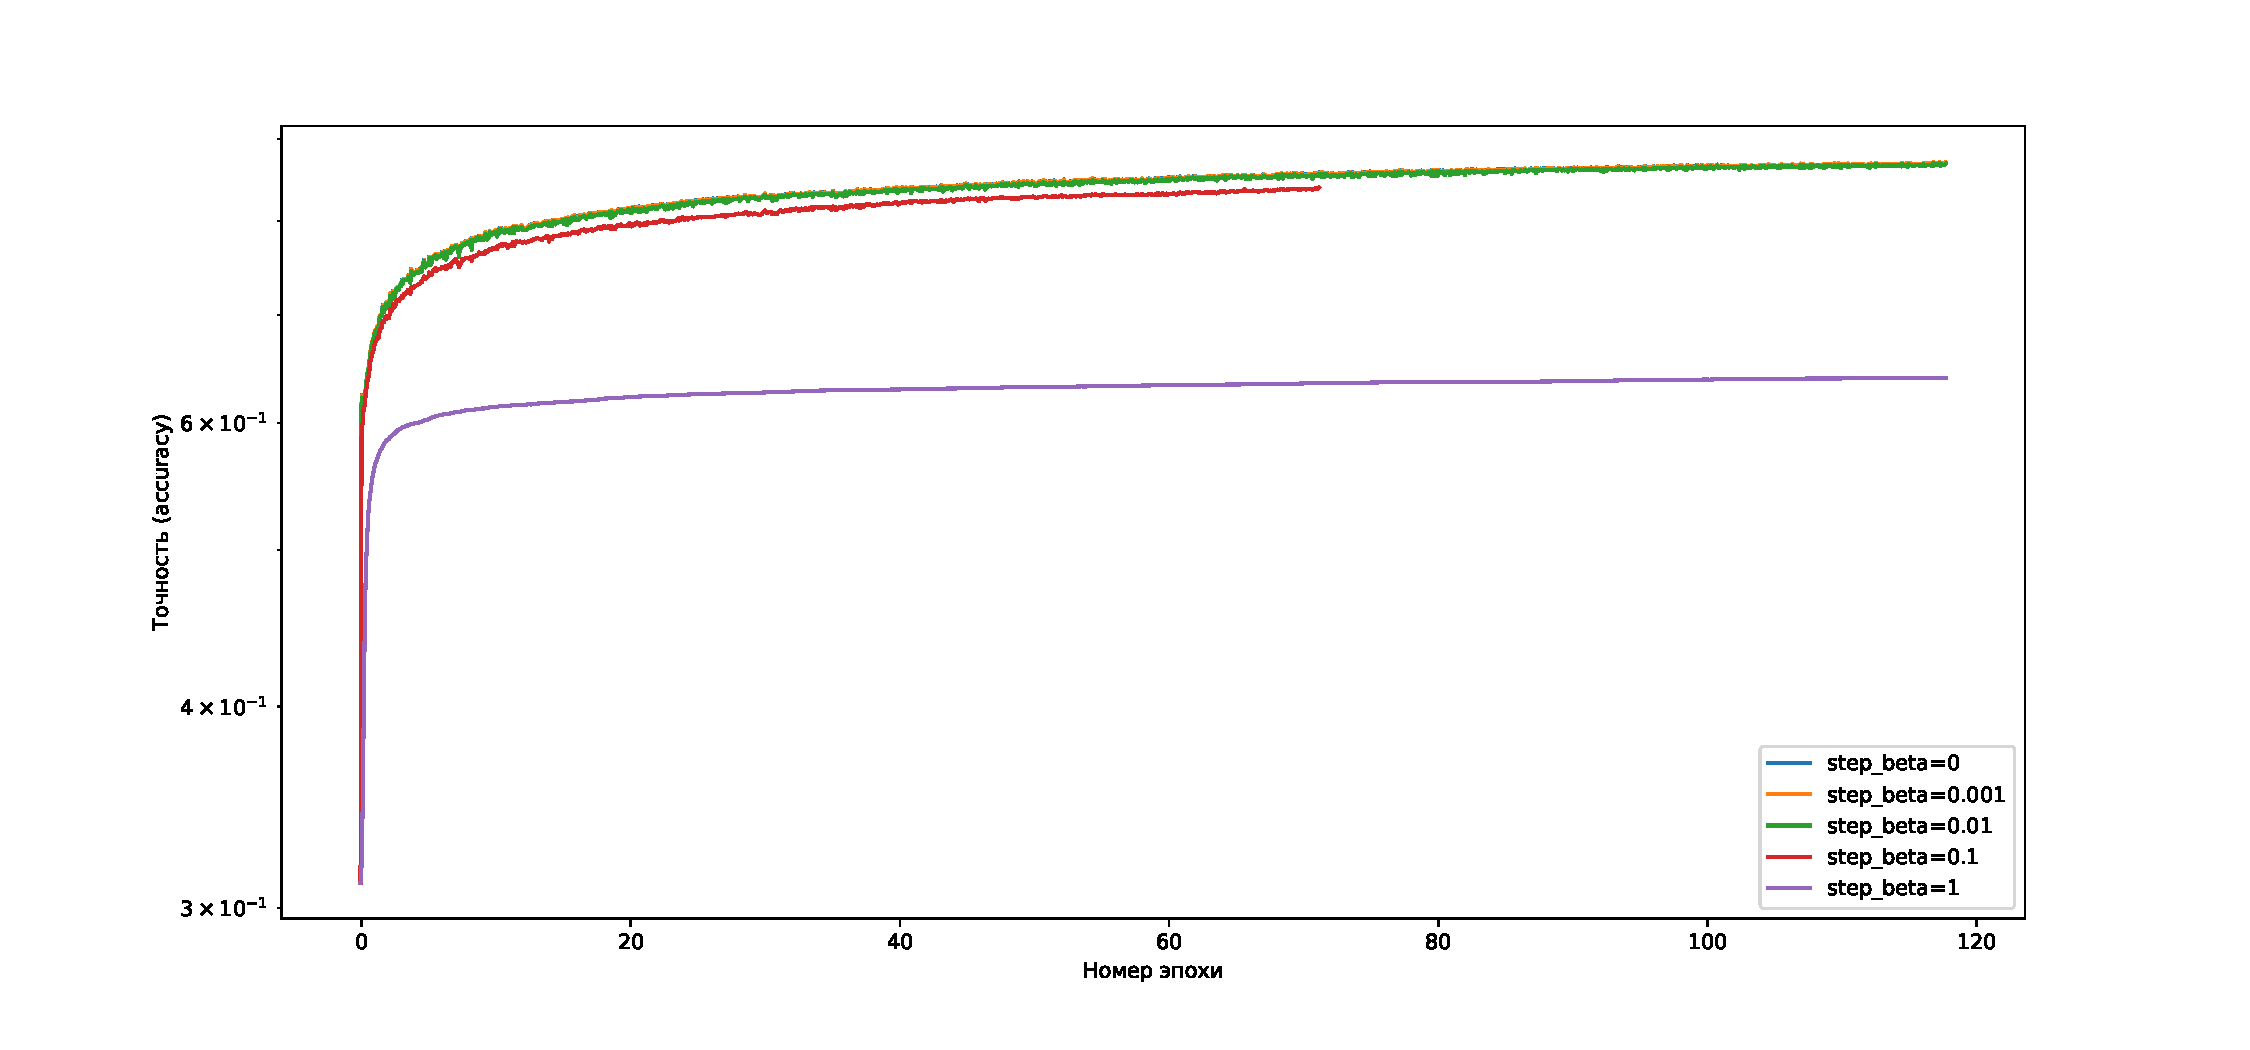
\includegraphics[width=0.5\textwidth, height=0.25\textheight]{../graphs/exp2_accuracy_SGD_beta_epoch_num_alpha=1_bs=4096.pdf}
                    \end{center}
                \end{multicols}
            \end{figure}
        
           Аналогично обычному градиентному спуску - с увелничением значения \textbf{step\_beta} увеличивается значение функции потерь и уменьшается точность (accuracy).
            
            \subsubsection{Размер подвыборки batch\_size}
                Размер подвыборки определяет количество элементов тренировочной выборки, которые будут использованы для подсчета градиента.
            
            Соответствующие графики приведены на рис. \ref{exp3:sgd_func_time}, \ref{exp3:sgd_acc_time}, \ref{exp3:sgd_func_iter}, \ref{exp3:sgd_acc_iter}.
            \begin{figure}[H] \label{exp1}
                \begin{multicols}{2}
                    \begin{center}
                        \caption{Зависимость значения функции потерь от реального времени работы градиентного спуска} \label{exp3:sgd_func_time}
                        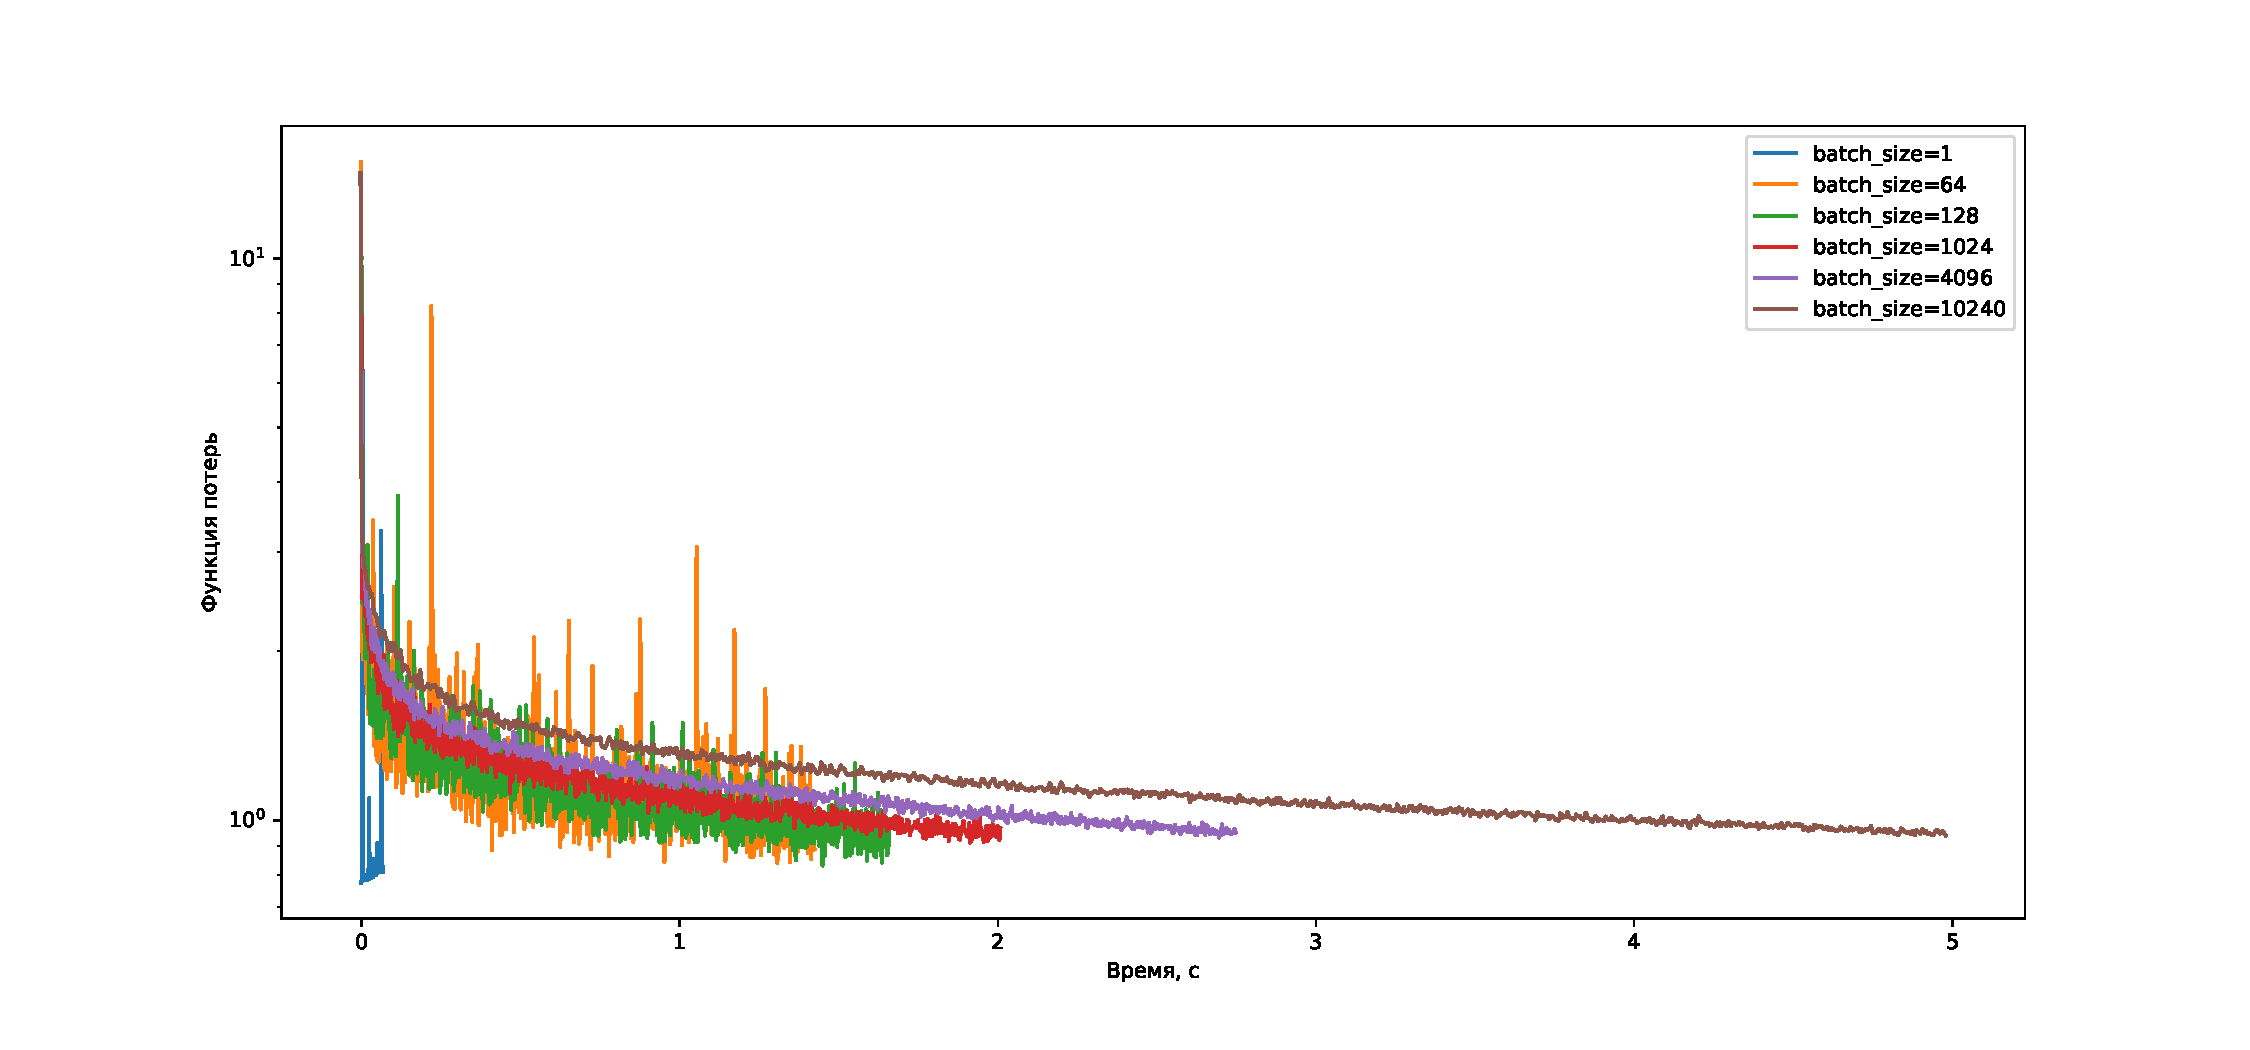
\includegraphics[width=0.5\textwidth, height=0.25\textheight]{../graphs/exp3_func_SGD_bs_time_alpha=1_beta=0,01.pdf}
                        
                        \caption{Зависимость значения точности (accuracy) от реального времени работы градиентного спуска} \label{exp3:sgd_acc_time}
                        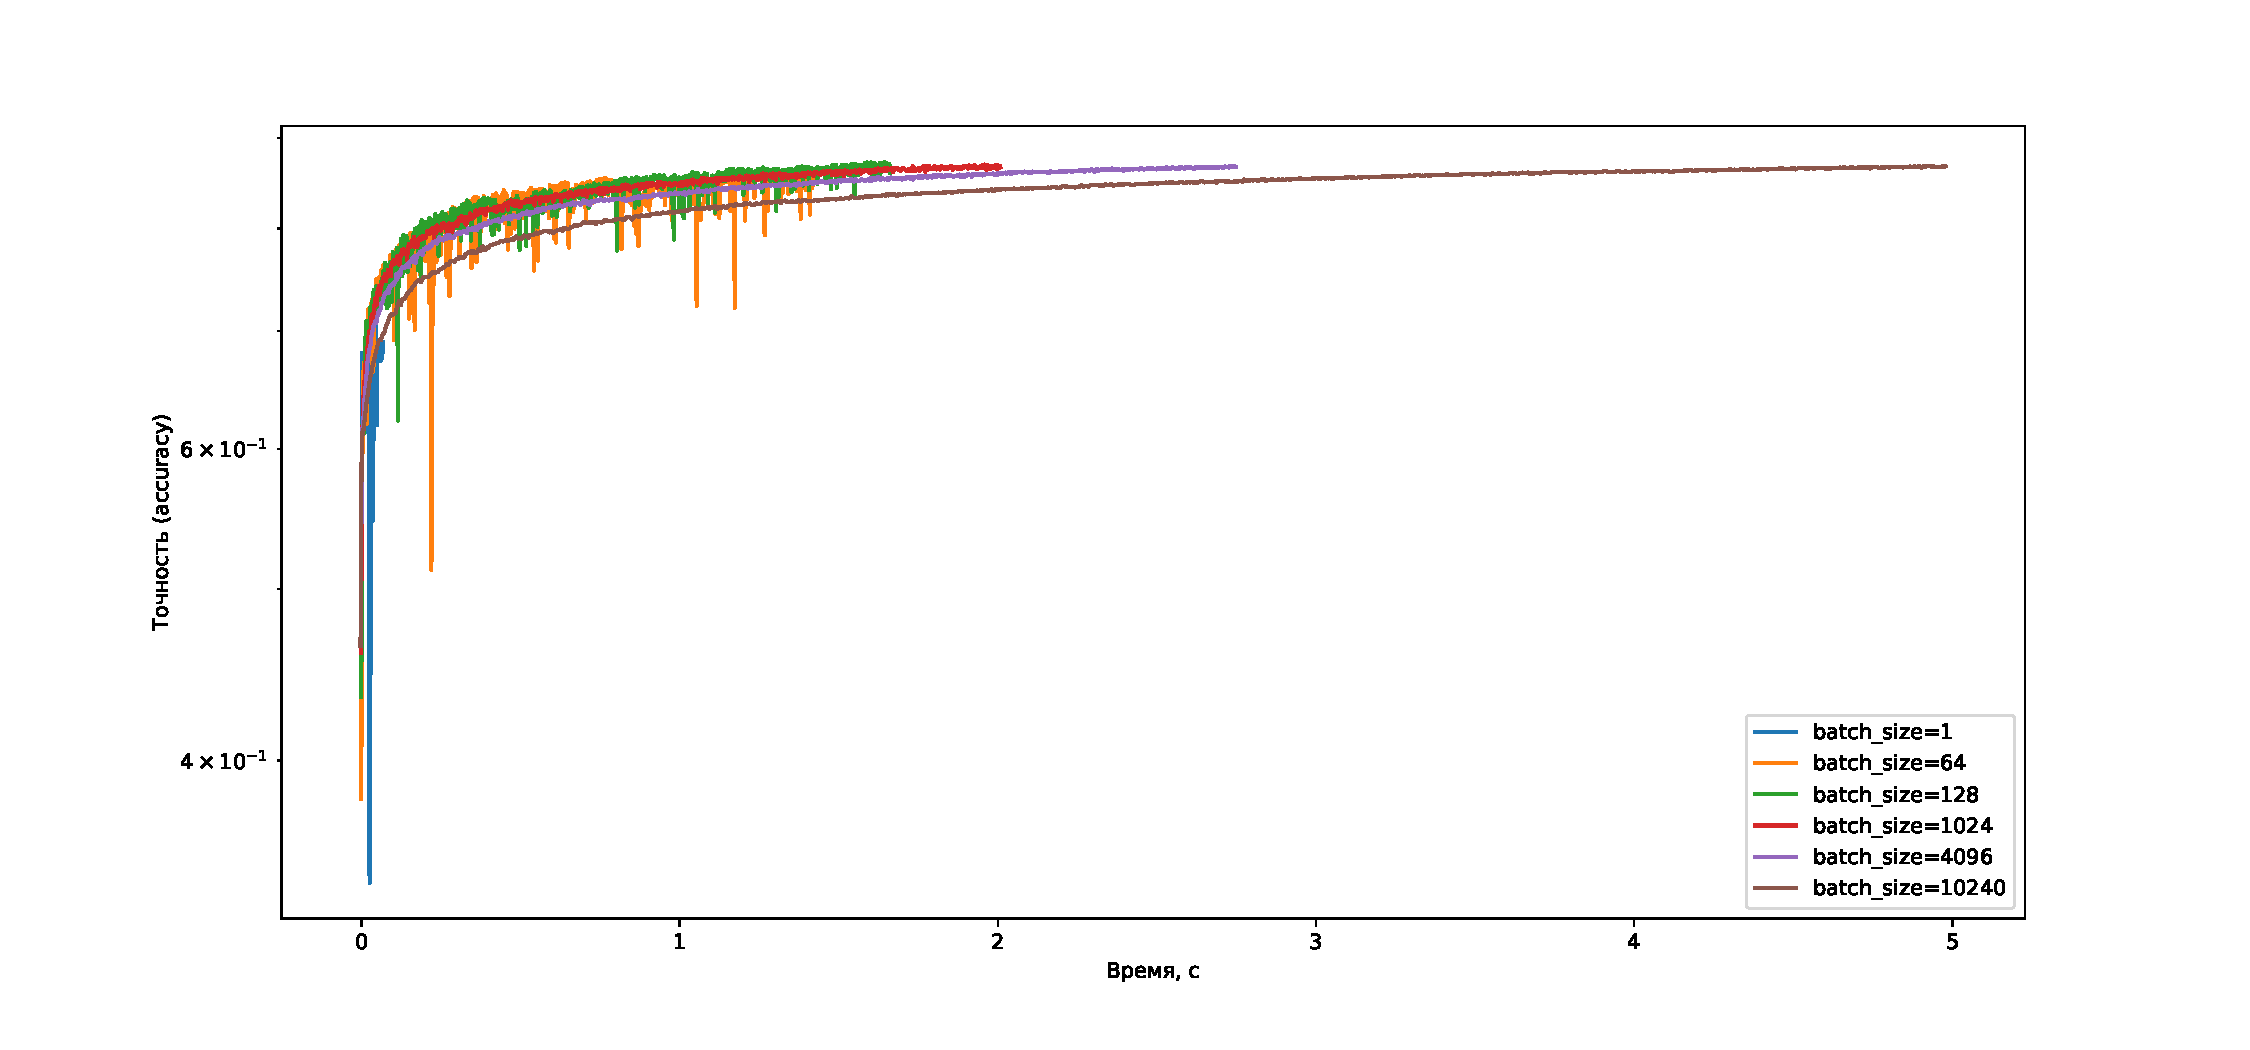
\includegraphics[width=0.5\textwidth, height=0.25\textheight]{../graphs/exp3_accuracy_SGD_bs_time_alpha=1_beta=0,01.pdf}
                        
                        \caption{Зависимость значения функции потерь от эпохи метода градиентного спуска} \label{exp3:sgd_func_iter}
                        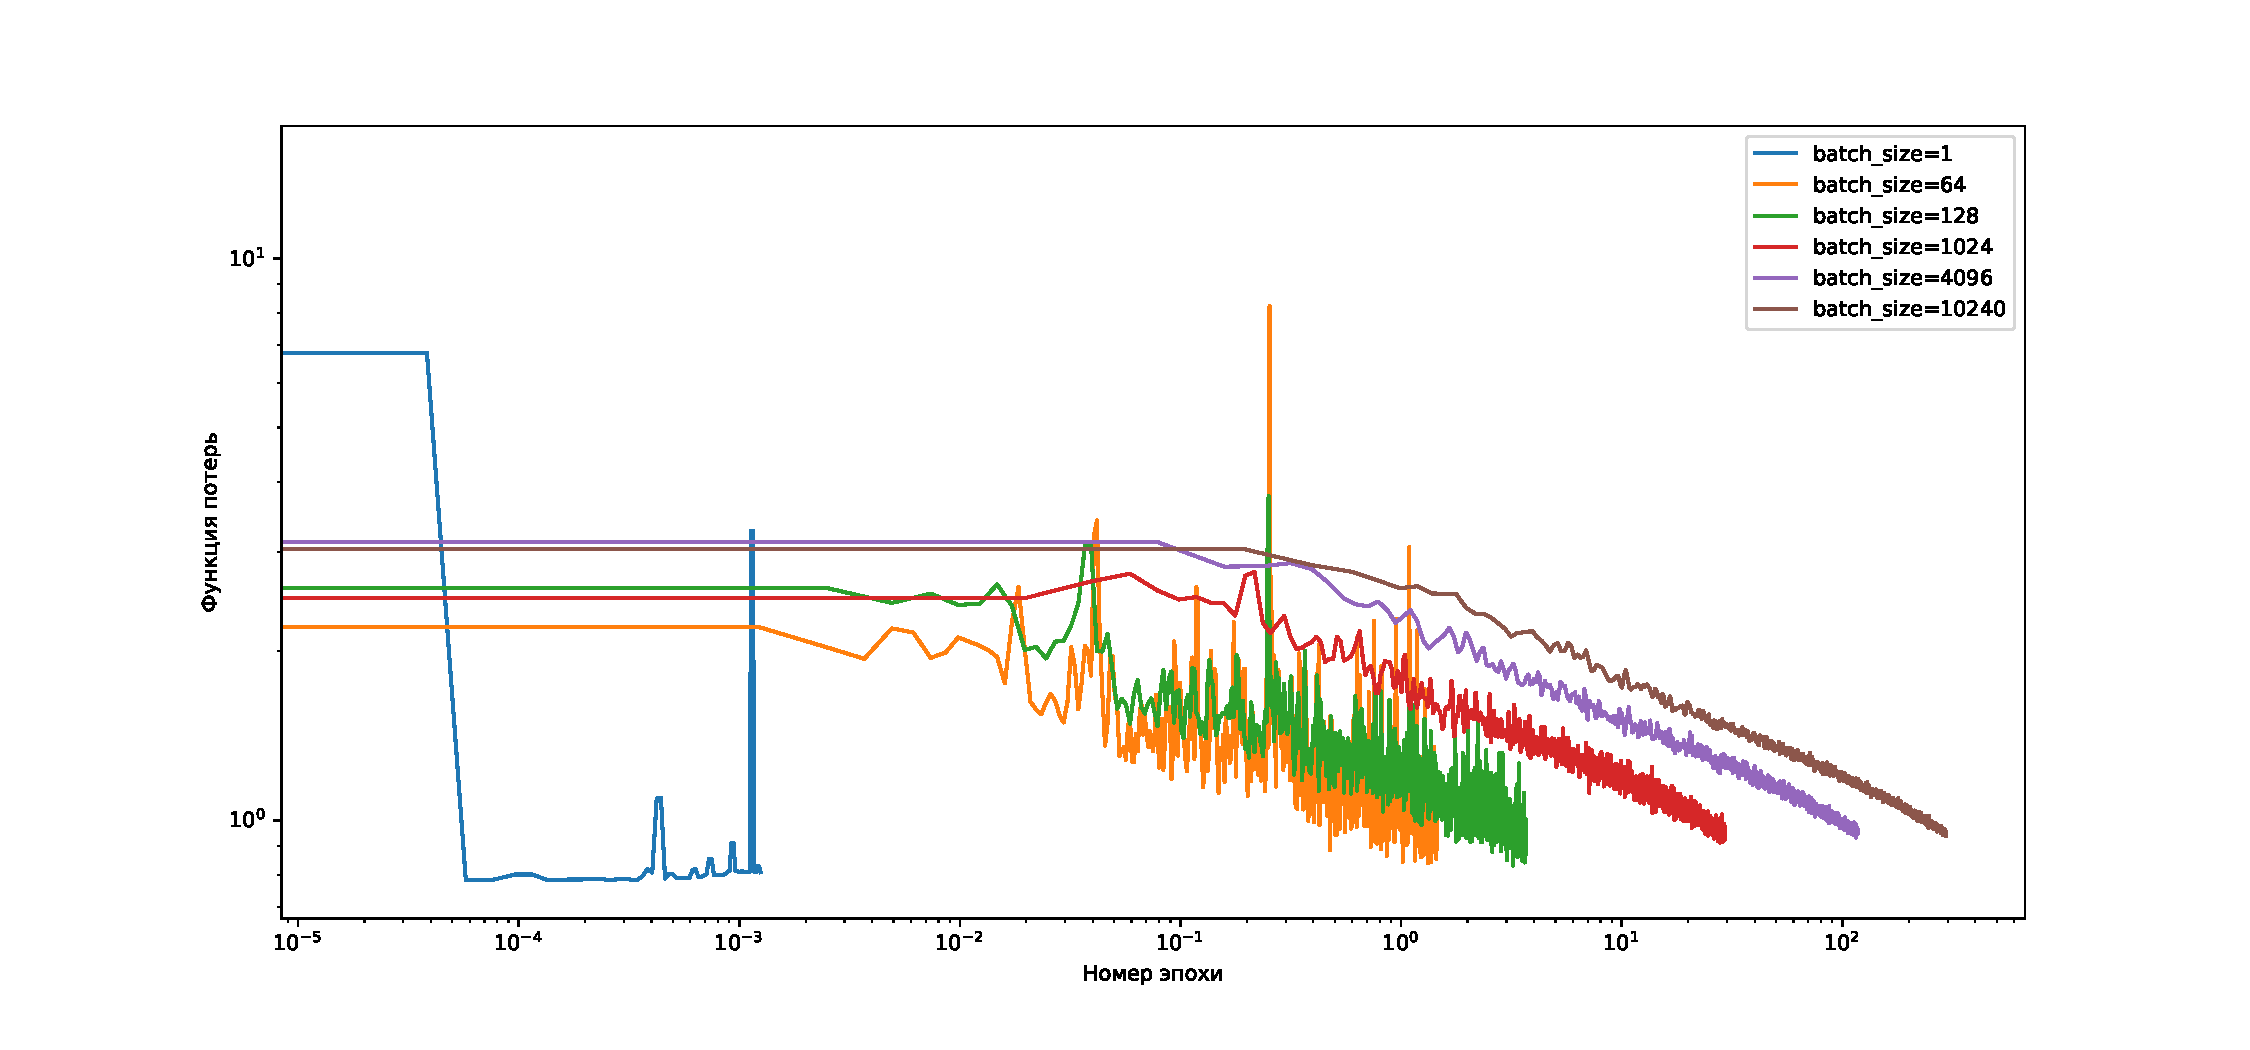
\includegraphics[width=0.5\textwidth, height=0.25\textheight]{../graphs/exp3_func_SGD_bs_epoch_num_alpha=1_beta=0,01.pdf}
                        
                        \caption{Зависимость значения точности (accuracy) от эпохи метода градиентного спуска} \label{exp3:sgd_acc_iter}
                        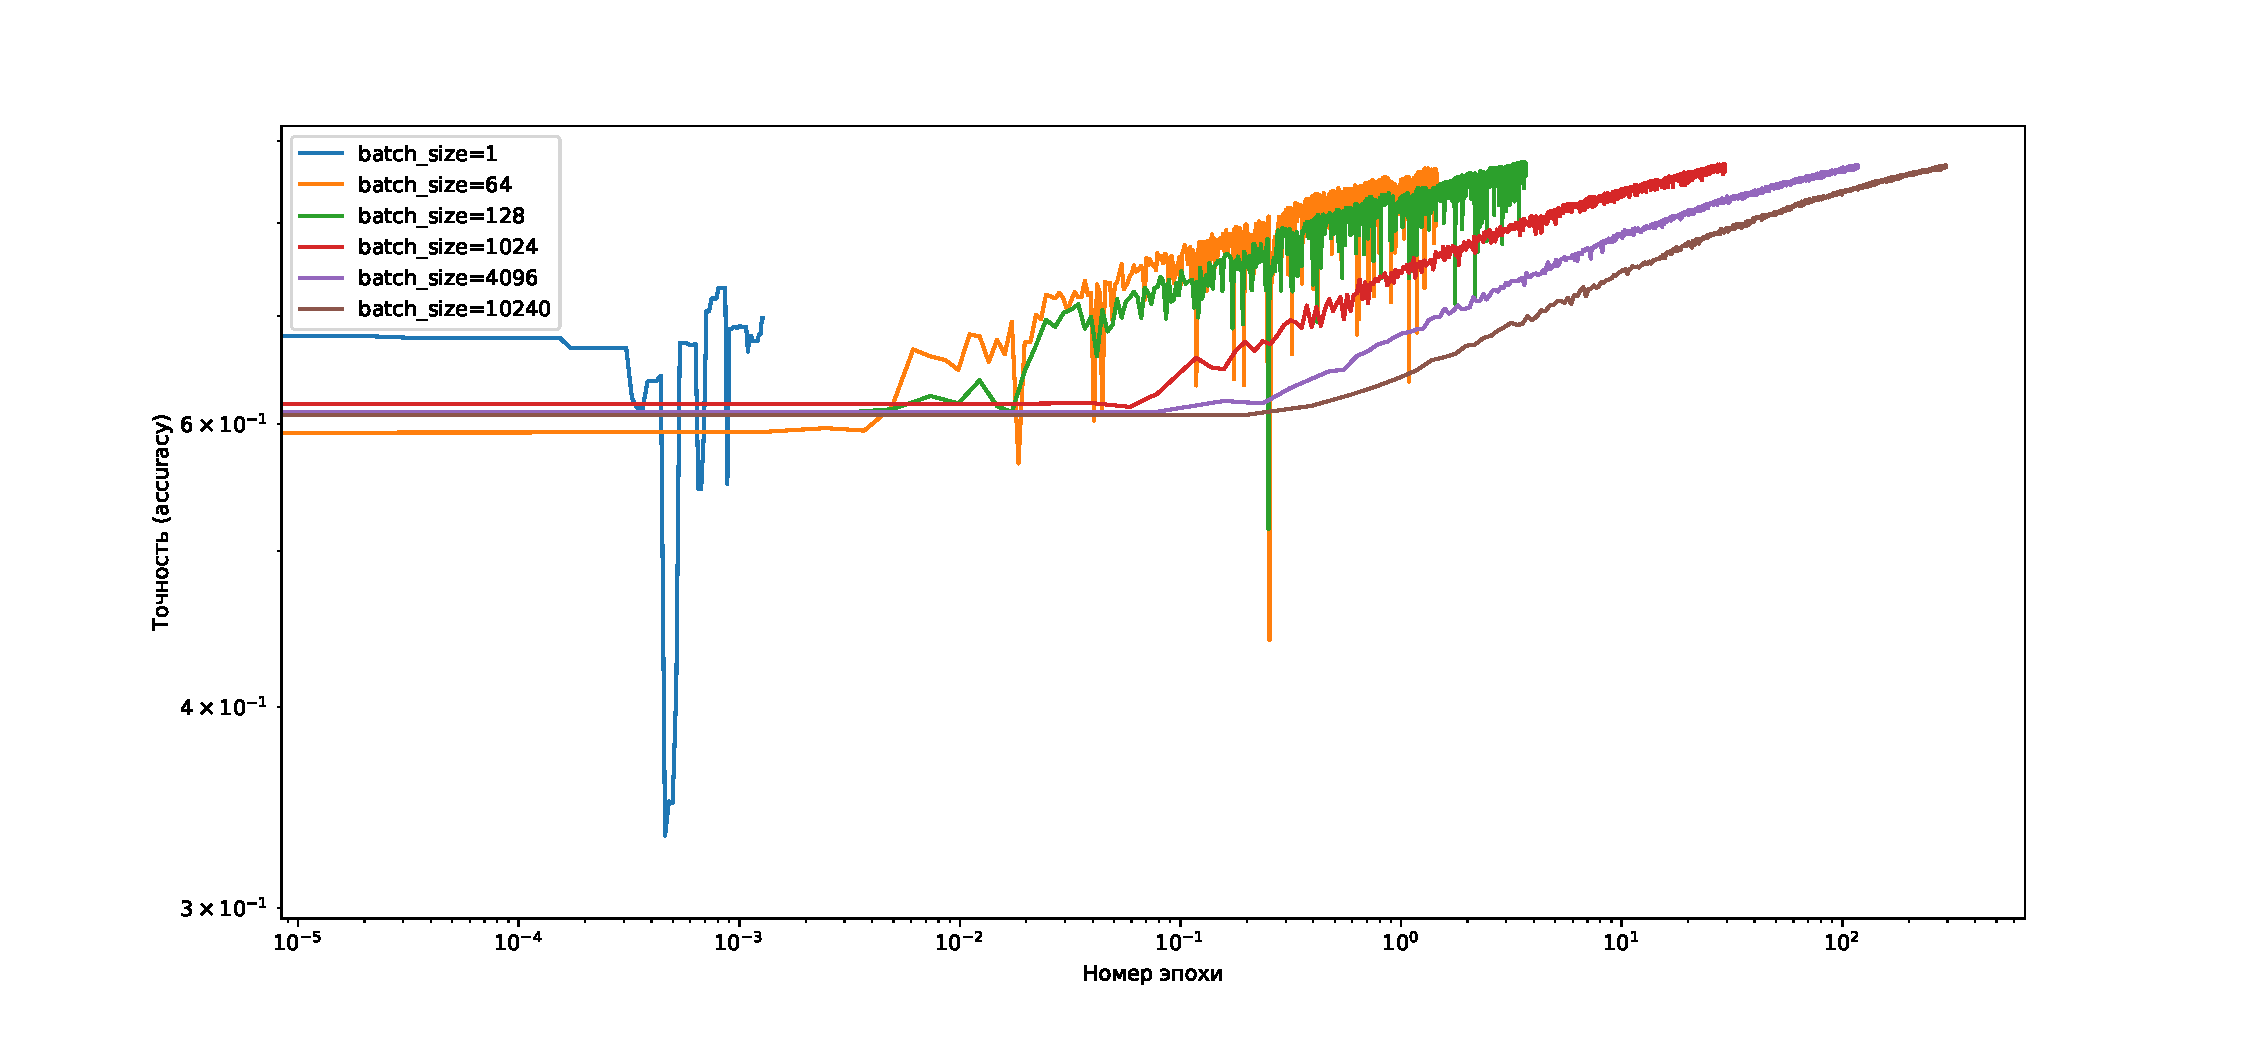
\includegraphics[width=0.5\textwidth, height=0.25\textheight]{../graphs/exp3_accuracy_SGD_bs_epoch_num_alpha=1_beta=0,01.pdf}
                    \end{center}
                \end{multicols}
            \end{figure}
        
            Можно заметить сильное увеличение дисперсии значений функции потерь с уменьшением размера подвыборки. Это объясняется тем, что при изменении весов на каждой итерации используется подвыборка для вычисления градиента, то есть приближенное значение, которое может сильно меняться от итерации к итерации, если размер подвыборки достаточно маленький.
            
            \subsubsection{Начальное приближение $w_0$}
            Начальное приближение нужно для инициализации весов модели. В данной работе были рассмотрены следующие варианты задания $w_0$:
            \begin{itemize}
                \item нулевой вектор
                \item вектор с координатами из $U(0, 1)$
                \item вектор с координатами из $U(100, 500)$
                \item вектор с координатами из $U(1000, 5000)$
                \item вектор с координатами из $U(10000, 50000)$
                \item вектор с координатами из $N(0, 1)$
                \item вектор с координатами из $N(0.5, 0.5)$
            \end{itemize}
            Графики зависимостей \ref{exp:dependencies_sgd} представлены на рис. \ref{exp4:sgd_func_time}, \ref{exp4:sgd_acc_time}, \ref{exp4:sgd_func_iter}, \ref{exp4:sgd_acc_iter}.
            \begin{figure}[H] \label{exp1}
                \begin{multicols}{2}
                    \begin{center}
                        \caption{Зависимость значения функции потерь от реального времени работы градиентного спуска} \label{exp4:sgd_func_time}
                        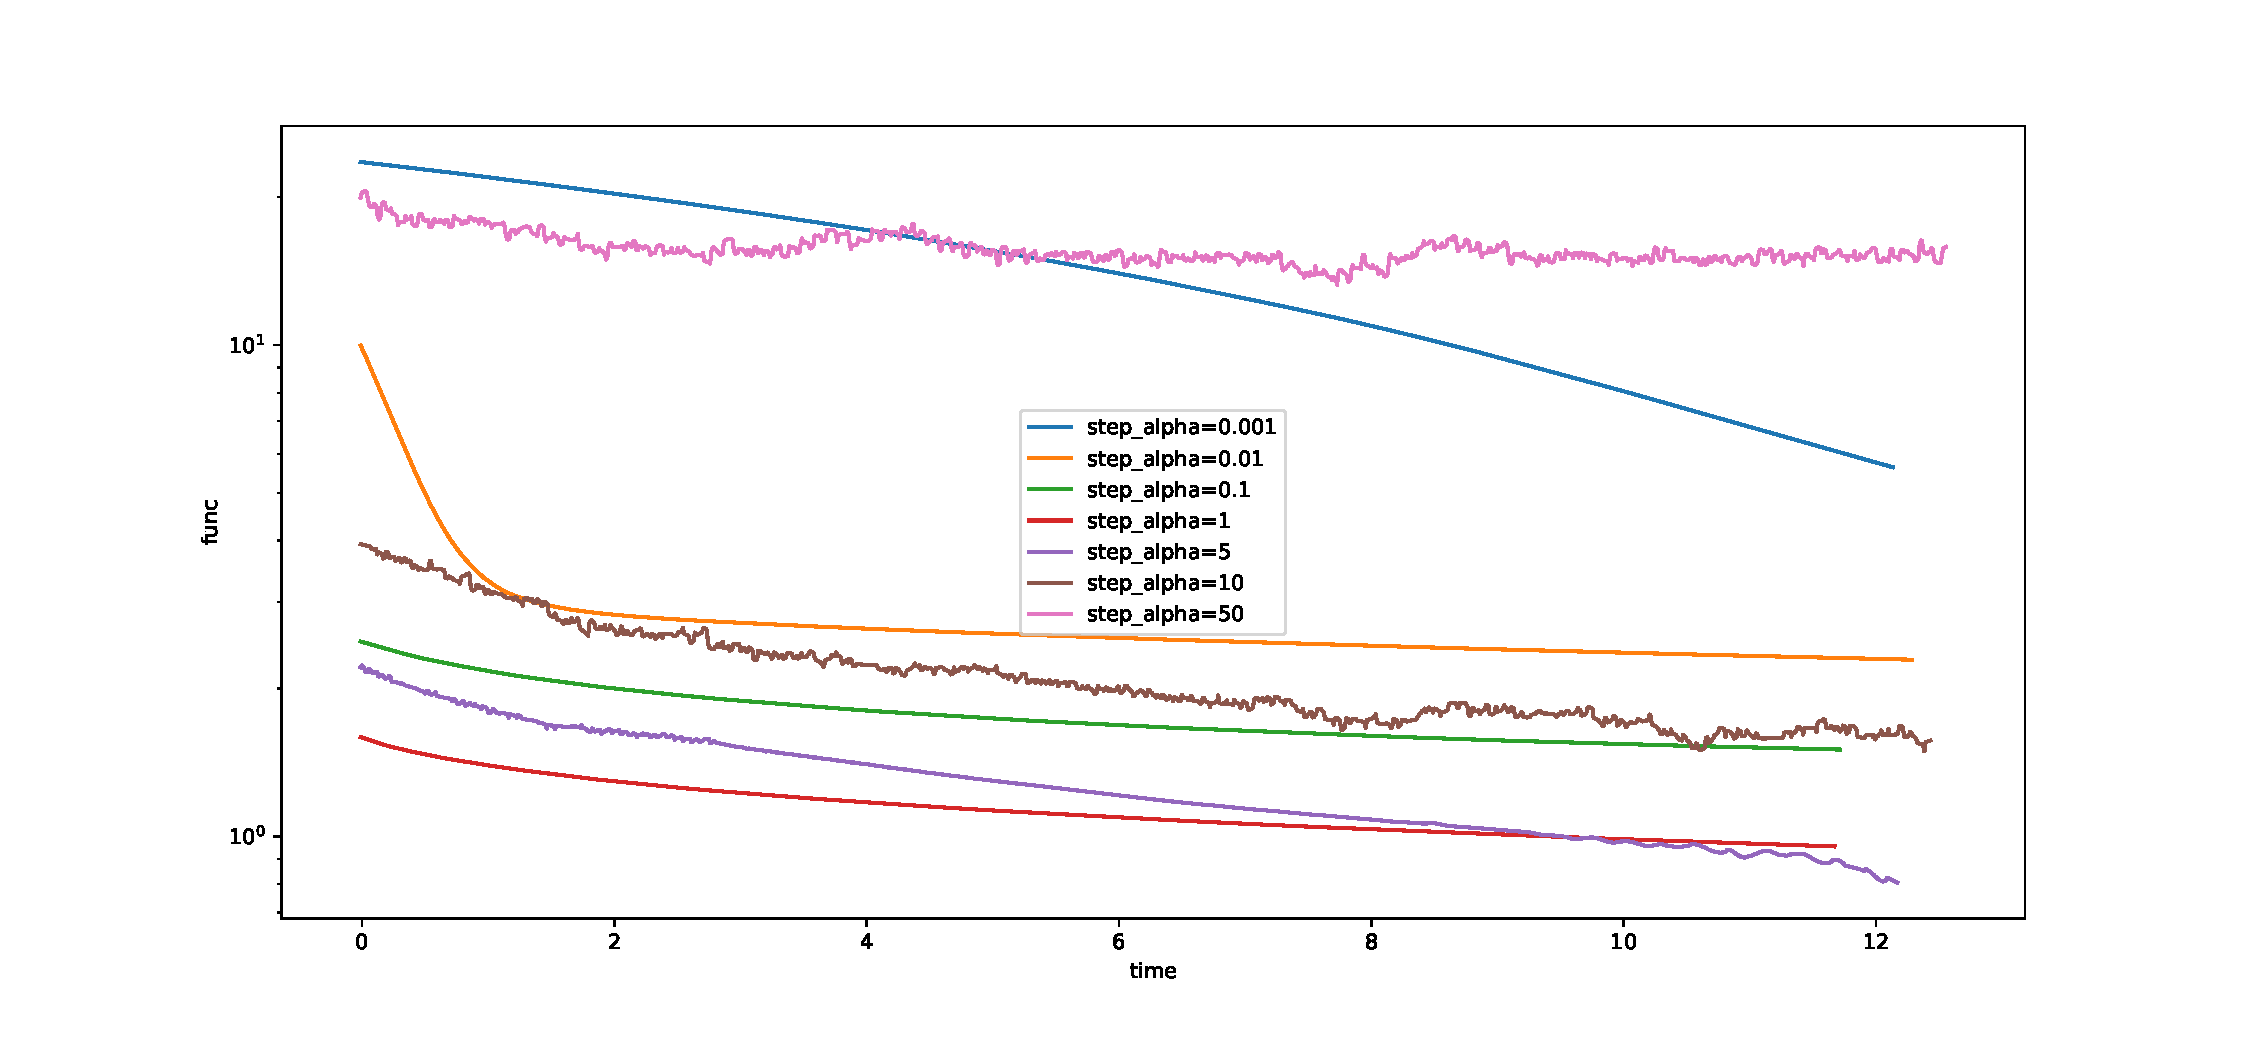
\includegraphics[width=0.5\textwidth, height=0.25\textheight]{../graphs/exp1_func_GD_alpha_time_beta=0,001.pdf}
                        
                        \caption{Зависимость значения точности (accuracy) от реального времени работы градиентного спуска} \label{exp4:sgd_acc_time}
                        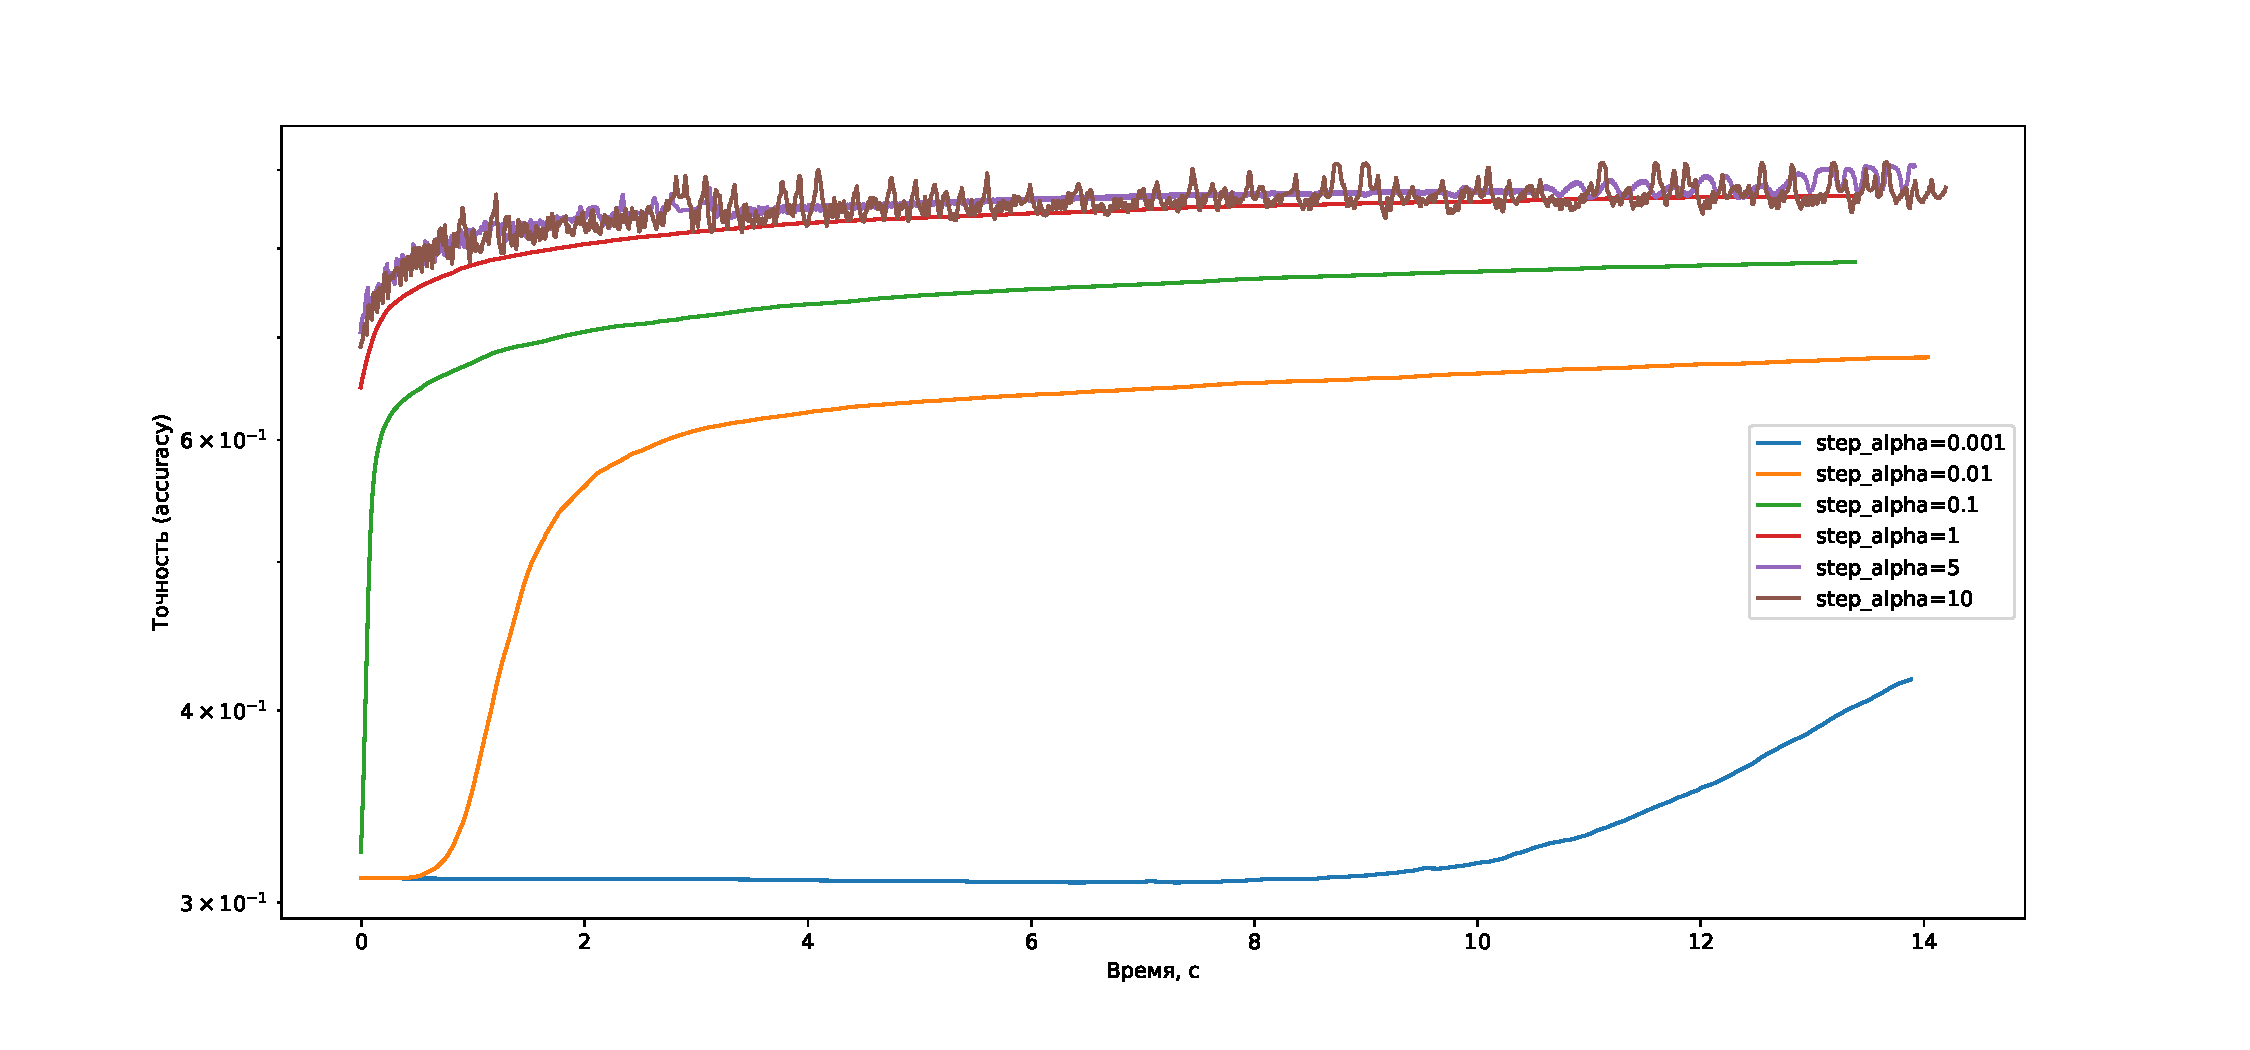
\includegraphics[width=0.5\textwidth, height=0.25\textheight]{../graphs/exp1_accuracy_GD_alpha_time_beta=0,001.pdf}
                        
                        \caption{Зависимость значения функции потерь от эпохи метода градиентного спуска} \label{exp4:sgd_func_iter}
                        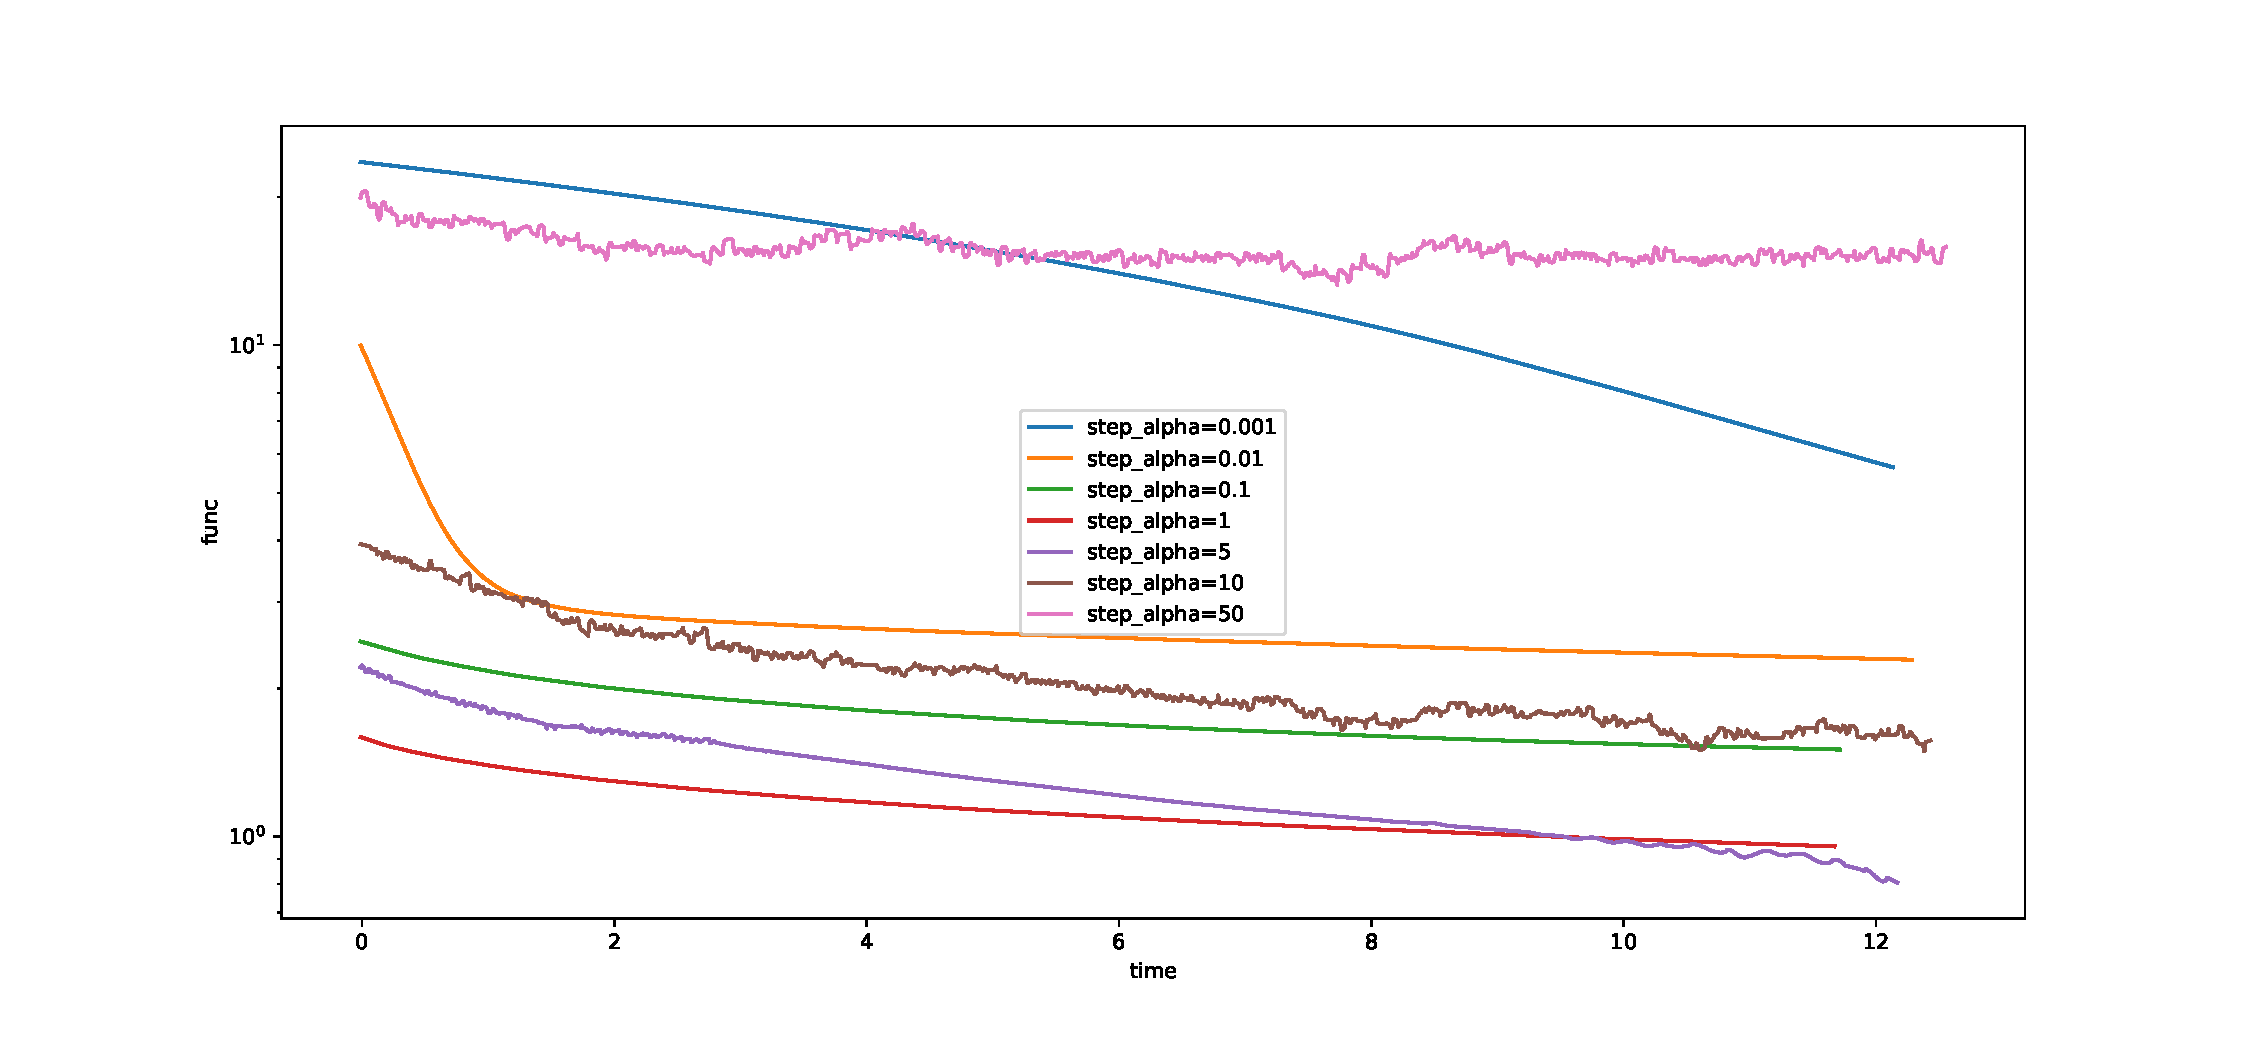
\includegraphics[width=0.5\textwidth, height=0.25\textheight]{../graphs/exp1_func_GD_alpha_time_beta=0,001.pdf}
                        
                        \caption{Зависимость значения точности (accuracy) от эпохи метода градиентного спуска} \label{exp4:sgd_acc_iter}
                        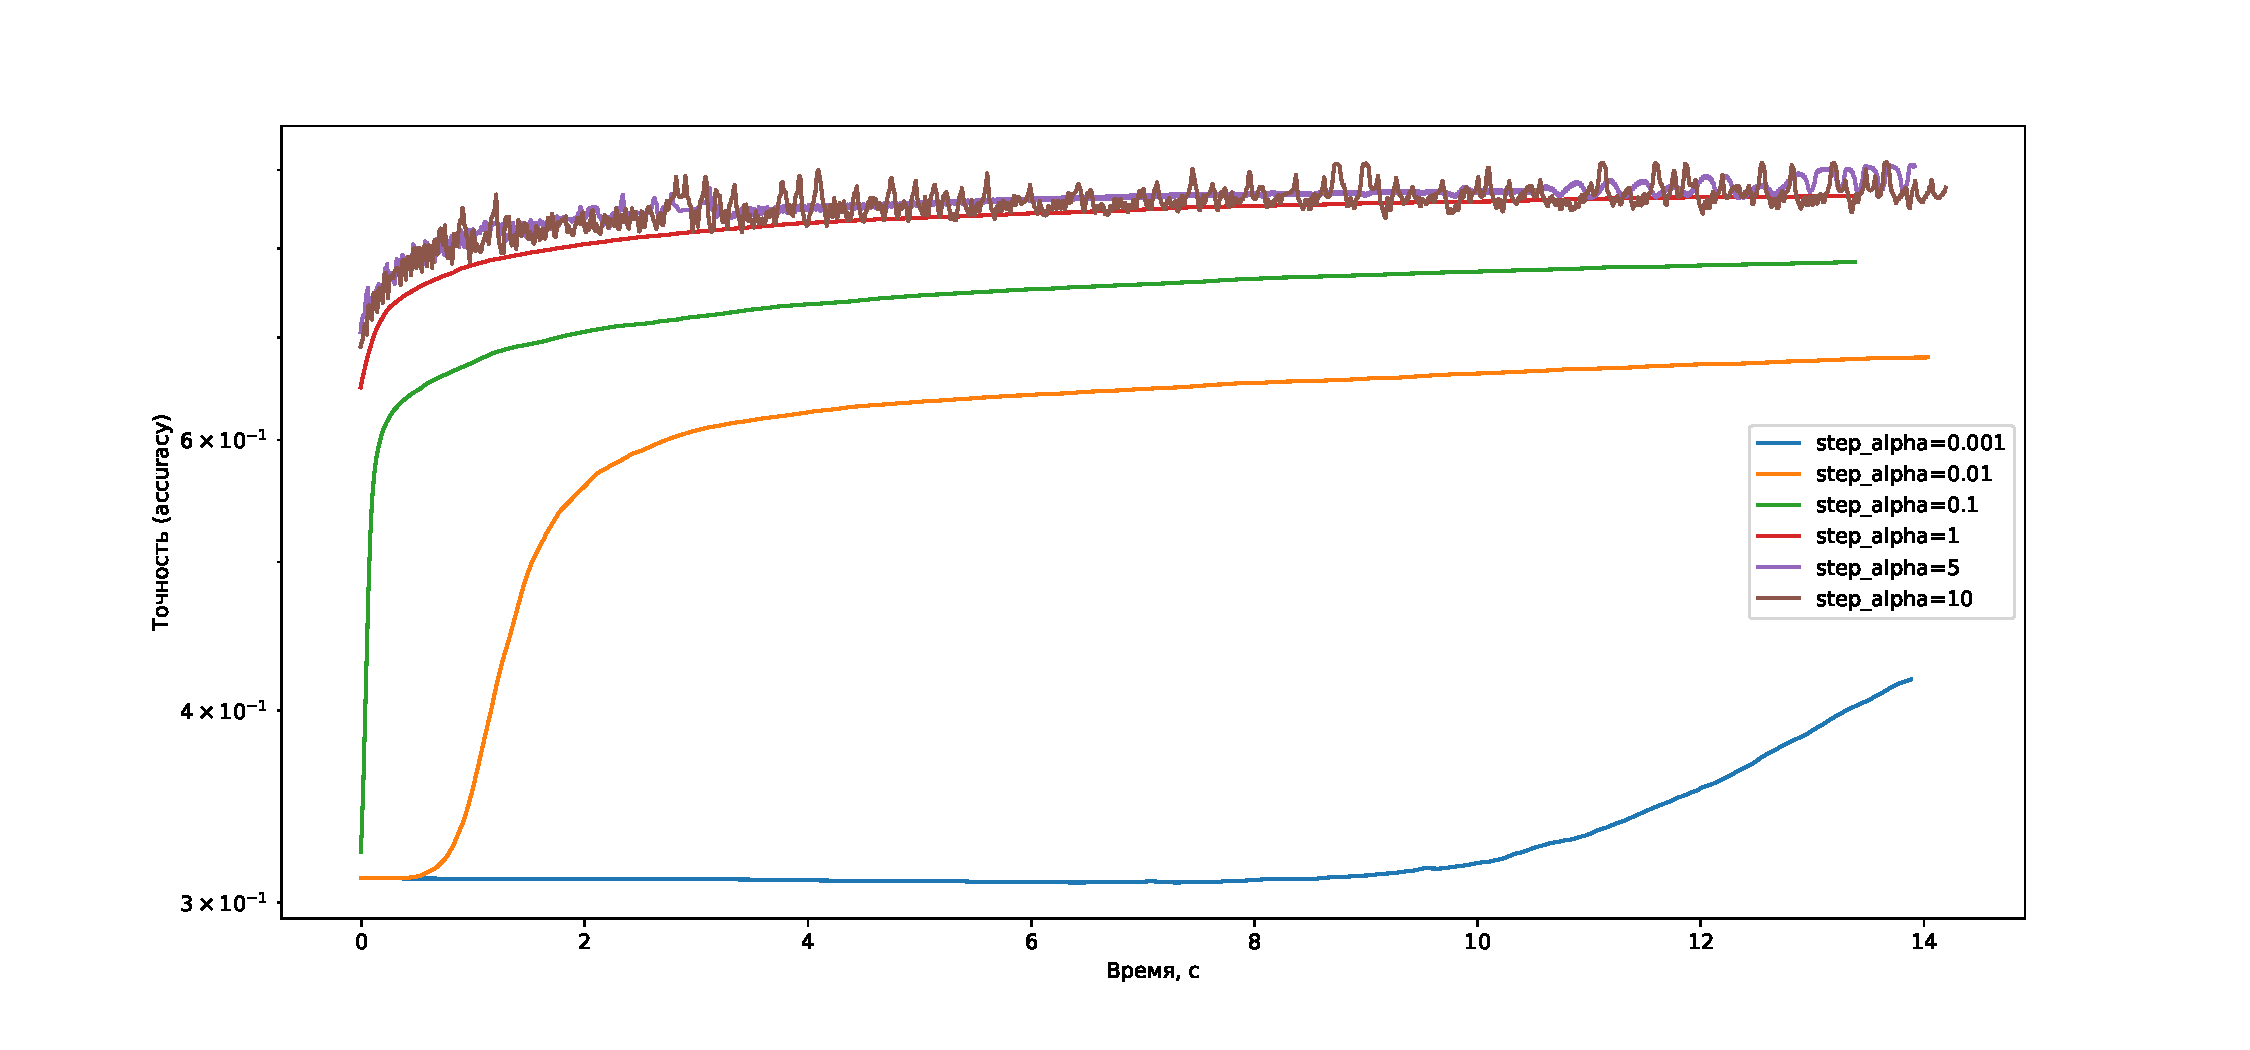
\includegraphics[width=0.5\textwidth, height=0.25\textheight]{../graphs/exp1_accuracy_GD_alpha_time_beta=0,001.pdf}
                    \end{center}
                \end{multicols}
            \end{figure}
        
            Из графиков видно, что лучшим вариантом инициализации весов оказался нулевой вектор.
            
        \subsection{Сравнение градиентного спуска и стохастического градиентного спуска}
            В данном разделе проведено сравнение методов по трем характеристикам:
            \begin{itemize}
                \item значения функции потерь
                \item точность (accuracy)
                \item время работы метода
            \end{itemize}
           Результаты экспериментов приведены на рис. \ref{sgd_gd_func_time}, \ref{sgd_gd_acc_time} и в таблице \ref{sgd_gd_time}
           \begin{figure}[H] \label{exp1}
               \begin{multicols}{2}
                   \begin{center}
                       \caption{Зависимость значения функции потерь от реального времени работы обычного и стохастического градиентного спуска} \label{sgd_gd_func_time}
                       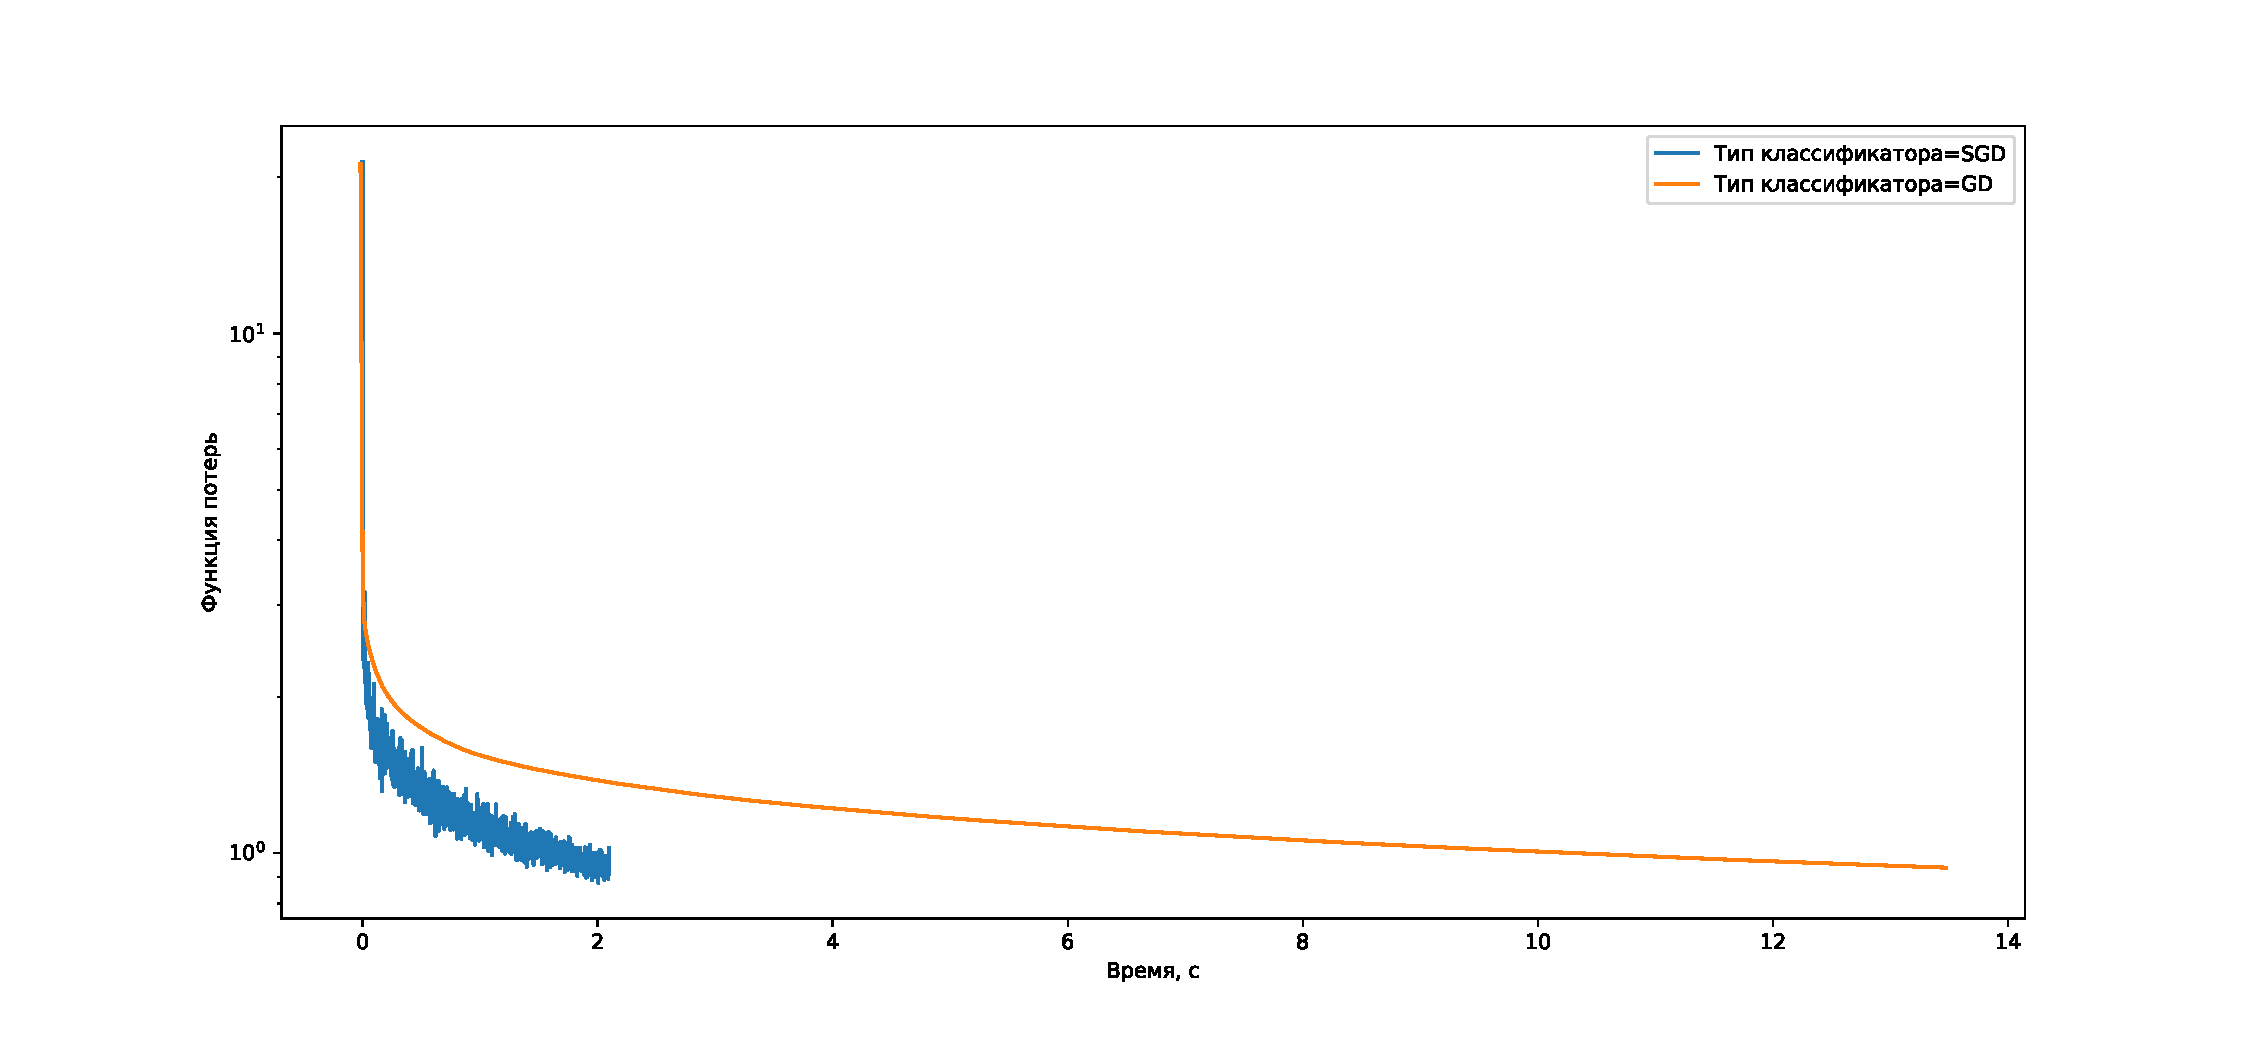
\includegraphics[width=0.5\textwidth, height=0.25\textheight]{../graphs/SGD_GD_func_alpha=1_beta=0,001_bs=1024.pdf}
                       
                       \caption{Зависимость значения точности (accuracy) от реального времени работы обычного и стохастического градиентного спуска} \label{sgd_gd_acc_time}
                       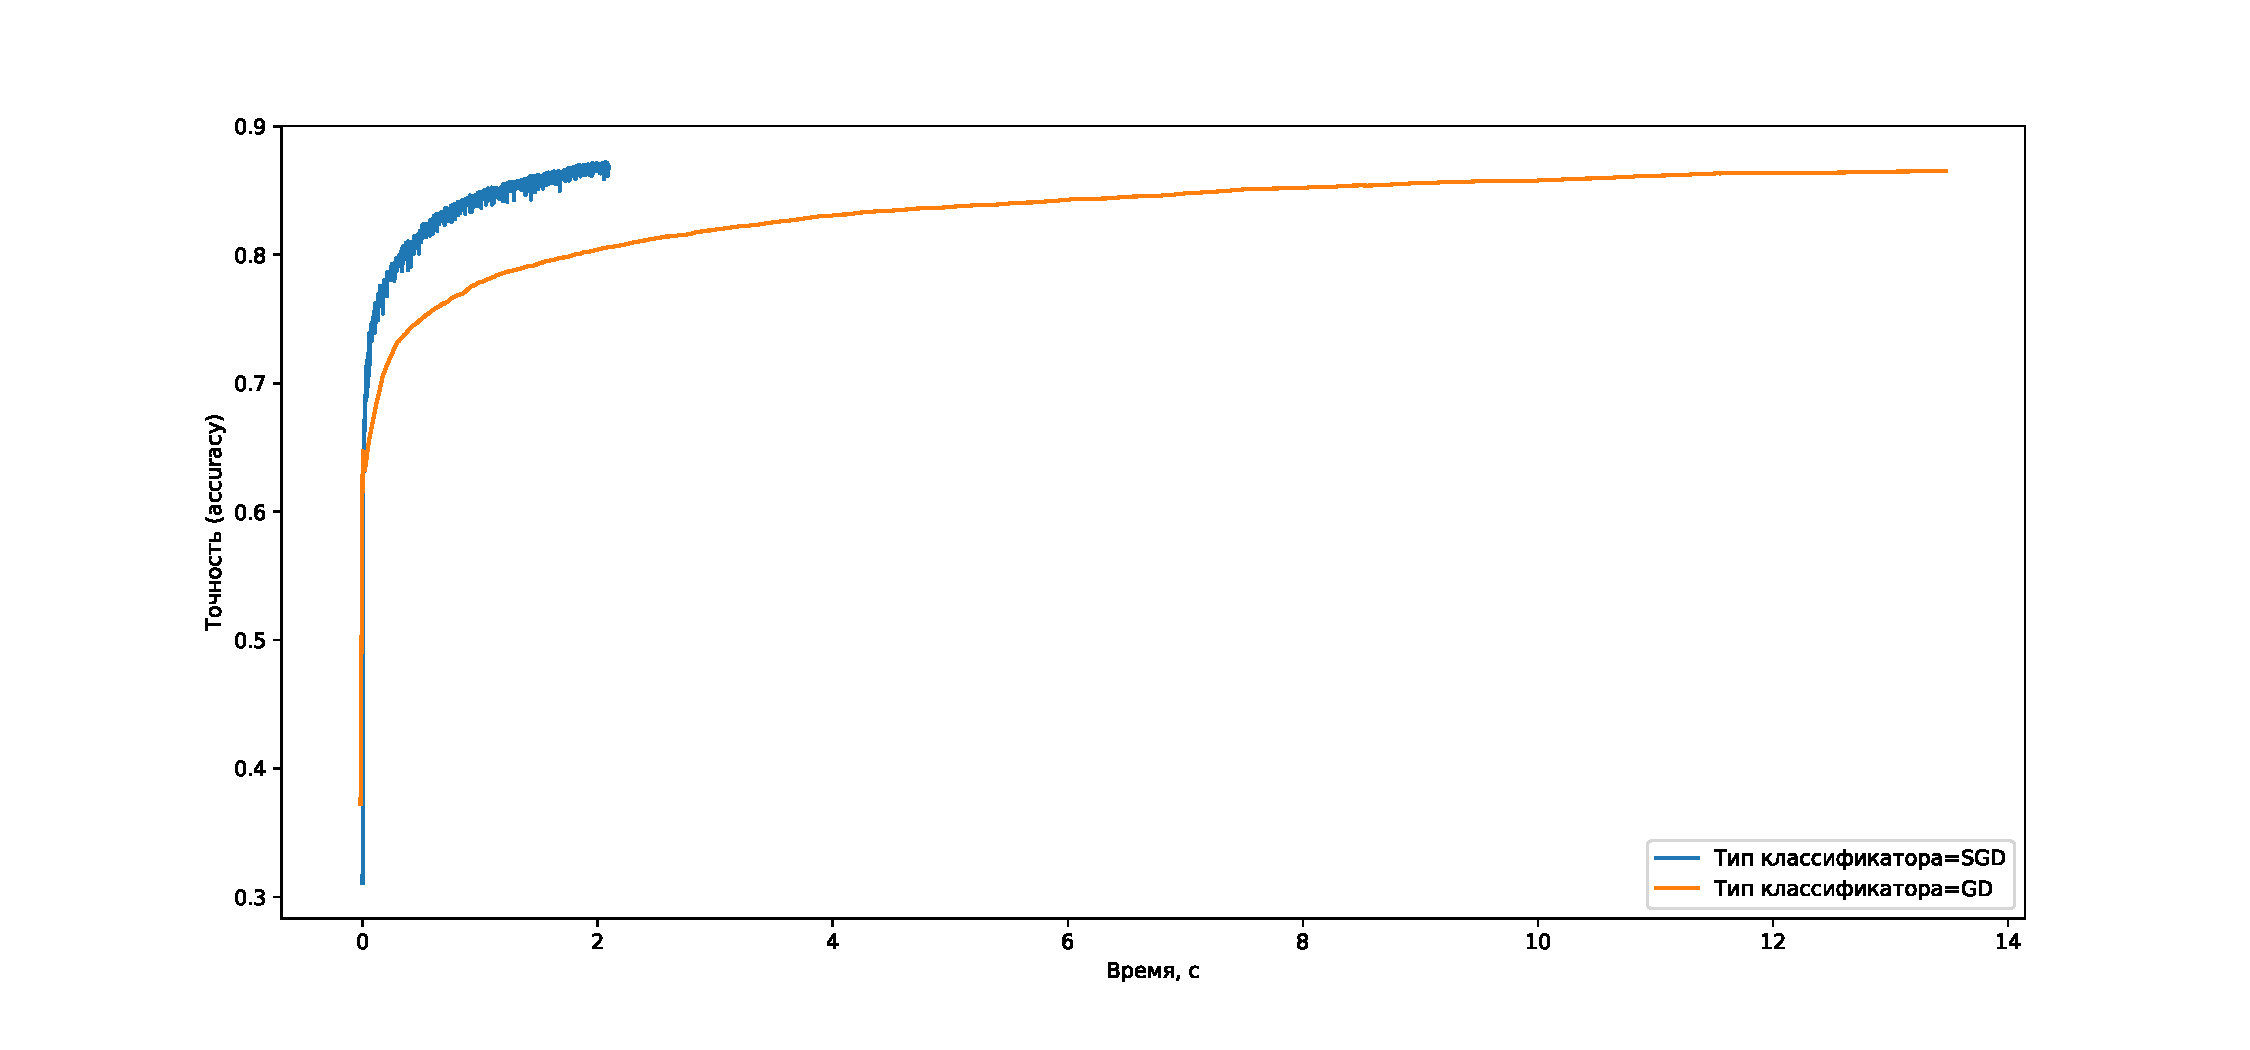
\includegraphics[width=0.5\textwidth, height=0.25\textheight]{../graphs/SGD_GD_accuracy_alpha=1_beta=0,001_bs=1024.pdf}
                   \end{center}
               \end{multicols}
           \end{figure}
       
           \begin{table}[H]
               \caption{Среднее время работы методов оптимизации}
               \label{sgd_gd_time}
               \begin{center}
                   \begin{tabular}{|c|c|}  
                       \hline 
                       Метод & Среднее время работы, с \\ 
                       \hline 
                       Градиентный спуск & 8.852 \\ 
                       \hline 
                       Стохастический градиентный спуск & 1.964 \\ 
                       \hline 
                   \end{tabular}
               \end{center}
           \end{table}
       
           Из приведенных выше графиков видно, что стохастический градиентный спуск сходится быстрее, причем к более хорошему оптимуму, чем обычный градиентный спуск, но сходимость с б$\acute{o}$льшей дисперсией значений функции потерь. Таблица \ref{sgd_gd_time} показывает, что стохастический градиентный спуск работает в несколько раз быстрее.
            
        \subsection{Лемматизация и удаление стоп-слов}
            В этом эксперименте проводится лемматизация, в которой считается, что все слова в тексте - глаголы. Удаляются все стоп-слова. В таблице \ref{simple_lemma_stopword_dimension} приведено сравнение метода градиентого спуска до преобразования текста и после. Все измерения проведены для градиентного спуска с параметрами: $step\_alpha=1$, $step\_beta=0.001$.
            
            \begin{table}[H]
                \begin{center}
                \caption[Caption1]{Влияние предобработки на качество алгоритма}
                \label{simple_lemma_stopword_dimension}
                    \begin{tabular}{|c|c|c|c|}  
                        \hline 
                        Метод предобработки & Точность & Среднее время работы, с & Количество признаков \\ 
                        \hline 
                        (1), (2) & 0.8800 & 13.59 & 91840 \\ 
                        \hline 
                        (1), (2), (3), (4) & 0.8766 & 13.21 & 83530 \\
                        \hline 
                        (1), (2), (3) & \textbf{0.9016} & \textbf{13.09} & 83400 \\ 
                        \hline 
                    \end{tabular}
                
                \begin{enumerate}
                    \item[(1)] - приведение к нижнему регистру
                    \item[(2)] - удаление всех символов, отличных от букв и цифр
                    \item[(3)] - лемматизация
                    \item[(4)] - удаление стоп-слов
                \end{enumerate}
                \end{center}
            
            \end{table}
        Как видно из таблицы - с уменьшением признакового пространства уменьшается и время работы алгоритма. Можно заметить интересную особенность: удаление стоп-слов понижает точность классификации. Есть предположение, что удаление стоп-слов - не самая лучшая идея в данной задаче, так как в них есть такие, как <<aren't>>, <<didn't>>, которые указывают на отрицание. Пример: you aren't nice -> you nice (после удаления стоп-слов).
        
        \subsection{Сравнение представлений BagOfWords и TF-IDF с различными значениями параметра min\_df}
            В данном разделе рассматривается зависимость качества, времени работы алгоритма и размер признакового пространства от:
            \begin{itemize}
                \item использовалось представление BagOfWords или TF-IDF
                \item параметров min\_df и max\_df конструкторов
            \end{itemize}
            Не ограничивая общности рассмотрим различные значения только для \textbf{min\_df}, так как $\textbf{max\_df} = 1 - \textbf{min\_df}$ дает эквивалентное преобразование, при условии $max\_df \in [0, 1], min\_df \in [0, 1]$
            Графики зависимостей представлены на рис. \ref{exp5:gd_bow_tfidf_accuracy}, \ref{exp5:min_df_accuracy}, \ref{exp5:gd_bow_size_time}
            \begin{figure}[H] \label{exp5}
                \begin{multicols}{2}
                    \begin{center}
                        \caption{Зависимость  точности от типа представления} \label{exp5:gd_bow_tfidf_accuracy}
                        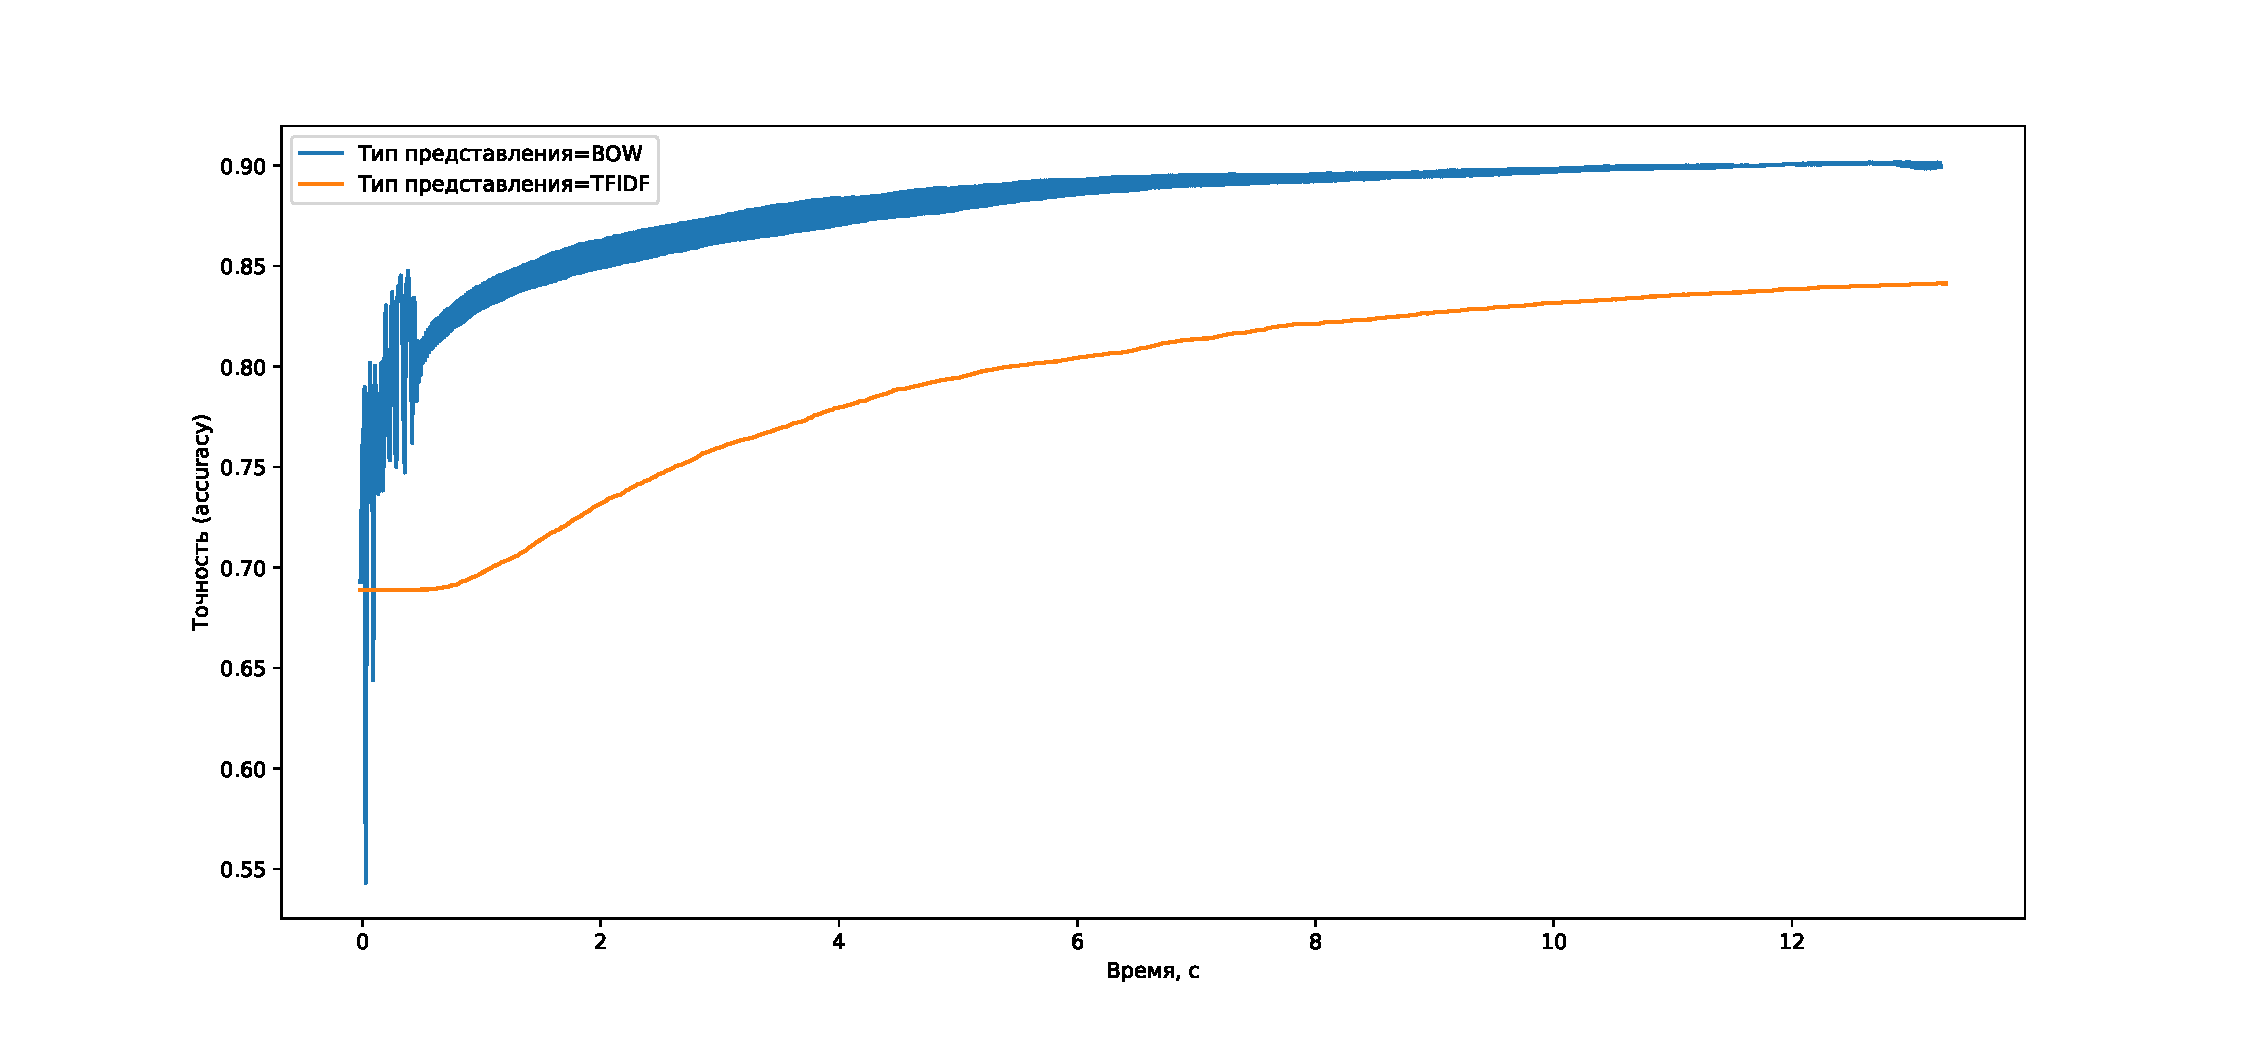
\includegraphics[width=0.5\textwidth, height=0.25\textheight]{../graphs/GD_BOW_TFIDF_alpha=1_beta=0,001_train_size=83530.pdf}
                        
                        \caption{Зависимость  точности от параметра конструктора min\_df} \label{exp5:min_df_accuracy}
                        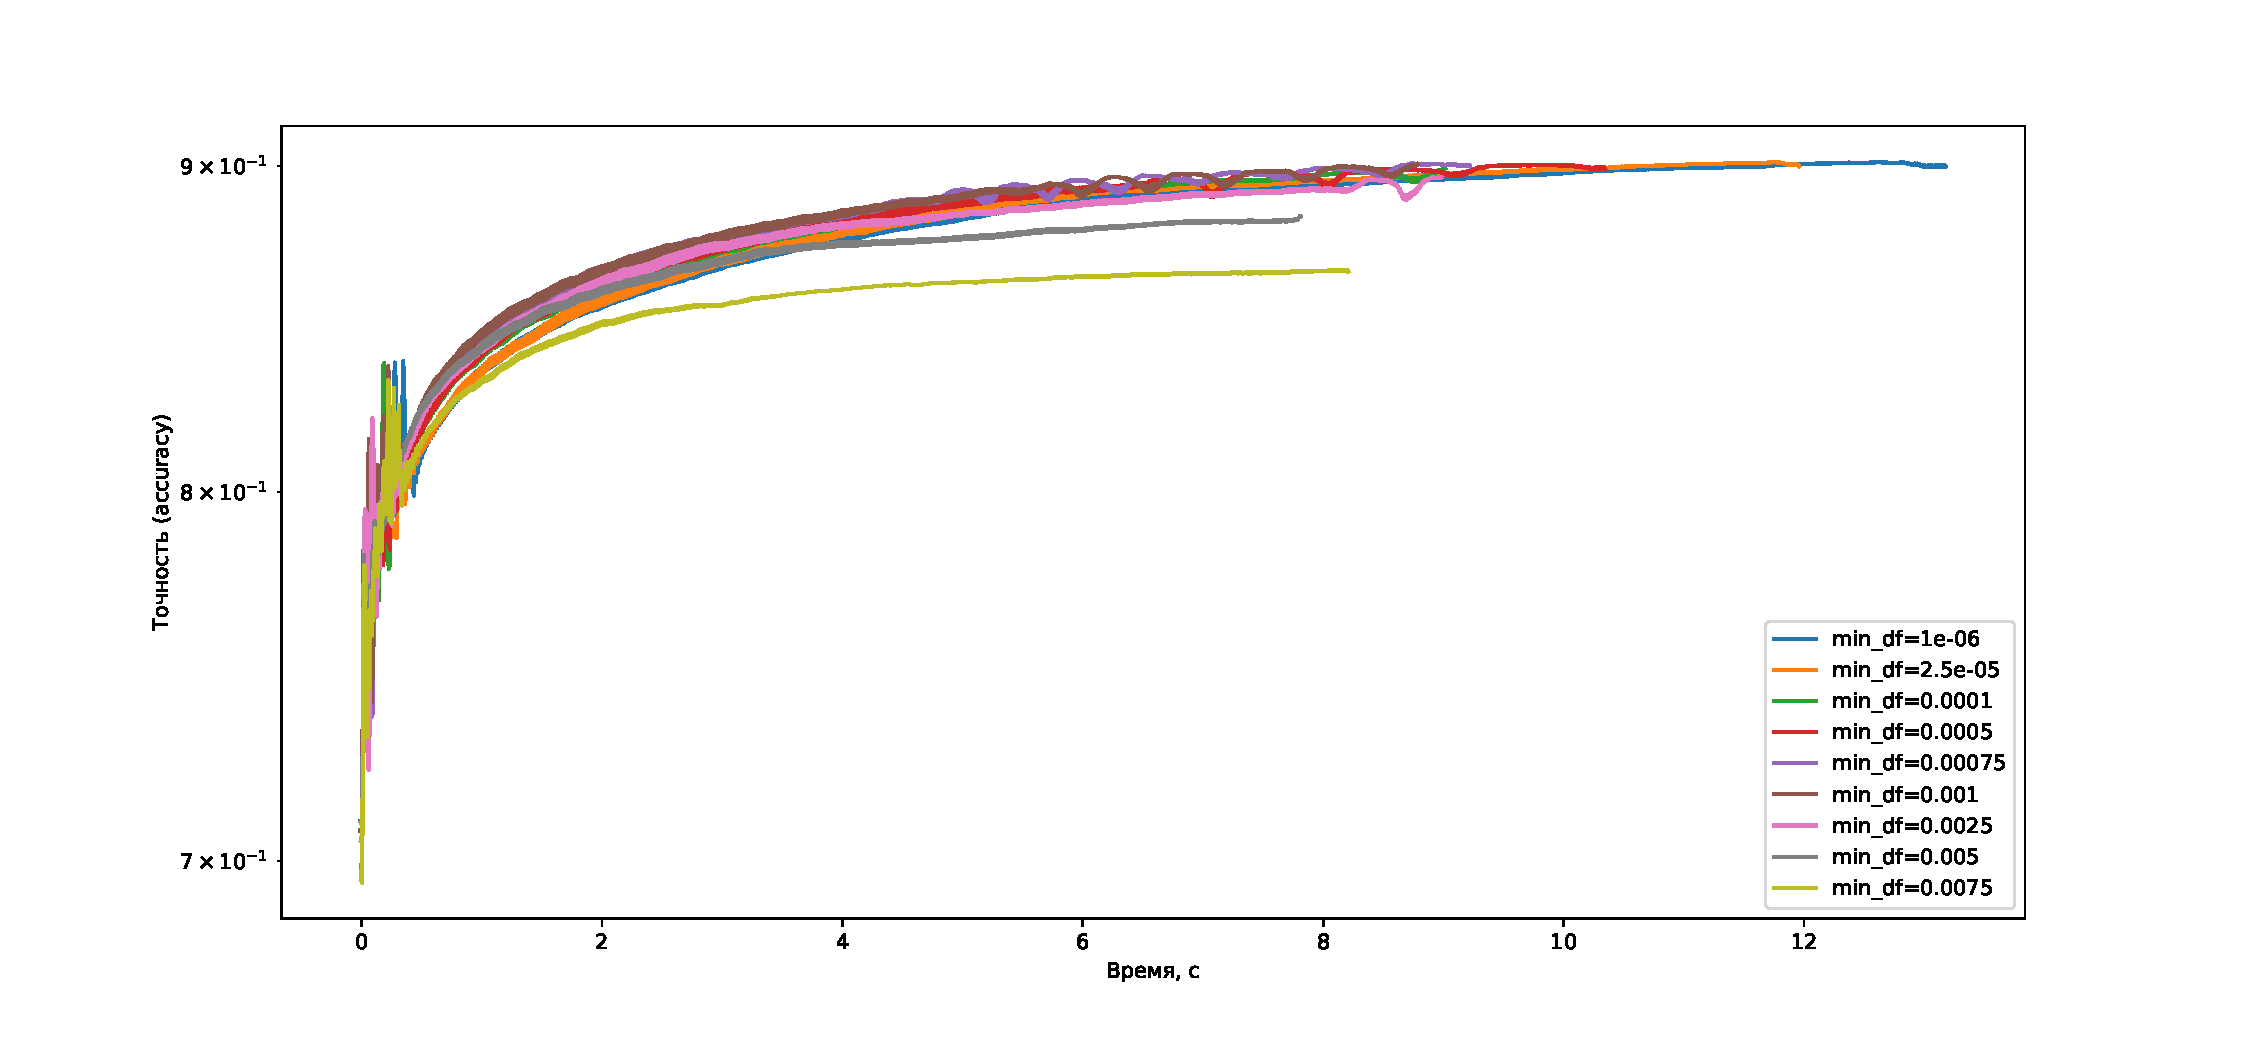
\includegraphics[width=0.5\textwidth, height=0.25\textheight]{../graphs/GD_min_df_accuracy.pdf}
                    \end{center}
                \end{multicols}
            \end{figure}
        
            \begin{figure}[H] \label{exp5}
                    \begin{center}
                        \caption{Зависимость размера признакового пространства от параметра конструктора min\_df} \label{exp5:gd_bow_size_time}
                        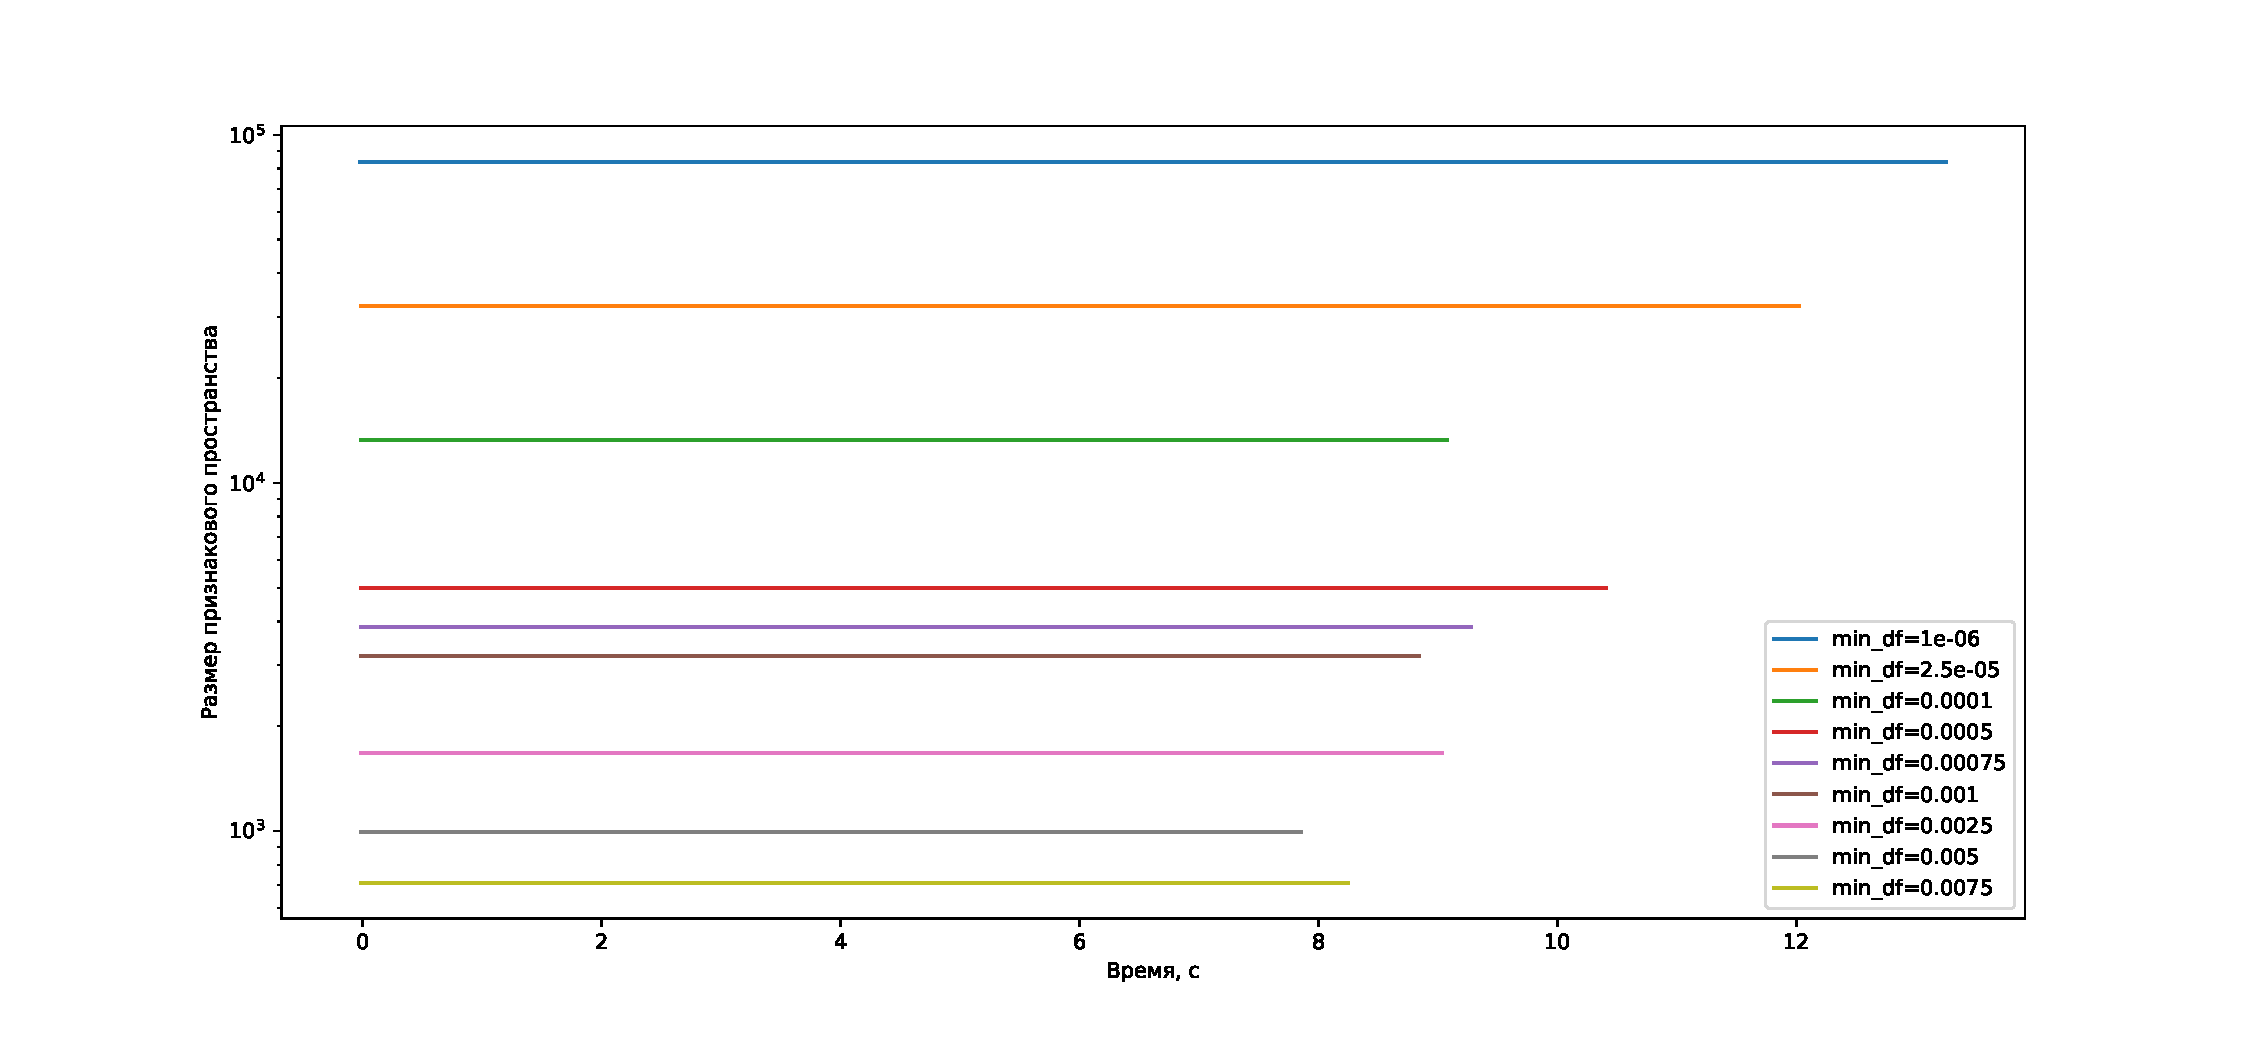
\includegraphics[width=0.5\textwidth, height=0.25\textheight]{../graphs/GD_BOW_min_df_train_size.pdf}
                    \end{center}
            \end{figure}
            Из рис. \ref{exp5:gd_bow_tfidf_accuracy} видно, что:
            \begin{itemize}
                \item при использовании представления BagOfWords достигается наибольшее значение точности (это может быть связано с тем, что токсичные комментарии более заспамленные, поэтому TF-IDF занижает вклад <<спам-слов>> в таких сообщениях)
                \item время работы метода не зависит от использования представлений BagOfWords или TF-IDF (является следствием следующего пункта)
                \item размерность признакового пространства не зависит от типа представления (так как в BagOfWords и TF-IDF различаются только значения признаков, но не их количество)
            \end{itemize}
            
            Из рис. \ref{exp5:min_df_accuracy} видно, что:
                \begin{itemize}
                    \item при достаточно маленьких значениях \textbf{min\_df} (до 0.0025) достигается практически одинаковая точность, но если брать значения больше 0.0025, то точность классификации ухудшается.
                \end{itemize}   
                         
            Из рис. \ref{exp5:gd_bow_size_time} можно заметить, что:
            \begin{itemize}
                 \item с увеличением значения \textbf{min\_df} уменьшается время работы алгоритма (следствие из пункта ниже)
                 \item с увеличением значения \textbf{min\_df} уменьшается размерность признакового пространства
            \end{itemize}   
        
    \section{Применение лучшего алгоритма к тестовой выборке и анализ ошибок, допущенных алгоритмом}
        Применим к тестовой выборке лучший алгоритм\footnote{SGD, $step\_alpha = 1$, $step\_beta = 0.001$, $batch\_size = 1024$ с преобразованием BOW, лемматизацией, но без удаления стоп-слов.}
        Получено значение точности: \textbf{0.8854}
        
        Проанализируем ошибки алгоритма:
        \begin{itemize}
            \item <<i \textbf{didn t} screw up  i lapsed  when you revert  you should examine what the previous editor did  as several reverters are doing  reverting again me at amin al husseini so blindly they do \textbf{not} notice they are removing intermediate edits involving correction of dates and spellings  it means that this is personal  or ideological  and \textbf{not} motivated by intelligent assessments of the merits>>.
            
            Данный комментарий был классифицирован, как токсичный. Есть предположение, что алгоритм ошибается в тех комментариях, где есть много отрицаний (чаще такие комменатарии имеют негативный оттенок).
        \end{itemize}
    
    \section{Бонусная часть}
        \subsection{Исследование параметра \textbf{ngramm\_range} у TfidfTransformer}
            Данный параметр отвечает за количество $n$-грамм, которые будут добавлены в признаковое пространство. $n$-грамма - некоторая последовательность из $n$ элементов (в данном случае элементы - слова). 
            
            Результаты экспериментов представлены на графике ниже (рис. \ref{extra1:ngramm_accuracy})
            \begin{figure}[H] \label{extra1}
                    \begin{center}
                        \caption{Зависимость  точности значения параметра \textbf{ngramm\_range}} \label{extra1:ngramm_accuracy}
                        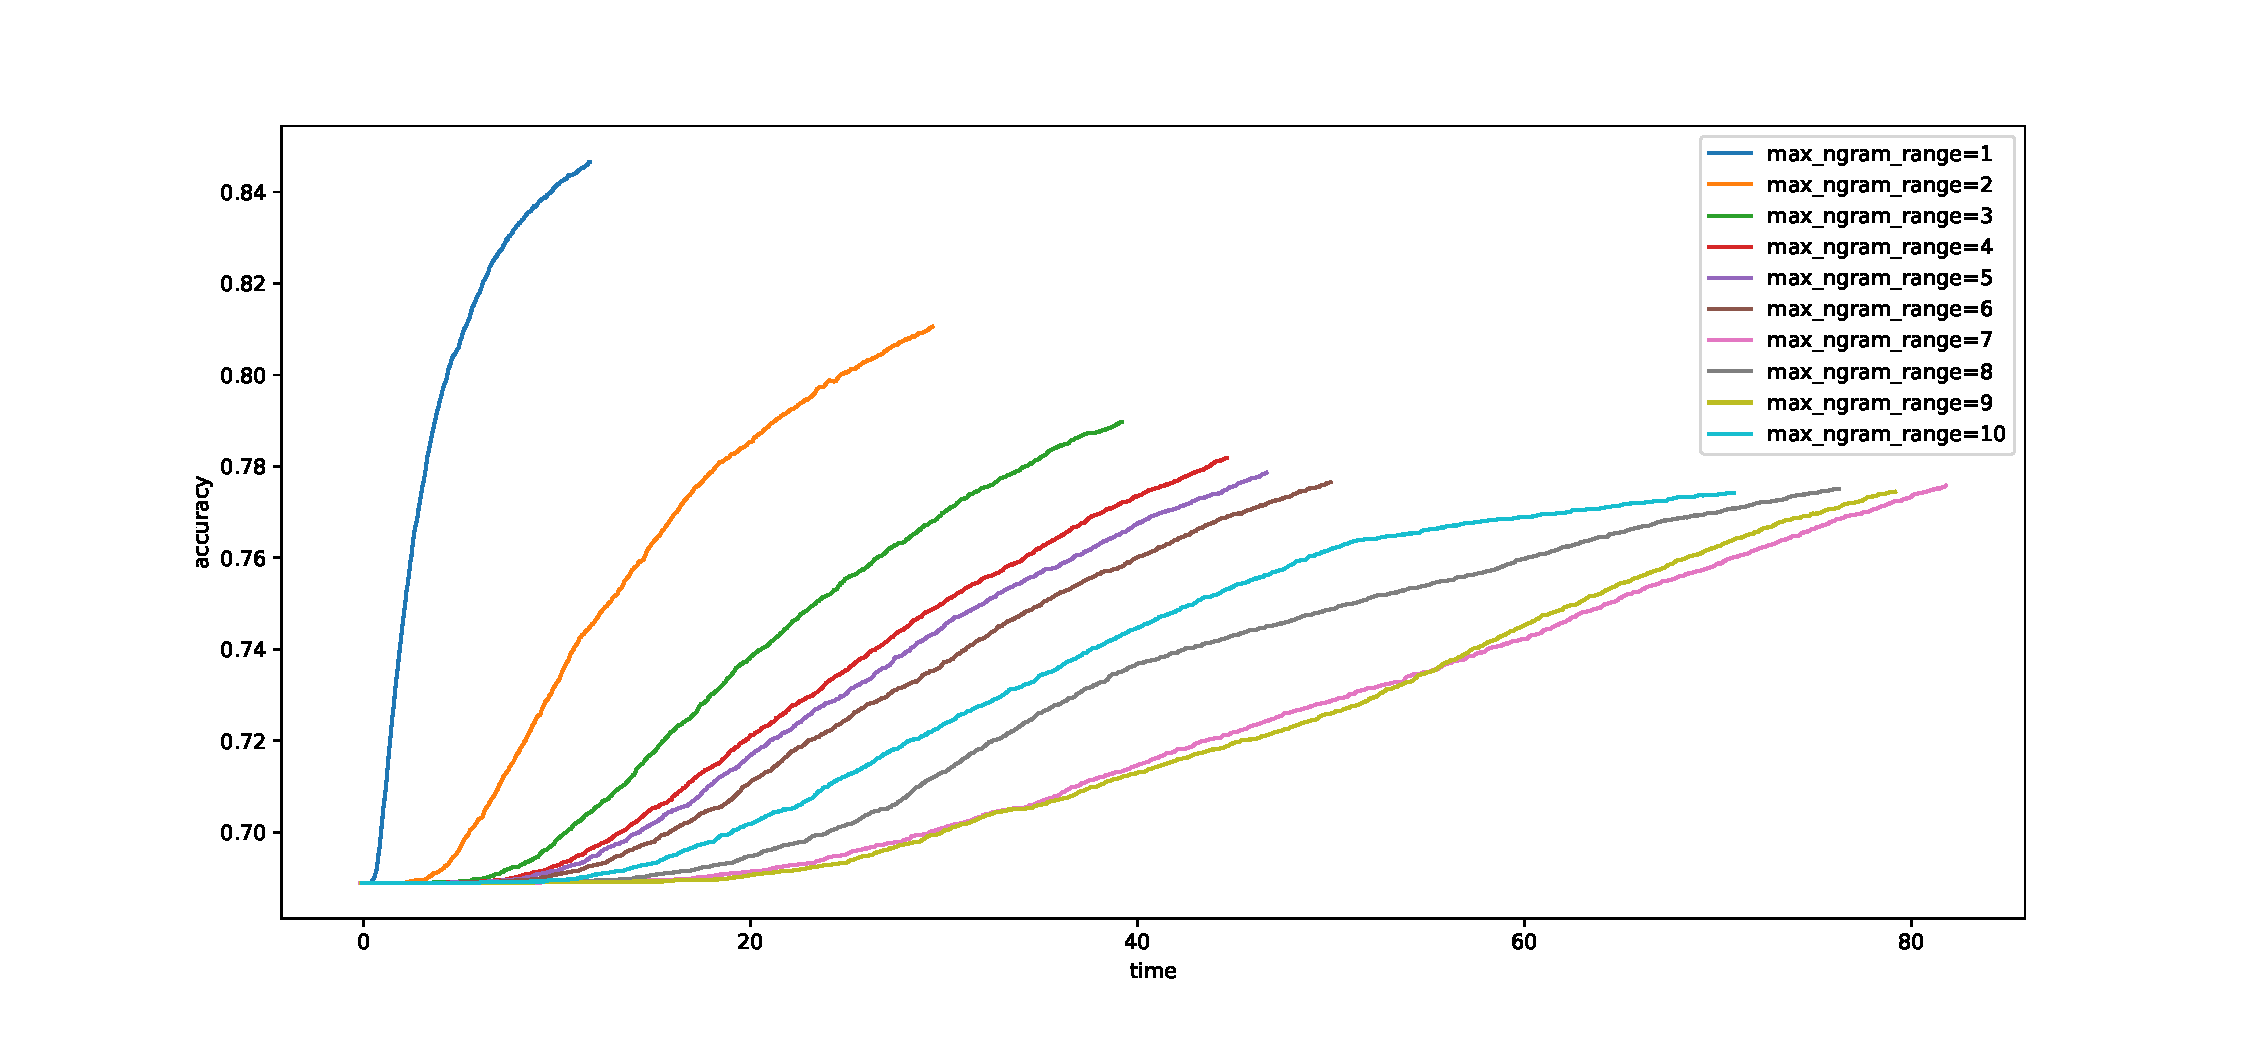
\includegraphics[width=0.8\textwidth, height=0.25\textheight]{../graphs/ngram_exp.pdf}
                    \end{center}
            \end{figure}
            Можно заметить, что с увеличением значения параметра \textbf{ngramm\_range} увеличивается и время работы алгоритма.
            
    
       
        
        
            
\end{document}